%\documentclass[ignorenonframetext, professionalfonts, hyperref={pdftex, unicode}]{beamer}
\documentclass[pdftex,12pt,a4paper]{report}
\usepackage{beamerarticle}

\usetheme{Copenhagen}
\usecolortheme{wolverine}

%Packages to be included
\usepackage{graphicx}

\usepackage[T2A,T1]{fontenc}
\usepackage[utf8]{inputenc}
\usepackage[russian]{babel}

%%\usepackage[orientation=landscape, size=custom, width=16, height=9.75, scale=0.5]{beamerposter}

\usepackage{textcomp}

%\usepackage{beamerthemesplit}

\usepackage{ulem}

\usepackage{verbatim}

\usepackage{ucs}

\usepackage{url}

\usepackage{listings}
\lstloadlanguages{bash}

\lstset{escapechar=`,
	extendedchars=false,
	language=sh,
	frame=single,
	tabsize=2, 
	columns=fullflexible, 
%	basicstyle=\scriptsize,
	keywordstyle=\color{blue}, 
	commentstyle=\itshape\color{brown},
%	identifierstyle=\ttfamily, 
	stringstyle=\mdseries\color{green}, 
	showstringspaces=false, 
	numbers=left, 
	numberstyle=\tiny, 
	breaklines=true, 
	inputencoding=utf8,
	keepspaces=true,
	morekeywords={u\_short, u\_char, u\_long, in\_addr}
	}

\definecolor{darkgreen}{cmyk}{0.7, 0, 1, 0.5}

\lstdefinelanguage{diff}
{
    morekeywords={+, -},
    sensitive=false,
    morecomment=[l]{//},
    morecomment=[s]{/*}{*/},
    morecomment=[l][\color{darkgreen}]{+},
    morecomment=[l][\color{red}]{-},
    morestring=[b]",
}

\author[Epam]{{\bf Epam}\\Low Level Programming Department}

%\institution[EPAM]{EPAM}
\logo{\includegraphics[width=1cm]{logo.png}}

\usepackage[unicode=true]{hyperref}
\hypersetup{
    pdfkeywords={Linux},
    bookmarksnumbered=true,
    bookmarksopen=true,
    bookmarksopenlevel=1,
    colorlinks=true,
    pdfstartview=Fit,
    pdfpagemode=UseOutlines,
    pdfpagelayout=TwoPageRight
}

\title{Software development in Linux environment\\Handbook}

\mode<all>{
\usepackage{pgf,tikz}
% built files
\definecolor{bfile}{rgb}{.9,0.9,0.9}
% distributed generated files
\colorlet{dgfile}{yellow}
% auto* input file
\colorlet{afile}{green!33}
% tools
\definecolor{tfile}{rgb}{1.0,0.5,0.5}

\tikzstyle{afile}=[draw,fill=afile,shape=rectangle,inner sep=1ex]
\tikzstyle{bfile}=[draw,fill=bfile,shape=rectangle,inner sep=1ex]
\tikzstyle{dgfile}=[draw,fill=dgfile,shape=rectangle,inner sep=1ex]
\tikzstyle{tfile}=[draw,fill=tfile,shape=rectangle,inner sep=1ex]

\newcommand\arr[1][]{\draw[thick,->,#1]}
\def\afile{\node[style=afile]}
\def\bfile{\node[style=bfile]}
\def\dgfile{\node[style=dgfile]}
\def\tfile{\node[style=tfile]}

\newcommand{\filename}[1]{{\color{blue}{\textit{\begingroup \urlstyle{sf}\Url{#1}}}}}
\newcommand{\filenamew}[1]{{{\textit{\begingroup \urlstyle{sf}\Url{#1}}}}}
\newcommand{\command}[1]{\texttt{#1}}

}

\begin{document}

\maketitle

\includegraphics[width=1\textwidth]{new_prop.pdf}

\color{black}{\tableofcontents}


\part{Введение}

\mode<all>{\chapter{Основы Linux}

\begin{frame}{Основы ОС Linux}

	\begin{block}{Вопрос}
	Почему Linux является самой популярной
	свободной операционной системой?
	\end{block}

	\pause

	\begin{block}{Ответ}
	\begin{itemize}
		\item \textcopyleft -- Copyleft
		\item ``Философия'' Unix
		\item Открытые стандарты
	\end{itemize}
	\end{block}

\end{frame}


\chapter[Принципы]{Базовые принципы ОС Linux}

\subsection{GNU/Linux}

\mode<all>{\input{../../slides/intro/vocabulary}}

\subsection{Лицензии}

\mode<all>{\begin{frame}{Авторское право и лицензии}

	\begin{block}{Авторское право}
		 Возникает по факту создания ПО 

		\begin{itemize}
			\item Неимущественные права
			\item Имущественные права
		\end{itemize}
	\end{block}

	\pause

	\begin{block}{Лицензии}
		Лицензия -- средство передать какие-либо права на продукт либо его часть.

		Необходима для защиты авторских прав. 
		Средство для возможности законно пресечь несанкционирование копирование,  использование или распространение ПО. 
	\end{block}
\end{frame}


\begin{frame}{Лицензии: открытые и свободные}
	\begin{block}{ Р.Столлман: 4 свободы}
		\begin{itemize}
			\item Свобода 0: Свобода запускать программу в любых целях.
			\item Свобода 1: Свобода изучения работы программы и адаптация её к вашим нуждам. 
				Доступ к исходным текстам является необходимым условием.
			\item Свобода 2: Свобода распространять копии,  так что вы можете помочь вашему товарищу.
			\item Свобода 3: Свобода улучшать программу и публиковать ваши улучшения,
				так что всё общество выиграет от этого.
				Доступ к исходным текстам является необходимым условием.
		\end{itemize}
	\end{block}
\end{frame}


\begin{frame}{Лицензии: permissive}
	\begin{columns}
	\column{0.3\textwidth}
		\center
\includegraphics[width=2cm,natwidth=144,natheight=144]{../../slides/intro/three-arrows@2x.png}

	\column{0.6\textwidth}

	\begin{itemize}
		\item BSD
		\item MIT
		\item Apache
	\end{itemize}
	\end{columns}

	\begin{block}{I want it simple and permissive.}
		\begin{itemize}
			\item практически не ограничивают свободу действий пользователей ПО и разработчиков, работающих с исходным кодом.
			\item По своему духу, распространение работы под пермиссивной лицензией схоже с помещением работы в общественное
				достояние, но не требует отказа от авторского права.
		\end{itemize}
	\end{block}

\end{frame}


\begin{frame}{\textcopyleft -- Copyleft}

	\begin{columns}
	\column{0.3\textwidth}
		\center
\includegraphics[width=2cm,natwidth=144,natheight=138]{../../slides/intro/circular@2x.png}

	\column{0.6\textwidth}

	\begin{itemize}
		\item GPL
		\item LGPL
		\item AGPL
	\end{itemize}
	\end{columns}


	\begin{block}{I care about sharing improvements.}
	
	Авторское лево -- концепция и практика использования законов авторского права для обеспечения 
	невозможности ограничить любому человеку право использовать,  изменять и распространять как 
	исходное произведение,  так и произведения,  производные от него.
	\end{block}


	При копилефте все производные произведения должны распространяться под той же лицензией,
	что и оригинальное произведение.

\end{frame}



}

\subsection{Принципы проектирования переносимых программ}

\mode<all>{\begin{frame}{Главные ориентиры}
	\begin{itemize}
		\item кроссплатформенная переносимость
		\item открытые стандарты
	\end{itemize}
\end{frame}

\begin{frame}{Немного цитат}
Дуг Макилрой, изобретатель каналов <<pipes>>, сформулировал несколько постулатов,применимых для разработки ПО:
\pause
	\begin{itemize}
		\item пишите программы,  которые выполняют одну функцию и делают это хорошо;
			\pause
		\item пишите программы,  которые будут работать вместе;
			\pause
		\item пишите программы,  поддерживающие текстовые потоки,  поскольку они являются универсальным интерфейсом.
	\end{itemize}

\end{frame}


\begin{frame}{"Философия" UNIX}
	это {\bfseries не} философия,  а общие рекомендации по проектированию ПО,  накопленные сообществом программистов на опыте десятилетий разработок программ,  которые взаимодействуют друг с другом.
\end{frame}

\begin{frame}{1. Правило модульности}
	\begin{block}{Следует писать простые части,  связанные ясными интерфейсами.}
Единственным способом создания сложной программы,  не обреченной заранее на провал,  является сдерживание ее глобальной сложности.
	\end{block}
Т.е. построение программы из простых частей, соединенных четко определенными интерфейсами, 
так что большинство проблем являются локальными, 
и тогда можно рассчитывать на обновление одной из частей без разрушения целого.
\end{frame}

\begin{frame}{Размер кода и ошибки}
	\begin{center}
		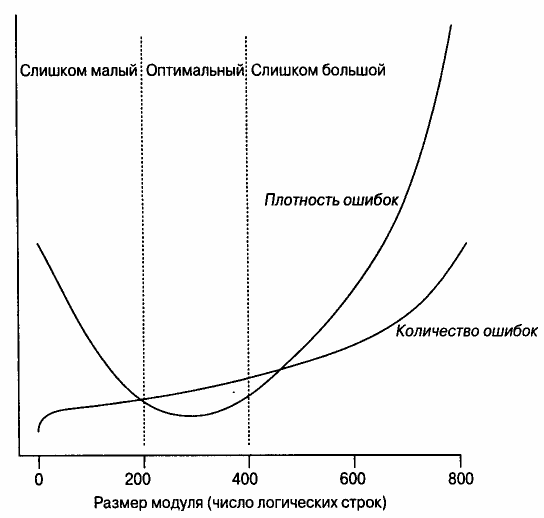
\includegraphics[width=200px]{../../slides/intro/errors_density-graph.png}
	\end{center}
\end{frame}

\begin{frame}{2. Правило ясности}
	\begin{block}{Ясность -- лучше чем мастерство.}
		Последующее обслуживание программы -- важная и дорогостоящая часть жизненного цикла программы.
	\end{block}
	\pause
Писать программы необходимо так,  как если бы вы знали,  что последующей поддержкой будет заниматься неуравновешенный псих с топором,  знающий ваш домашний адрес!
\end{frame}

\begin{frame}{3. Правило композиции}
	\begin{block}{Следует разрабатывать программы,  которые будут взаимодействовать с другими программами.}
		Если разрабатываемые программы не способны взаимодействовать друг с другом,  то очень трудно избежать создания сложных монолитных  программ.
	\end{block}
	Методы взаимодействия могут быть сильными и слабыми -- по возможности рекомендуется использовать слабые методы и текстовые форматы передачи данных.
\end{frame}

\begin{frame}{4. Правило разделения}
	\begin{block}{Следует отделять политику от механизма и интерфейсы от основных модулей (engine).}
		Примеры политики и механизма:\\
		вид GUI и операции отрисовки, клиент (front-end) -- сервер (back-end), сценарии и библиотеки и др.
	\end{block}
	При жесткой связи политики и механизма:
	\begin{itemize}
		\item политика становится негибкой и усложняется ее изменение;
		\item изменение политики имеет строгую тенденцию к дестабилизации механизмов.
	\end{itemize}
\end{frame}

\begin{frame}{5. Правило простоты}
	\begin{block}{Необходимо проектировать простые программы и <<добавлять сложность>> только там,  где это необходимо.}
	\end{block}
	Основные причины добавления сложности:
	\begin{itemize}
		\item человеческий фактор (часто -- желание <<выпендриться>>);
		\item проектные требования,  продиктованные текущей модой,  маркетингом или «левой пяткой заказчика»;
	\end{itemize}
\end{frame}

\begin{frame}{6. Правило расчетливости}
	\begin{block}{Пишите большие программы,  только если после демонстрации становится ясно,  что ничего другого не остается.}
		Под <<большими программами>> здесь понимаются программы с большим объемом кода и значительной внутренней сложностью.
	\end{block}
\end{frame}

\begin{frame}{7. Правило прозрачности}
	\begin{block}{Для того,  чтобы упростить проверку и отладку программы,  ее конструкция должна быть обозримой.}
		Программа {\itshape прозрачна}, если при ее минимальном изучении можно понять, что она делает и как.\\
		Программа {\itshape воспринимаема},  когда она имеет средства для мониторинга и отображения внутреннего состояния.
	\end{block}
	Необходимо использовать достаточно простые форматы входных и выходных данных.\\
	Интерфейс должен быть приспособлен для использования в отладочных сценариях.
\end{frame}

\begin{frame}{8. Правило устойчивости}
	\begin{block}{Устойчивость -- следствие	прозрачности и простоты.}
		Программа является {\itshape устойчивой},  когда она выполняет свои функции в неожиданных условиях,  которые выходят за рамки предположений разработчика,  как и в нормальных условиях.\\
		Программа является {\itshape простой},  если происходящее в ней не представляется сложным для восприятия человеком.
	\end{block}
	Один из способов организации -- модульность(простые блоки,  ясные интерфейсы)\\
	Следует избегать частных случаев!
\end{frame}

\begin{frame}{Пример неусточивого ПО}
	\begin{center}
		
\includegraphics[width=1\textwidth]{../../slides/intro/exploits_of_a_mom_rus.png}
	\end{center}
\end{frame}


\begin{frame}[fragile]{Пример <<простой>> программы}
	\begin{center}
		\begin{verbatim}
+++++++++++++++++++++++++++++++++++++++++++++
+++++++++++++++++++++++++++.+++++++++++++++++
++++++++++++.+++++++..+++.-------------------
---------------------------------------------
---------------.+++++++++++++++++++++++++++++
++++++++++++++++++++++++++.++++++++++++++++++
++++++.+++.------.--------.------------------
---------------------------------------------
----.-----------------------.
		\end{verbatim}
	\end{center}
\end{frame}

\begin{frame}{9. Правило представления}
	\begin{block}{Знания следует оставлять в данных,  чтобы логика программы могла быть примитивной и устойчивой.}
		Даже простую логику бывает сложно проверить,  но даже сложные структуры данных являются довольно простыми для моделирования и анализа (например диаграмма 50 узлов дерева и блок-схема 50 строк кода)
	\end{block}
	Если можно выбирать между усложнением структуры данных и усложнением кода,  то лучше выбирать первое.\\
	Примеры: ascii,  генератор html-таблицы.
\end{frame}

\begin{frame}{10. Правило наименьшего удивления}
	\begin{block}{При проектировании интерфейсов всегда следует использовать наименее неожиданные элементы.}
		Необходимо учитывать характер предполагаемой аудитории и традиции платформы.
	\end{block}
	Оборотная сторона: следует избегать создания внешне похожих вещей,  слегка отличающихся в действительности,  поскольку {\itshape кажущаяся привычность порождает ложные ожидания}.
\end{frame}

\begin{frame}{11. Правило тишины}
	\begin{block}{Если программе нечего сказать,  то пусть лучше молчит.}
		Внимание и сосредоточенность пользователя -- ценный и ограниченный ресурс,  который требуется только в случае необходимости.
	\end{block}
	Важная информация не должна смешиваться с подробными сведениями о работе программы.
\end{frame}

\begin{frame}{12. Правило восстановления}
	\begin{block}{Когда программа завершается аварийно,  это должно происходить явно (шумно) и по возможности быстро.}
		Если программа не способна справиться с ошибкой,  то необходимо завершить ее работу так,  чтобы максимально упростить диагностику.
	\end{block}
	Для сетевых служб следует следовать рекомендации Постела:\\
	<<{\itshape Будьте либеральны к тому,  что принимаете,  и консервативны к тому,  что отправляете}>>
\end{frame}

\begin{frame}{13. Правило экономии}
	\begin{block}{Время программиста дорого -- поэтому задача экономии его времени более приоритетна,  по сравнению с экономией машинного времени.}
		Компьютер железный -- ему не скучно (с) программистская мудрость
	\end{block}
	Использование высокоуровневых языков и <<обучение>> машины выполнять больше низкоуровневой работы по программированию,  что приводит к правилу 14.
\end{frame}

\begin{frame}{14. Правило генерации}
	\begin{block}{Избегайте кодирования вручную; если есть возможность -- пишите программы для создания программ.}
		Использование генераторов кода оправданно,  когда они могут повысить уровень абстракции,  
		т.е. когда язык спецификации для генератора проще,  чем сгенерированный код,  
		и код впоследствии не потребует ручной доработки.
	\end{block}
	Примеры: грамматические и лексические анализаторы,  генераторы make-файлов,  построители GUI-интерфейсов.
\end{frame}

\begin{frame}{15. Правило оптимизации}
	\begin{block}{Сначала -- опытный образец,  потом -- оптимизирование.}
		Добейтесь стабильной работы,  только потом оптимизируйте.
	\end{block}
	\begin{block}{Керниган и Плоджер:}
		90\% актуальной и реальной функциональности лучше,  чем 100\% функциональности перспективной и сомнительной
	\end{block}
	\begin{block}{Кнут:}
		преждевременная оптимизация -- корень всех зол
	\end{block}
	\begin{block}{Кент Бек (экстремальное программирование):}
		заставьте программу работать,  заставьте работать ее верно,  а затем сделайте ее быстрой
	\end{block}
\end{frame}

\begin{frame}{16. Правило разнообразия}
	\begin{block}{Не следует доверять утверждениям о <<единственно правильном пути>>.}
		Никто не обладает умом,  достаточым для оптимизации всего или для предвидения всех возможных вариантов использования создаваемой программы.
	\end{block}
\end{frame}

\begin{frame}{17. Правило расширяемости}
	\begin{block}{Разрабатывайте для будущего. Оно наступит быстрее,  чем вы думаете.}
		При проектировании протоколов или форматов файлов следует делать их самоописательными,  для того,  чтобы их можно было расширить.
	\end{block}
	{\itshape Всегда},  следует либо включать номер версии,  либо составлять формат из самодостаточных,  
	самоописательных команд так,  чтобы можно было легко добавить новые директивы,  
	а старые удалить, <<не сбивая с толку>> код чтения формата.
\end{frame}

\begin{frame}{Все правила сразу}
	\begin{center}
	{\Huge\bfseries K.I.S.S.}

	Keep It Simple,  Stupid!
	\end{center}
\end{frame}


}

\section{Дистрибутивы ОС Linux}

\mode<all>{\begin{frame}{Дистрибутив ОС GNU/Linux}
	\begin{block}{ Определение}
		\only<1>{\center{\bf{?}}}
		\pause
		\only<2->{Набор программного обеспечения на базе ядра Linux, распространяющийся как единое целое.}
	\end{block}
\end{frame}


\begin{frame}{Задачи дистрибутива}
	\begin{itemize}
		\item Предоставление комплекта ПО (ядро + утилиты)
		\item Средства установки и настройки
		\item Средства обновления
	\end{itemize}
\end{frame}

\begin{frame}{Различия между дистрибутивами}

	\only<1>{\Large\center{\bf{?}}}
	\pause
	\only<2->{\Large\center{\bf{Цели!!!}}}

	\bigskip
	\normalsize

	\pause

	\begin{itemize}
		\begin{columns}
		\column{0.4\textwidth}
			\item Инсталлятор
			\item Первичные настройки
			\item Средства управления
			\item Набор ПО
		\column{0.4\textwidth}
			\item Менеджер пакетов
			\item Формат распространения ПО
			\item Пути к файлам
			\item Система сборки ПО
		\end{columns}
	\end{itemize}
\end{frame}

\begin{frame}{Дистрибутивы}
	\begin{itemize}
		\begin{columns}
		\column{0.3\textwidth}
			\item RedHat
			\item Fedora Core
			\item CentOS
			\item Scientific Linux
			\item Oracle Unbreakable Linux
		\column{0.3\textwidth}
			\item Slackware 
			\item Gentoo
			\item Arch
			\item OpenSUSE
			\item ALT Linux 
		\column{0.3\textwidth}
			\item Debian
			\item Ubuntu
			\item Mint
			\item Knoppix
			\item BackTrack
		\end{columns}
	\end{itemize}
\end{frame}
}

\section{Процесс загрузки ОС Linux}

\subsection{Этапы загрузки}

\mode<all>{\begin{frame}{Процесс загрузки GNU/Linux}
	\small
	\begin{enumerate}
		\item BIOS
		\item MBR
			\pause
		\item Загрузка загрузчика
		\begin{itemize}
		\scriptsize
			\item Stage 1 -- Первичный загрузчик
			\item Stage 1,5 -- Загрузка ядра загрузчика и драйвера ФС
			\item Stage 2 -- Чтение конфигурации
		\end{itemize}
			\pause

		\item Загрузка ядра в память
		\item Загрузка initrd в память
			\pause
		\item Передача управления ядру
		\begin{itemize}
		\scriptsize
			\item Распаковка
			\item Инициализация
		\end{itemize}

		\item Монтирование initrd
		\item Запуск программы инициализации в initrd
			\pause
		\item Нахождение и монтирование корневого раздела
			\pause
		\item Запуск программы init
		\begin{itemize}
		\scriptsize
			\item Монтирование оставшихся разделов ФС
			\item Инициализация оборудования
			\item Запуск демонов
		\end{itemize}

	\end{enumerate}
\end{frame}


\begin{frame}{Наиболее распространенные загрузчики}
	\begin{itemize}
		\item GRUB
		\item LILO
		\item syslinux (isolinux, pxelinux)
		\item u-boot
	\end{itemize}
\end{frame}
}

\subsection{Ядро Linux}

\mode<all>{\begin{frame}{Задачи ядра Linux}
	\begin{itemize}
		\item Инициализация системы
		\item Управление процессами и потоками
		\item Управление памятью
		\item Управление файлами
		\item IPC
		\item Разграничение доступа
		\item Сетевые возможности
		\item Интерфейс доступа к возможностям ядра
	\end{itemize}
\end{frame}


\begin{frame}{Ядро}

	Ядро ОС Linux является модульным. 

	\begin{block}{Модули}
		\begin{itemize}
			\item В виде отдельных файлов
			\item "Вкомпилированные" в ядро
		\end{itemize}
	\end{block}

	\bigskip

	Список загруженных модулей: {\tt /proc/modules}
\end{frame}


\begin{frame}{Параметры ядра}
	
	Полный список: {\tt Documentation/kernel-parameters.txt}

	\begin{block}{Некоторые часто применяемые параметры}
		\begin{itemize}
			\begin{columns}
			\column{0.3\textwidth}
				\item console=ttyS0,9600
				\item debug
				\item init=/sbin/init
				\item loglevel=[0-7]
				\item maxcpus=[num]
			\column{0.3\textwidth}
				\item mem=nn[KMG]
				\item noacpi
				\item noapic
				\item panic=nn (sec)
				\item resume=/dev/sda2
			\column{0.3\textwidth}
				\item ro
				\item rw
				\item root=/dev/sda1
				\item rootdelay=nn (sec)
				\item rootwait
				\item vga=<num>|ask
			\end{columns}
		\end{itemize}
	\end{block}

	Модулям можно передавать параметры используя синтаксис: {\tt module.param=value}

	Параметры переданные ядру во время загрузки: {\tt /proc/cmdline}
\end{frame}

\begin{frame}{Магия SysRq}

	{\tt CONFIG\_MAGIC\_SYSRQ=y}

	{\tt /proc/sysrq-trigger}

	\begin{block}{{\bf R}eboot {\bf E}ven {\bf I}f {\bf S}ystem {\bf U}tterly {\bf B}roken}
		{\bf Ctrl+Alt+SysRq+?}

		\begin{itemize}
			\item h -- вывести список сочетаний на консоль
			\item b -- перезагрузка
			\item o -- выключение
			\item e -- послать сигнал SIGTERM всем процессам кроме init
			\item i -- послать сигнал SIGKILL всем процессам кроме init
			\item s -- синхронизировать все ФС 
			\item u -- переподключить все ФС в режиме RO
		\end{itemize}
		
	\end{block}


\end{frame}
}

\subsection{Userspace}

\mode<all>{\input{../../slides/intro/initrd}}

\mode<all>{\begin{frame}{init}
	Менеджер управления работой системой и сервисами.
	
	\bigskip

	\center{\large PID = 1}

	\bigskip

	\begin{block}{Наиболее известные}
		\begin{itemize}
			\item SysVInit
			\item systemd
			\item upstart
		\end{itemize}
	\end{block}
\end{frame}

\begin{frame}{SysVInit}
	\begin{block}{Управление}
		\begin{itemize}
			\item kernel boot parameters: <N> -- runlevel
			\item утилита {\tt runlevel}
			\item утилита {\tt init}
		\end{itemize}
	\end{block}

	\scriptsize
	\begin{block}{Runlevel}
		\begin{table}
			\begin{tabular}{| c | l | }
			\hline
			Runlevel & Описание\\
			\hline
			0	& Выключить систему \\
			1,s,single & Однопользовательский режим \\
			2	& Многопользовательский режим без графики. Без сетевых сервисов.\\
			3	& Многопользовательский режим без графики. Полноценная сеть. \\
			4	& Определяется на хосте\\
			5	& Многопользовательский режим с графикой.\\
			6	& Перезагрузка\\
			emergency & Аварийная оболочка \\
			\hline
			\end{tabular}
		\end{table}
	\end{block}
\end{frame}

\begin{frame}{SysVInit: сервисы}
	\begin{block}{Управление}
		\begin{itemize}
			\item утилита {\tt service}
			\item утилита {\tt chkconfig}
		\end{itemize}
	\end{block}

	\begin{block}{Сервисы}
		\begin{itemize}
			\item {\tt /etc/rc.d/init.d}
			\item {\tt /etc/rc.d/rc.N}\footnote{N=runlevel}
		\end{itemize}
	\end{block}
\end{frame}

\begin{frame}{systemd}
	\begin{block}{Управление}
		\begin{itemize}
			\item kernel boot parameters\\
				{\tt systemd.unit=rescue.target} \\
			\item утилита {\tt systemctl} \\
				{\tt systemctl isolate multi-user.target} \\
				{\tt systemctl set-default single.target}
		\end{itemize}
	\end{block}

	\begin{block}{targets}
		\tiny
		\begin{table}
			\begin{tabular}{| c | l | l | }
			\hline
			Runlevel & Описание\\
			\hline
			0	& poweroff.target & Выключить систему \\
			1,s,single & rescue.target  & Однопользовательский режим \\
			2	& multi-user.target & Многопользовательский режим без графики. Без сетевых сервисов.\\
			3	& multi-user.target & Многопользовательский режим без графики. Полноценная сеть. \\
			4	& multi-user.target & Определяется на хосте\\
			5	& graphical.target & Многопользовательский режим с графикой.\\
			6	& reboot.target & Перезагрузка\\
			emergency & emergency.target & Аварийная оболочка \\
			\hline
			\end{tabular}
		\end{table}
	\end{block}
\end{frame}

\begin{frame}{systemd: сервисы}
	\begin{block}{Управление}
		\begin{itemize}
			\item утилита {\tt systemctl}
		\end{itemize}
	\end{block}

	\begin{block}{Сервисы}
		\begin{itemize}
			\item {\tt /lib/systemd/system/}
			\item {\tt /etc/systemd/system/}
		\end{itemize}
	\end{block}
\end{frame}
}

\subsection{Практика}

\mode<all>{\begin{frame}{Практическое задание}
	\begin{enumerate}
		\item Загрузить ОС по умолчанию
		\item Посмотреть используемые параметры ядра 
		\item Посмотреть список загруженных модулей
			\pause
		\item Переопределить init на sh
		\item SysRq. {\bf R}eboot {\bf E}ven {\bf I}f {\bf S}ystem {\bf U}tterly {\bf B}roken
			\pause
		\item Загрузить ядро с "урезанным" количеством памяти
		\item Отключить 1 или несколько процессоров
			\pause
		\item Посмотреть текущий runlevel
		\item Посмотреть список сервисов
	\end{enumerate}
\end{frame}
}


\chapter{Командная строка}

\section{Интерфейс командной строки}
\mode<all>{% Тема. Командная строка. 
% Показать примеры использования. Рассказать о преимуществах и недостатках в
% сравненни с графическим "оконным" интерфейсом. 
% Ознакомить с назначениме  эмулятора терминала и об реализациях.

\begin{frame}{Примеры использования командной строки}
	\begin{columns}
	\column{0.5\textwidth}
        \begin{itemize}
            \item чаты
            \item компьютерные игры Quake, DotA
            \item операционные системы
        \end{itemize}
	\column{0.5\textwidth}
	% insert picture of Quake 
    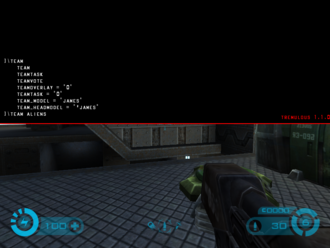
\includegraphics[height=0.4\textheight]{../../slides/cmdline/330px-Tremulous_console.png}
	\end{columns}
\end{frame}

\begin{frame}{Преимущества командной строки}
	\begin{itemize}
		\item Работа через сеть либо RS232
		\item Быстрый доступ к командам системы
		\item Легче отладка сообществом
		\item Легкость автоматизации
	\end{itemize}
\end{frame}

\begin{frame}{Недостатки командной строки}
	\begin{itemize}
		\item Oтсутствуют возможности обнаружения (discoverabililty)
		\item Необходимость изучения синтаксиса команд и запоминания сокращений.  (синтаксис может различаться)
		\item Без автодополнения, ввод длинных и содержащих спецсимволы параметров с клавиатуры может быть затруднительным
		\item Отсутствие «аналогового» ввода.
	\end{itemize}
\end{frame}

\begin{frame}{Эмуляторы терминала в графическом режиме}
	\begin{itemize}
		\item xterm
		\item rxvt
        \item gnome-terminal
        \item konsole
        \item Yakuake (Yet Another Kuake)
	\end{itemize}
\end{frame}
\note { 
Примеры приложений которые лучше выглядят в графическом режиме браузер,
редакторы видео и графики. Поэтому пользователь при работе, как правило,
совмещает оба интерфейса: использует графическое окружениe в сочетании с
интерфейсом командной строки. 
В графическом окружении интерфейса командной строки предоставляют приложения -
эмуляторы терминала. 
реализации - для графической системы X Window xterm, rxvt. Для GNOME
gnome-terminal, для KDE konsole, Yakuake (Yet Another Kuake выезжает по нажатии
тильды ~ как Quake)  
Дополнительные замечания:
Терминал - устройство для ввода вывода информации, уже устарел.
Графические приложения можно запускать из командной строки. 
}
}

\section{Командная оболочка (shell)}

\mode<all>{\begin{frame}[fragile]{Определение(не совсем формальное)}
	\textbf{Shell} -- приложение, обеспечивающее выполнение других приложений и их взаимодействие, а также представляющая услуги командной строки. 
	\begin{center}
	 или
	\end{center}
	\textbf{Shell} -- приложение, обеспечивающее доступ к основным функциям ядра.

	\pause
	\vspace{0.5in}
	Пример shell из Windows-world -- cmd.exe
	\vspace{0.5in}

	Минимальный дистрибутив Linux -- ядро + shell 

\end{frame}

\begin{frame}[fragile]{Основные типы shell в Unix}
  \begin{itemize}
    \item Bourne shell совместимые
      \begin{itemize}
        \item \textbf{sh} исходная bourne shell (Steve Bourne, 1978)
        \item \textbf{ksh} Korn shell (David Korn, 1983)
        \item \textbf{ash} $[$BSD$]$ Almquist shell (Kenneth Almquist,1989)  
        \item \textbf{bash} $[$GPL$]$ Bourne-again shell (Brian Fox, 1989)
        \item \textbf{zsh} $[$BSD$]$ Z shell (Paul Falstad,1990)
        \item \textbf{/bin/sh} Указывает на POSIX-совместимую shell
      \end{itemize}
  \item C shell совместимые
      \begin{itemize}
        \item \textbf{csh}  Исходная С shell (Bill Joy, 1978)
        \item \textbf{tcsh} $[$BSD$]$ TENEX C shell (Ken Greer, 1981)
       \end{itemize}
  \end{itemize}
\end{frame}

\begin{frame}[fragile]{Маленькое упражнение}
\begin{lstlisting}[language=bash]
cat /etc/shells
ls -l <filename> # для каждого элемента /etc/shells
readlink -e <filename> 
\end{lstlisting}
\end{frame}


}

\section{Don't panic! Получение помощи}

\mode<all>{
\begin{frame}[fragile]{Как правильно задавать вопросы}
From FAQ How To Ask Questions The Smart Way
Before You Ask
  \begin{itemize}
	  \item Try to find an answer by reading the manual.
	  \item Try to find an answer by reading a FAQ.
	  \item Try to find an answer by searching the archives of the forum you plan to post to.
	  \item Try to find an answer by searching the Web.
	  \item Try to find an answer by inspection or experimentation.
	  \item Try to find an answer by asking a skilled friend.
	  \item If you're a programmer, try to find an answer by reading the source code.
    \end{itemize}
\end{frame}


\begin{frame}[fragile]{Источники получение помощи}
  \begin{itemize}
    \pause
    \item \textbf{man} - помощь по внешним командам
    \pause
    \item \textbf{help} - встроенная помощь по внутренним командам bash (также man bash)
    \pause
    \item \textbf{info} - расширенная помощь по некоторым командам (texinfo format)
     \begin{block}{Упражнение. Работа с командой info}
        \begin{itemize}
        \item   Попробовать {\tt info coreutils}
        \item   Справка по навигации -- нажать h
        \end{itemize}
	 \end{block}
		\begin{block}{Упражнение. Другие источники помощи.}
			\begin{lstlisting}
            help 
            help help
            man -h
            info --help
			\end{lstlisting}
		\end{block}
  \end{itemize}
\end{frame}

\begin{frame}[fragile]{Основное о man}
\begin{columns}
	\column{2.5in}
		\begin{itemize}
			\item Прочитайте {\tt man man} !
			\item apropos, аналог {\tt man -k <слово>}
            \item whatis, аналог {\tt man -f <слово>} 
			\item Разделы (sections)
				\begin{itemize}
					\item[1] Основная секция(юзерские программы)
					\item[2] Syscalls
					\item[3] С library
					\item[5] Конфигурационные файлы
					\item[8] Системные службы
				\end{itemize}
		\end{itemize}
	  \textbf{Замечание}

	  Обычно внутри страницы работает поиск с помощью '/'
	\pause 
	
	\column{1in}
		\begin{block}{Попробовать}
			\begin{lstlisting}
man -k intro or apropos
man -f intro or whatis
man 3 intro
man 1 intro
man -wa intro
			\end{lstlisting}
		\end{block}
	\end{columns}
\end{frame}


%\begin{frame}[fragile]{Чему научились}
%  \begin{itemize}
%  \item Как спрашивать у сообщества
%  \item Умеем использовать 3 источника получения информации man, info, help
%  \item Как перемещаться по страницам помощи info и man
%  \item Иcкать в системе помощи man и запрашивать из одного из 8-ми разделов 
%  \end{itemize}
%\end{frame}
}

\section{Навигация по файловой системе}

\mode<all>{\begin{frame}{Навигация по файловой системе}
      \begin{itemize}
		  \item {\tt ls} -- список файлов в (текущей по умолчанию) директории (man ls)
		  \item {\tt cd} -- смена текущей директории (help cd)
		  \item {\tt pwd} -- имя текущей директории (help pwd)
      \end{itemize}
\end{frame}

\begin{frame}[fragile]{Команды для работы с файлами}
	\begin{itemize}
		\begin{columns}
		\column{0.2\textwidth}
			\item touch
			\item ln
			\item mkdir
			\item mknod
			\item mkfifo
		\column{0.2\textwidth}
			\item cp
			\item mv
			\item install
			\item rm
			\item rmdir
			\item file
		\column{0.4\textwidth}
			\begin{block}{Упражнение}
				\begin{enumerate}
					\item Создать иерархию директорий
						\begin{lstlisting}
dir1/dir1.1/dir1.1.1
dir1/dir1.2/dir1.2.1
dir1/dir1.2/dir1.2.2
						\end{lstlisting}
					\item Внутри каждой создать файл
					\item Удалить все созданное
				\end{enumerate}
			\end{block}
		\end{columns}
	\end{itemize}
\end{frame}


}

\mode<all>{\begin{frame}{Файловая структура}
	
	{\center "Дерево внутри дома?" (c) Шрек}
		
	\begin{columns}
	\column{0.2\textwidth}
		\includegraphics[height=0.8\textheight]{../../slides/fs/01-lhs.png}
		
	\column{0.7\textwidth}
		\begin{itemize}
			\item Директории
			\item Обычные файлы
			\item Симлинки
			\item Хардлинки
			\item Файлы устройств
			\item FIFO
			\item сокеты
		\end{itemize}
	\end{columns}
\end{frame}
}

\section{Дополнительные возможности оболочки}
\mode<all>{\begin{frame}{Важные аббревиатуры внутри командной строки}
  \begin{itemize}
    \item Для директорий
      \begin{itemize}
        \item {\tt $\sim$} Домашняя директория
        \item {\tt $\sim$<username>} Домашняя директория пользователя
        \item {\tt ..} Родительская директория
        \item {\tt .} Текущая директория
      \end{itemize}
      \pause  
    \item Wildcards
      \begin{itemize}
        \item {\tt *} Любой набор символов {\tt file*txt : file1.txt filefilefiletxt}
        \item {\tt $[$<список>$]$ } символ из заданного набора
        \item {\tt ?} любой один символ
      \end{itemize}

  \end{itemize}
\end{frame}       

\begin{frame}{Горячие клавиши}
  \begin{itemize}
    \item \textbf{Tab} -- дополнение текущей команды
      \pause
    \item История команд
      \begin{itemize}
        \item Клавиши курсора -- навигация по истории
        \item Ctrl-R -- поиск в истории по фрагменту
        \item Ctrl-O (после выполнения вставить следующую команду из истории)
        \item Команда {\tt history}
      \end{itemize}
    \item Навигация

  \end{itemize}
\end{frame}

\begin{frame}{Переменные окружения}
  \begin{itemize}
    \item {\tt HOME}
    \item {\tt PWD}
    \item {\tt LANG}
    \item {\tt LD\_LIBRARY\_PATH}
    \item {\tt SHELL}
    \item {\tt TERM}
    \item {\tt DISPLAY}
  \end{itemize}

  Контроль

  \begin{itemize}
    \item export {\tt export VAR=value}
    \item declare -x
    \item echo 
  \end{itemize}

  Переменные окружения наследуются при создании нового процесса
\end{frame}

%\begin{frame}{Настройки bash и кастомизация}
%  \begin{itemize}
%    \item Login shell
%      \begin{itemize}
%        \item {\tt /etc/profile}
%        \item {\tt $\sim$/.profile }
%      \end{itemize}
%    \item Обычная интерактивная shell
%      \begin{itemize}
%        \item {\tt /etc/bash.bashrc}
%        \item {\tt $\sim$/.bashrc}
%      \end{itemize}
%  \end{itemize}
%
%  Полезные команды
%  \begin{itemize}
%    \item {\tt alias}
%    \item {\tt export PATH=}
%    \item {\tt Определение функции}
%    \item {\tt shopts}
%  \end{itemize}
%
%\end{frame}


}

\section{Процессы}
\mode<all>{\begin{frame}{Процессы в UNIX}
  \begin{itemize}
    \item Создание процессов
      \begin{itemize}
        \item fork
        \item exec
      \end{itemize}
    \item Атрибуты процесса
      \begin{itemize}
        \item pid 
        \item файловые дескрипторы
        \item environment
        \item Рабочая директория (cwd)
        \item прочее в директории {\tt /proc/<pid>}
      \end{itemize}
  \end{itemize}
\end{frame}

\begin{frame}{Управление процессами}
  \begin{itemize}
    \item kill (killall)
    \item top
    \item pstree
    \item Команды управления процессами в bash: 
      \begin{itemize}
        \item {\tt jobs}, {\tt fg, \tt bg}
        \item Ctrl-C -- оборвать выполнение процесса (SIGINT)
        \item Ctrl-Z -- остановить выполнение команды (SIGTSTP)
        \item Ctrl-D -- завершить ввод
      \end{itemize}
  \end{itemize}
\end{frame}


\begin{frame}{Упражнения}
  \begin{block}{Посмотреть вывод pstree}
    {\tt pstree}
  \end{block}
  \pause
  \begin{block}{Ctrl-C, Ctrl-Z}
    В графическом режиме запустить из терминала emacs

    Ctrl-Z

    jobs -l

    bg +
  \end{block}
  \pause
  \begin{block}{fork bomb}

    {\tt ulimit -u 200} 

    {\tt bomb()\{ (bomb; bomb) \& \} }

    top

    killall bash

  \end{block}
\end{frame}


\begin{frame}{Unix way}
  \begin{enumerate}
    \item Пишите программы, которые делают одну вещь и делают её хорошо.
    \item Пишите программы, которые бы работали вместе.
    \item Пишите программы, которые бы поддерживали текстовые потоки, поскольку это универсальный интерфейс. 
  \end{enumerate}
\end{frame}

\begin{frame}{Unix way}
  \begin{enumerate}
    \item   Маленькое прекрасно.
    \item   Пусть каждая программа делает одну вещь, но хорошо.
    \item   Собирайте прототип как можно раньше.
    \item   Предпочитайте переносимость эффективности.
    \item   Храните данные в простых текстовых файлах.
    \item   Используйте программные рычаги для достижения цели.
    \item   Используйте сценарии командной строки для улучшения функционала и переносимости.
    \item   Избегайте <<связывающего>> (captive) пользовательского интерфейса.
    \item   Делайте каждую программу «фильтром».
  \end{enumerate}
\end{frame}

\begin{frame}{Конвееры}
%  \textbf{Цель} -- максимальная модульность: большое количество простых приложений, взаимодействующих друг с другом для решения задач
  \only<1>{
  \begin{center}
    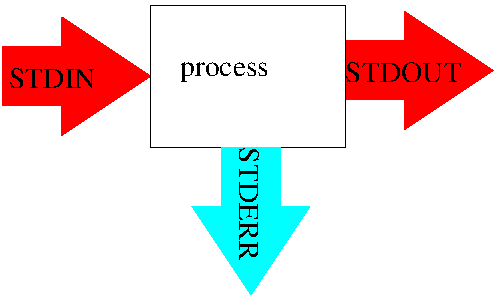
\includegraphics[width=1.2in]{../../slides/cmdline/process}
  \end{center}
  }
  \only<2>{
    \begin{center}
      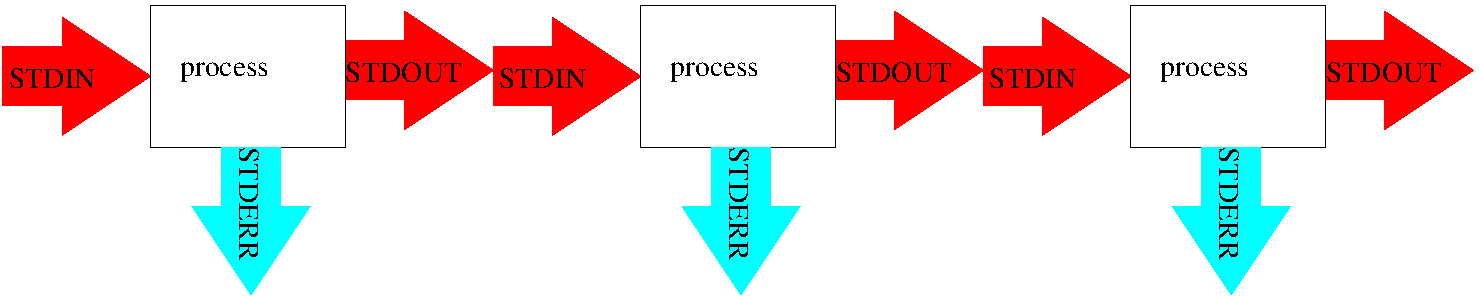
\includegraphics[width=3.6in]{../../slides/cmdline/processes}
    \end{center}
  }
  \begin{itemize}
    \item <1-> Каждое приложение открывает 3 стандартных файловых дескриптора stdin (fd 0), stdout(fd 1), stderr (fd 2)
    \item <2-> Приложения могут работать как фильтр из STDIN в STDOUT, можно объединять несколько приложений в конвейер
    \item <2-> Синтаксис {\tt <app1> | <app2>}
  \end{itemize}
\end{frame}
}

\section{Перенаправление ввода-вывода}
\mode<all>{

\begin{frame}{Конвееры}
%  \textbf{Цель} -- максимальная модульность: большое количество простых приложений, взаимодействующих друг с другом для решения задач
  \only<1>{
  \begin{center}
    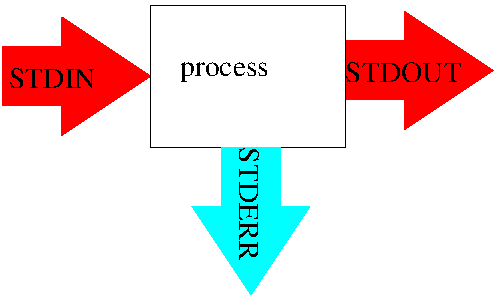
\includegraphics[width=1.2in]{../../slides/cmdline/process}
  \end{center}
  }
  \only<2>{
    \begin{center}
      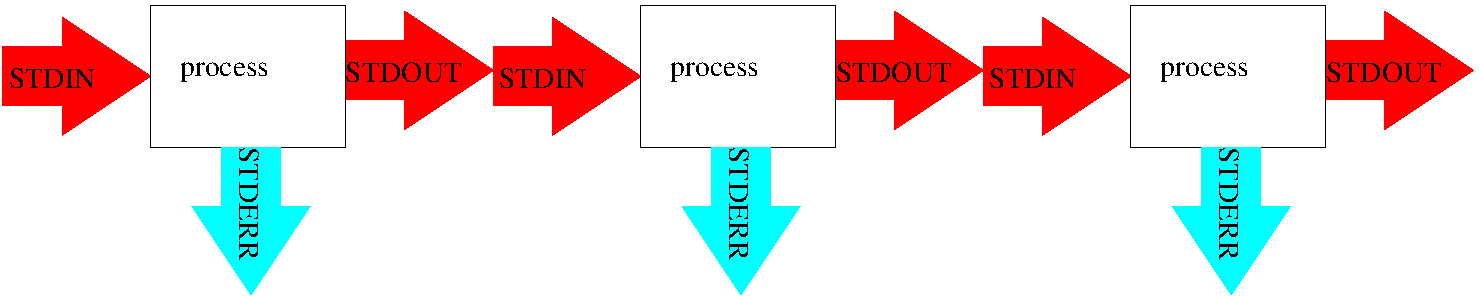
\includegraphics[width=3.6in]{../../slides/cmdline/processes}
    \end{center}
  }
  \begin{itemize}
    \item <1-> Каждое приложение открывает 3 стандартных файловых дескриптора stdin (fd 0), stdout(fd 1), stderr (fd 2)
    \item <2-> Приложения могут работать как фильтр из STDIN в STDOUT, можно объединять несколько приложений в конвейер
    \item <2-> Синтаксис {\tt <app1> | <app2>}
  \end{itemize}
\end{frame}
}
\mode<all>{\begin{frame}{Перенаправления в файл}

\begin{itemize}
  \item Перенаправление stdout 
    \begin{itemize}
      \item С созданием нового файла

        {\tt command > file}\\
		Например {\tt cat file1 file2 > file3}
      \item С дополнением существующего

		  {\tt command >\phantom{}>  file}
    \end{itemize}
    \pause
  \item Перенаправления stdin

    {\tt command < file}
    \pause
  \item Перенаправления stderr

    {\tt command1 2>\&1 | command2}

   {\tt command 1>file 2>\&1}

   {\tt command 2>file 1>\&2}
\end{itemize}

\end{frame}


}
\mode<all>{\begin{frame}[fragile]{Мультистрочный ввод (Here-документ)}

\begin{verbatim}
program <<LABEL
Тут
    много
	     строк
LABEL
\end{verbatim}

	\pause
	\begin{block}{Пример}
	Передадим несколько строк в COM-порт 1
\begin{lstlisting}[language=bash]
cat >/dev/ttyS0 <<E_O_F
ATZ
ATDT 8w0170123456
E_O_F
\end{lstlisting}
	\end{block}
\end{frame}
}

\section{Полезные команды}

\mode<all>{\begin{frame}{Дополнительный набор команд}
  \begin{itemize}
    \item {\tt cat} - Вывод файла в stdout, соединение нескольких файлов в stdout
    \item {\tt wc} - подсчет статистики символов в файле или в stdin 
    \item {\tt sort} - сортировка строк файла
    \item {\tt uniq} - объединение одинаковых строк в одну
    \item {\tt tr} - замена набора символов
    \item {\tt less} - программа-пейджер
    \item {\tt grep} - поиск строк, соответствующих регулярному выражению
    \item {\tt cut} - выделение полей из строк stdin
    \item {\tt awk} - небольшой язык программирования (также полезен для выделения полей)
  \end{itemize}
\end{frame}

\begin{frame}[fragile]{Некоторые примеры использования}
\begin{lstlisting}[language=bash]
cat /proc/1/environ | tr '\0' '\n' | less
ls  | wc -l # подсчет числа файлов
man uniq | tr  '[:space:]' '\n' | sort | uniq -c | sort -n | less # подсчет количества слов в тексте man uniq
history | wc -l # подсчет ранее введенных команд
cat /etc/udev/rules.d/* | wc -l
ls -s *.jpg | awk 'BEGIN{s=0};/^[ ]*[0-9]/{s+=\$1};END{print s}' 
\end{lstlisting}
  \pause
  \begin{block}{Упражнение}
    Посчитать статистику использования команд в history
  \end{block}
\end{frame}

\begin{frame}{Дополнительный набор команд для работы с текстом}
	\begin{itemize}
	  \item {\tt head} -- вывести первые строки
	  \item {\tt tail} -- вывести последние строки
		\begin{itemize}
			\item {\tt -f} -- отслеживать добавление данных в файл 
		\end{itemize}
	  \item {\tt tee} -- копировать стандартный вывод в файл
	  \item {\tt grep} -- печать текста, соответствующего шаблону
		\begin{itemize}
			\item {\tt -i}	
			\item {\tt -v}
			\item {\tt -o}
		\end{itemize}
	\end{itemize}
\end{frame}

}

\subsection{Архиваторы}
\mode<all>{\begin{frame}[fragile]{Архивация}
	\begin{block}{Архивация: tar}
		\begin{itemize}
			\item {\tt -c} -- создать архив
			\item {\tt -x} -- извлечь из архива
				\begin{itemize}
					\item {\tt -C} -- перейти в директорию
					\item {\tt -{}-strip-components=N} -- пропустить N уровней
				\end{itemize}
			\item {\tt -f} -- запись в файл
		\end{itemize}
	\end{block}

	\begin{block}{Сжатие: gzip, bzip, xz}
		\begin{itemize}
			\item {\tt -[1-9]} -- изменить уровень сжатия
			\item {\tt -d} -- распаковать
			\item {\tt -c} -- вывод на консоль
		\end{itemize}
		\begin{verbatim}
dd if=/dev/sda bs=1M count=1 | gzip -c > backup.gz
		\end{verbatim}
	\end{block}

\end{frame}

\begin{frame}[fragile]{Архивация: примеры}

	Создать сжатый архив:
	\begin{verbatim}
tar -czf archive.tar.gz *
	\end{verbatim}
	\pause
	Распаковать сжатый архив в директорию {\tt /tmp}:
	\begin{verbatim}
tar -C /tmp/ -xzf archive.tar.gz 
	\end{verbatim}
	\pause
	Создать сжатый архив:
	\begin{verbatim}
tar -czf archive.tar.gz *
	\end{verbatim}
	\pause
	Создать копию текущей директории в директории {\tt /tmp/copy/}:
	\begin{verbatim}
tar -c * | tar -C /tmp/copy -x
tar -cf - * | tar -C /tmp -xf -
	\end{verbatim}
	\pause
	Создать копию текущей директории на другом хосте:
	\begin{verbatim}
HostDest: netcat -l 2222 | gzip -dc | tar -C /tmp/copy/ -x
HostSrc:  tar -c * | gzip -9 | netcat HostDest 2222
	\end{verbatim}
\end{frame}
}

\subsection{find и xargs}
\mode<all>{\begin{frame}[fragile]{Поиск файлов}
	\begin{block}{find}
		\begin{itemize}
			\item {\tt -type} -- тип файлового объекта
			\item {\tt -size} -- размер
			\item {\tt -maxdepth} -- глубина рекурсии
			\item {\tt -exec} -- выполнить команду
			\item {\tt -printf} -- форматированный вывод
		\end{itemize}
	\end{block}

	\begin{block}{Примеры}
		\begin{verbatim}
find /etc -type f -size +100k  -exec ls -l {} \;
		\end{verbatim}

		\begin{verbatim}
find -type d -user altlinux
		\end{verbatim}
	
	\end{block}
\end{frame}

\begin{frame}[fragile]{xargs}
	\begin{block}{xargs}
			Утилита для создания и запуска команд из стандартного потока ввода:
		\begin{verbatim}
xargs [options] command [command options]
		\end{verbatim}

		\begin{itemize}
			\item {\tt -d} -- разделитель
			\item {\tt -0} -- null-terminated строки
			\item {\tt -I text} -- подстановка
			\item {\tt -n N} -- максимальное количество аргументов
			\item {\tt -P N} -- максимальное количество процессов
		\end{itemize}

	\end{block}
\end{frame}

\begin{frame}[fragile]{xargs}
	\begin{block}{Примеры}
		\begin{verbatim}
find /etc -type f -size -100k | xargs tar -czf /tmp/archive-100k.tar.gz
		\end{verbatim}

		\begin{verbatim}
find /etc -type f | xargs -I {} echo "Найден {} файл"
		\end{verbatim}

		\begin{verbatim}
find . -type f -name "*.mp3" -print0 | xargs -0 -n 1 -P 0 -I mp3 avconv -i mp3 mp3.ogg
		\end{verbatim}
	
	\end{block}
\end{frame}


}

\subsection{Редакторы}
\mode<all>{\begin{frame}{Редакторы}
	\begin{itemize}
		\item Интерактивные
			\begin{itemize}
				\item vi
					\begin{itemize}
						\item Есть почти везде
					\end{itemize}
				\item vim
				\item emacs
			\end{itemize}
		\item Поточные
			\begin{itemize}
				\item {\tt ed}
				\item {\tt sed}
				\item {\tt awk}
			\end{itemize}
	\end{itemize}
\end{frame}

\begin{frame}[fragile]{Метасимволы}
	\begin{block}{grep, sed, awk}
	\end{block}
	\begin{itemize}
		\item {\tt .} -- любой символ за исключением пустой строки
		\item {\tt *} -- любоe количество символов, которые стоят перед {\tt *}
		\item {\tt \^{}} -- начало строки
		\item {\tt \$} -- конец строки
		\item {\tt [...]} -- любой символ из заключенных в скобки
	\end{itemize}
\end{frame}

\begin{frame}[fragile]{sed}
	\begin{block}{Сценарии}
		{\tt [ addr [ ,  addr ] ] cmd [ args ]}
	\end{block}

	\tiny
	\begin{block}{Команды}
		\begin{itemize}
		  \item {\tt a, i} -- добавить строку после (перед) текущей
			  \begin{verbatim} who | sed -e 'a Text' \end{verbatim}
		  \item {\tt c} -- удалить строку и заменить на текст
			  \begin{verbatim} who | sed -e "/$USER/ c Юзверь" \end{verbatim}
		  \item {\tt d} -- удалить строку
			  \begin{verbatim} who | sed -e '2,4 d' \end{verbatim}
			  \begin{verbatim} who | sed -e '/pts/ d' \end{verbatim}
		  \item {\tt s} -- замена по регулярному выражению
			  \begin{verbatim} who | sed -e "s/$USER/Юзверь/g" \end{verbatim}
		\end{itemize}
	\end{block}
\end{frame}


}

\chapter{Система управления пакетами}
\section{Система управления пакетами}
\mode<all>{\begin{frame}
	\frametitle{И еще раз про "DLL hell"}
	
	\begin{block}{Устанавливаем программу}
	А что же с библиотеками?
	\end{block}

	\pause

	\begin{columns}
		\column{0.5\textwidth}
		\begin{block}{"В системе все есть!"}
		\begin{itemize}
			\item Oh, really???
			\item И нужной версии?
			\item А API и ABI точно не менялись?
			\item А если библиотек несколько версий?
			\item А если нужны дополнительные программы?
		\end{itemize}
		\end{block}
		\pause
		\column{0.5\textwidth}
		\begin{block}{"Всё своё, ношу с собой!"}
		\begin{itemize}
			\item А как насчет объема?
			\item Использование памяти.
			\item А что насчет лицензий?
			\item И все-таки порядок загрузки...
			\item Не спасает от проблем с 3rd-party ПО.
		\end{itemize}
		\end{block}
	\end{columns}
\end{frame}

\begin{frame}
	\frametitle{Хаос}

	\begin{center}
		"Даешь каждой платформе и языку собственную систему управления пакетами!"
	\end{center}

	\begin{block}{Увы, мы не в идеальном мире}
		\begin{itemize}
			\item Дистрибутивы: rpm\{4,5\}, deb, portage, pacman... и куча модификаций...
			\item Дополнительный софт: {\tt ./configure; make; make install}
			\item Java: {\tt ivy, ant, maven, gradle}
			\item Ruby: gem
			\item Perl: CPAN
			\item Python: pip + PyPi
		\end{itemize}
	\end{block}

\end{frame}

\begin{frame}
	\frametitle{Разработка и использование в реальной системе}
	
	\begin{block}{Build-time vs Run-time}

		\begin{enumerate}
			\item Не все, что нужно во время компиляции, должно быть установлено в конечной системе.
			\item Не все, что нужно для работы программы, необходимо устанавливать на сборочной системе.
		\end{enumerate}
	\end{block}
%TODO перенести после описания структуры каталогов
	\begin{block}{Чистое сборочное окружение}
		\begin{itemize}
			\item Воспроизводимость сборки 
			\item Контроль зависимостей
			\item Контроль автоматически "подхваченных" зависимостей
		\end{itemize}
	\end{block}
\end{frame}

}

\mode<all>{\begin{frame}{Система управления пакетами: для чего это нужно}
\begin{itemize}
 \item ''DLL Hell''
 \item Dependency hell
 \item Общие задачи пакетного менеджера:
   \begin{itemize}
     \item Проверка целостности пакетов
     \item Проверка зависимостей пакетов
        \item Поддержание списка установленных пакетов
        \item Автоматическое удаление пакетов
     \item Предоставление доступа к репозиторию пакетов
     \item Разрешение зависимостей
   \end{itemize}
\end{itemize}
\end{frame}

\begin{frame}{Debian-based и RedHat-based системы управления пакетами}
\begin{center}
 \textbf{Два уровня пакетных менеджеров}
\end{center}
\begin{columns}
  \column{0.4\textwidth}
  \begin{center}
    \textbf{RedHat-based}
  \end{center}
  \begin{itemize}
    \item dnf/yum
    \item rpm
  \end{itemize}
  \column{0.4\textwidth}
  \begin{center}
    \textbf{Debian-based}
  \end{center}
  \begin{itemize}
    \item aptitude, apt, synaptic
    \item dpkg
  \end{itemize}
\end{columns}
\end{frame}
}

\mode<all>{\begin{frame}{RPM: команды}
	\begin{block}{Установка пакета}
		{\tt rpm -i [rpm-file1] ... [[url://]rpm-fileN] }
	\end{block}
	\begin{block}{Удаление пакета}
		{\tt rpm -e pkgname1 ... pkgnameN }
	\end{block}
	\begin{block}{Обновление пакета}
		{\tt rpm -U [rpm-file1] ... [[url://]rpm-fileN] }
	\end{block}
	\begin{block}{Проверка пакета}
		{\tt rpm -V pkgname1 ... pkgnameN }
	\end{block}
\end{frame}

\begin{frame}{RPM: часто используемые опции опроса}

	\begin{itemize}
		\item {\tt pkgname} -- выбор пакета, установленного в системе
		\item {\tt -a} -- все пакеты, установленные в системе
		\item {\tt -p} -- использовать файл RPM
	\end{itemize}


	\begin{itemize}
		\item {\tt -i} -- показать информацию пакета\\
			{\tt rpm -q -i glibc }
		\item {\tt -l} -- показать список файлов пакета \\
			{\tt rpm -q -l glibc }
		\item {\tt --whatprovides} -- \\
			{\tt rpm -q --whatprovides java}
		\item {\tt --whatrequires} -- \\
			{\tt rpm -q --whatrequires /bin/bash}
		\item {\tt --queryformat} -- формат вывода\\
			{\tt rpm -q --whatrequires /bin/bash --queryformat ''\%\{name\} ''}

	\end{itemize}

\end{frame}


}

\mode<all>{\newcounter{tmpc}

\begin{frame}{Репозиторий}
	\begin{block}{Репозиторий пакетов}
		Место, где хранятся и поддерживаются пакеты, а также сопутствующая мета-информация, предназначенное для использования пакетным менеджером.
	\end{block}
	\begin{block}{Пример: Fedora Core}
		\begin{itemize}
			\item Packages/*.rpm
			\item RPM-GPG-KEY-*
			\item repodata
			\begin{itemize}
				\item множество сжатых и несжатых XML файлов для YUM
			\end{itemize}
		\end{itemize}

		Описание репозтория для YUM на локальной системе хранится по пути
		{\tt /etc/yum.repos.d/*.repo}
	\end{block}
		
\end{frame}

\begin{frame}{YUM: команды}
	\begin{block}{Установка/обновление пакета}
		{\tt yum install pkgname }
	\end{block}
	\begin{block}{Обновление всех пакетов}
		{\tt yum update }
	\end{block}
	\begin{block}{Удаление пакета}
		{\tt yum remove pkgname }
	\end{block}
	\begin{block}{Поиск}
		{\tt yum list pkgname }\\
		{\tt yum search pkgname }
	\end{block}
\end{frame}


\begin{frame}[fragile]{Упражнение}
  \begin{enumerate}
      \item Создать на {\tt /dev/sda} раздел размером примерно 10Gb
      \item Создать на этом разделе ext3 ФС и смонтировать раздел в {\tt /mnt/chroot}
      \item Развернуть {\tt /media/nfs/pub/CentOS/precreated/centOS.tar.gz} в {\tt /mnt/chroot}
      \item Смонтировать {\tt proc, sysfs} а также {\tt /dev} в соответствующие места {\tt /mnt/chroot}
      \item {\tt chroot /mnt/chroot}
      \item Отредактировать {\tt /etc/resolv.conf} -- скопировать туда информацию из {\tt resolv.conf} основной системы
      \item Отредактировать {\tt /etc/yum.conf} Добавить следующий раздел
\begin{minipage}{0.5\textwidth}
\begin{verbatim}
[base]
  name = CentOS 6
  baseurl = ftp://192.168.11.15/CentOS
  gpgcheck = 0
\end{verbatim}
\end{minipage}
\setcounter{tmpc}{\theenumi}
\end{enumerate}
\end{frame}
\begin{frame}{Продолжение упражнения}
  \begin{enumerate}
      \setcounter{enumi}{\thetmpc}
      \item {\tt yum update}
      \item Установить пакет vim
      \item Посмотреть списки файлов для пакетов {\tt yum, rpm}
      \item Найти пакет предоставляющий сервис ssh и установить его
      \item Удалить пакет vim
    \end{enumerate}
\end{frame}


}

\chapter{Пользователи и привилегии}
\newcommand{\defaultuser}{USER}
\section{Многопользовательская модель UNIX}
\mode<all>{\begin{frame}{Многопользовательская модель}   
 \begin{itemize}
   \item Linux -- многопользовательская система
   \item Привилегии пользователей
     \begin{itemize}
       \item root
       \item other users
      \end{itemize}
     \end{itemize}
\end{frame}

\section{Механизмы разделения привилегий}
\subsection{Классический UNIX}

\begin{frame}{Пользователи, группы и файлы}
\begin{itemize}
  \item Каждый пользователь принадлежит одной или нескольким \textbf{группам}
  \item Каждый файл и директория принадлежит
    \begin{itemize}
      \item Одному пользователю 
      \item Одной группе
    \end{itemize}
  \pause
  \item  Разрешения что либо делать с файлом определяются по отношению к
    \begin{enumerate}
      \item Пользователю-владельцу файла
      \item Группе владеющей файлом
      \item Всем остальным пользователям
    \end{enumerate}

\end{itemize}
\pause
\begin{columns}
  \column{0.48\textwidth}
  \begin{itemize}
    \item {\tt ls -l} 3,4 поле 
    \item {\tt groups}
   \end{itemize}
  \column{0.48\textwidth}
  \begin{block}{Попробовать}
    {\tt ls -l /usr/bin/}

    {\tt groups}

    {\tt groups root}
  \end{block}
\end{columns}
\end{frame}


}

\mode<all>{\begin{frame}{Типы разрешений для файлов}
	\begin{columns}
		\column{0.48\textwidth}
		\begin{center}
			\textbf{Разрешения для файла}
		\end{center}
		\begin{itemize}
			\item Три типа разрешений
				\begin{enumerate}
					\item чтение read(r)
					\item запись write(w)
					\item выполнение execute(x)
				\end{enumerate}
		\end{itemize}
		\column{0.48\textwidth}
		\begin{center}
			\textbf{Разрешения для директорий}
		\end{center}
		\begin{itemize}
			\item Три типа разрешений
				\begin{enumerate}
					\item поиск файлов в директории read(r) 
					\item добавление и удаление файлов write(w)
					\item заход в директорию execute(x)
				\end{enumerate}
		\end{itemize}
	\end{columns}

	\pause

	Попробовать {\tt ls -l /usr/bin}

	\pause

	Пересчет мнемонического разрешения в битовую маску 

	$r\to4, w\to2 , x\to1$ 

	rwxrw-r-x$\to$765
\end{frame}

\begin{frame}{Команды для управления пользователями и разрешениями файлов}
	\begin{columns}
		\column{0.48\textwidth}
		\begin{itemize}
			\item {\tt chown}
			\item {\tt chmod}
		\end{itemize}
		\column{0.48\textwidth}
		\begin{itemize}
			\item {\tt useradd, usermod, userdel}
			\item {\tt groupadd, groupmod, groupdel}
			\item {\tt su, sudo}
		\end{itemize}
	\end{columns}
\end{frame}

\begin{frame}
	\begin{block}{Упражнения}
		\begin{enumerate}
			\item Создать директорию без r разрешения но с x разрешением, внутри нее создать поддиректорию с rwx разрешениями (для пользователя altlinux)
			\item Создать нового пользователя testuser.
			\item Скопировать {\tt /bin/bash} (под именем mysh) в домашнюю директорию пользователя altlinux  и поставить r-x разрешение только для other
			\item Попробовать выполнить скопированный файл от имени пользователя altlinux, затем от имени пользователя testuser
			\item Создать новую группу testgroup
			\item Изменить группу владеющую mysh на testgroup и сделать {\tt chmod 464 mysh}
			\item Попробовать выполнить mysh от имени altlinux и root. 
			\item Добавить пользователя altlinux в группу testgroup и попробовать выполнить mysh еще раз
			\item Получить список групп которым принадлежат устройства в {\tt /dev}
		\end{enumerate}
	\end{block}
\end{frame}

\begin{frame}{SUID программы}
	\begin{block}{Попробовать}
		{\tt id}

		{\tt ls -l `which su`}
	\end{block}
	\pause
	\begin{itemize}
		\item Некоторые программы должны выполняться от имени обычного пользователя, но иметь больше привилегий
		\item Для этого у них устанавливается suid или sgid биты
		\item Установка suid (например {\tt chmod 4710 <file>})
	\end{itemize}
	\pause
	\begin{block}{Упражнение}
		\begin{itemize}
			\item Под root создать копию утилиты {\tt id} (назвать, например, {\tt id2}) в директории /usr/bin/
			\item Установить suid бит для этой утилиты
			\item Запустить {\tt id2} от имени пользователя altlinux
			\item То же с sgid битом
		\end{itemize}
	\end{block}
\end{frame}

\begin{frame}{Опасности SUID}
	\begin{itemize}
		\item Возможность backdoor через suid программу
			\begin{itemize}
				\item Shell игнорирует effective uid
				\item Скрипты обычно тоже игнорируют
				\item nosuid mount option
			\end{itemize}
		\item Атака через buffer overflow в существующей suid программе
			\begin{itemize}
				\item не использовать strcpy, sprintf, ... в security critical
				\item А если все же не уследили
					\begin{itemize}
						\item рандомизация стека
						\item grsecurity
						\item частично selinux
					\end{itemize}
			\end{itemize}
	\end{itemize}
\end{frame}


\begin{frame}{SUID, SGID и sticky bit для директорий}
	\begin{itemize}
		\item sgid для директорий -- все поддиректории и файлы внутри имеют тот же group id
		\item suid -- игнорируется
		\item Зато есть sticky bit 
	\end{itemize}
\end{frame}

% End of 5-th lecture


}
\section{Внутренний механизм управления пользователями}
\mode<all>{\begin{frame}{Хранение информации о пользователях в системе}

	\begin{block}{\tt /etc/group}
		{\tt  group\_name:password:GID:user\_list}
	\end{block}
	
	\pause

	\begin{block}{\tt /etc/passwd}
		{\tt account:password:UID:GID:GECOS:directory:shell}

		\begin{itemize}
			\item {\tt *} -- пароль не задан
			\item {\tt x} -- пароль задан в файле {\tt /etc/shadows}
		\end{itemize}
	\end{block}

	\pause

	\begin{block}{\tt /etc/shadow}
		\begin{enumerate}
			\begin{columns}
			\column{0.3\textwidth}

			\item login name
			\item encrypted password
			\item date of last password change

			\column{0.3\textwidth}		
			\item minimum password age 
			\item maximum password age
			\item password warning period

			\column{0.3\textwidth}
			\item password inactivity period
			\item account expiration date
			\item reserved field

			\end{columns}
		\end{enumerate}
	\end{block}

\end{frame}

\begin{frame}{Практическое задание}
    \begin{itemize}
		\item Посмотреть права доступа к файлам {\tt group}, {\tt passwd}, {\tt shadow}\\
			{\tt ls -l /etc/{group, passwd, shadow}}
		\item Добавить пользователя и группу и посмотреть изменения в перечисленных файлах
		\item Cоздать пользователя без использования системных утилит (пароль взять такой же, как у существующего пользователя).
    \end{itemize}
	\pause
	 \begin{itemize}
		\item Изменить пароль пользователю с помощью утилиты {\tt passwd}%\\
%			Hint: {\tt /etc/passwdqc.conf}
		\item Сбросить пароль пользователю\\
			Hint: {\tt usermod}
    \end{itemize}
\end{frame}


}

\mode<all>{\begin{frame}{PAM}
	% http://www.opennet.ru/base/net/pam_linux.txt.html
	\begin{itemize}
		\item PAM это динамическая библиотека
		\item Конфигурация PAM
			\begin{itemize}
				\item {\tt /etc/pam.conf}
				\item {\tt /etc/pam.d/...}
					\begin{itemize}
						\item Сервисы
						\item system\_auth
					\end{itemize}
			\end{itemize}
	\end{itemize}

	\begin{block}{Формат записи}
		\begin{columns}
			\column{0.245\textwidth}
			\textbf{module type}
			 \begin{itemize}
				 \item auth
				 \item account
				 \item session
				 \item password
			 \end{itemize}
			 \column{0.245\textwidth}
			 \textbf{control flag}
			 \begin{itemize}
				 \item requisite
				 \item required
				 \item sufficient
				 \item optional
			 \end{itemize}
			 \column{0.245\textwidth}
			 \textbf{module name}
			 \column{0.245\textwidth}
			 \textbf{module options}
		 \end{columns}
	 \end{block}
\end{frame}

\begin{frame}{Диспетчер службы имен (NSS)}

	Важная информация для системы:
		
	\begin{itemize}
		\item Информация о пользователях (логин, группа, пароль и т.д.)
		\item Информация о сетевых ресурсах (имена хостов, протоколов, сервисов)
    \end{itemize}

	\pause

	\begin{block}{NSS}
		\begin{itemize}
			\item Конфигурация: {\tt /etc/nsswitch.conf}
			\item Динамические библиотеки сервисов: {\tt ls -1 /lib*/libnss\_*}
		\end{itemize}
	\end{block}

\end{frame}



}
\let\defaultuser\undefined

\chapter{Дисковая подсистема}

\section{Блочные устройства}
\mode<all>{\begin{frame}{Дисковая подсистема}

	\begin{block}{Блочное устройство}
		Вид файла устройств в UNIX/Linux-системах,  обеспечивающий интерфейс к устройству,
		реальному или виртуальному, в виде файла в файловой системе.
	\end{block}

	\begin{block}{Файловая система}
		Файловая система определяет формат содержимого и способ физического хранения информации,  
		которую принято группировать в виде файлов. 
		Конкретная файловая система определяет размер имени файла (директории),  
		максимальный возможный размер файла и раздела,  набор атрибутов файла.

		Распространенные для ОС Linux: ext2, ext4, xfs, reiserfs, vfat.
	\end{block}
\end{frame}

\begin{frame}{Примеры блочных устройств}

	\begin{itemize}
		\item {\tt /dev/{\bf s}d*}
		\item {\tt /dev/{\bf h}d*}
		\item {\tt /dev/ram*}
		\item {\tt /dev/loop*}
	\end{itemize}

	\begin{block}{Практическое задание:}
		\begin{enumerate}
			\item Посмотреть список вышеперечисленных устройств
			\item Посмотреть информацию об устройствах {\tt loop0, ram, sda}\\
				Hint: {\tt fdisk -l <device>}
		\end{enumerate}
	\end{block}
\end{frame}

\begin{frame}{Структура диска}
	\begin{columns}
		\column{0.6\textwidth}
		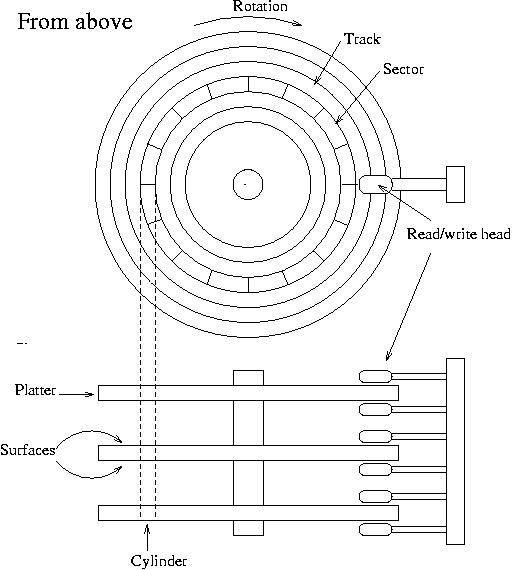
\includegraphics[height=0.8\textheight]{../../slides/disk/04-hd-schematic.png}
		\column{0.4\textwidth}
		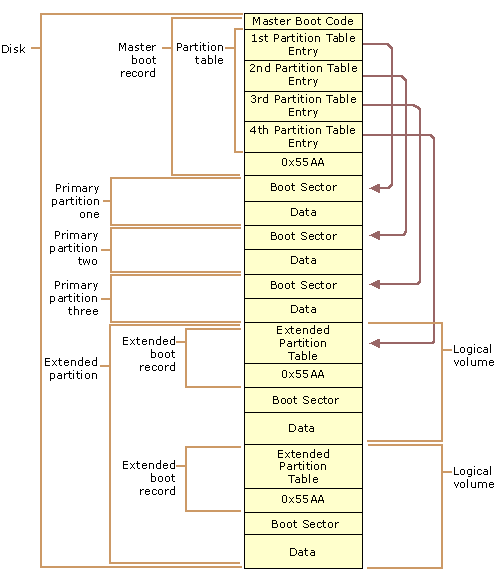
\includegraphics[height=0.8\textheight]{../../slides/disk/04-disk-structure.png}
	\end{columns}
\end{frame}

\begin{frame}{Отображение блочных устройств}


	\begin{block}{Device Mapper}
			{\tt /dev/mapper/*}\\
			device-mapper -- служит общим фреймворком для отображения одного блочного устройства на другое.

			Примеры: RAID, LVM, шифрованные диски и т.д.
	\end{block}

\end{frame}



}
\section{Основные команды}
\mode<all>{\begin{frame}{Полезные утилиты}
	\begin{columns}
		\column{0.25\textwidth}
		\begin{itemize}
			\item {\tt fdisk}
			\item {\tt parted}
			\item {\tt kpartx}
		\end{itemize}
		\column{0.25\textwidth}
		\begin{itemize}
			\item {\tt dd}
			\item {\tt losetup}
		\end{itemize}
		\column{0.25\textwidth}
		\begin{itemize}
			\item {\tt mkfs}
			\item {\tt fsck}
		\end{itemize}
		\column{0.25\textwidth}
		\begin{itemize}
			\item {\tt mount}
			\item {\tt umount}
			\item {\tt df}
		\end{itemize}
	\end{columns}

%	\bigskip
%	Понадобятся для упражнений:
%	\begin{itemize}
%			\item[*] {\tt chroot}
%			\item[*] {\tt kvm}
%	\end{itemize}
\end{frame}


\begin{frame}{Практика: отображение файла на loop-устройство}
	\begin{enumerate}
		\item Создать пустой файл размером 100MB: \\
			dd if=/dev/zero of=test bs=1M count=100
			\pause
		\item Найти неиспользуемое loop-устройство и отобразить на него файл:\\
			losetup -f \\
			losetup loop0 test
			\pause
		\item Посмотреть структуру loop-устройства, создать разделы и посмотреть результаты:\\
			fdisk -l /dev/loop0 \\
			fdisk /dev/loop0 \\
			fdisk -l /dev/loop0
			\pause
		\item Дать команду ядру перечитать разделы и создать устройства для разделов:\\
			ls -l /dev/mapper/* \\
			kpartx -a /dev/loop0 \\
			ls -l /dev/mapper/* \\
	\end{enumerate}
\end{frame}

\begin{frame}{Практика: создание файловой системы}
	\begin{enumerate}
		\item Форматируем файловую систему на устройстве: \\
			mkfs.ext2 /dev/mapper/loop0p1
			\pause
		\item и монтируем:\\
			mkdir -p /mnt/fs\\
			mount\\
			mount /dev/mapper/loop0p1 /mnt/fs\\
			mount\\
			df
			\pause
	\end{enumerate}
\end{frame}


\begin{frame}{Практика: чистимся}
	\begin{enumerate}
		\item Найти смонтированные разделы и отмонтировать их: \\
			mount \\
			umount /dev/mapper/loop0p1
			\pause
		\item Найти используемые loop-устройства\\
			losetup -a \\
			\pause
		\item Корректно удалить устройства для разделов:\\
			ls -l /dev/mapper/* \\
			kpartx -d /dev/loop0 \\
			ls -l /dev/mapper/* \\
			\pause
		\item Удалить отображение файла на loop-устройство: \\
			losetup -d /dev/loop0
	\end{enumerate}
\end{frame}


}
\section{GPT}
\mode<all>{\begin{frame}{GUID таблица разделов}

   \begin{columns}
      \column{0.5\textwidth}
      \begin{itemize}
        \item{Не менее 128 доступных разделов}
        \item{Дополнительные копии таблицы разделов}
        \item{$>1024^3$TB размер раздела}
        \item{Часть спецификации UEFI}
      \end{itemize}
      \column{0.5\textwidth}
      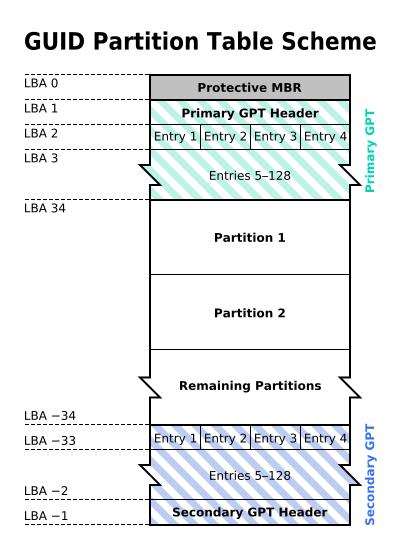
\includegraphics[width=0.9\textwidth]{../../slides/disk/gpt.png}
  \end{columns}
\end{frame}
\begin{frame}{Утилиты}
  \begin{itemize}
    \item gdisk (аналог fdisk)
    \item cgdisk (аналог cfdisk)
    \item parted
  \end{itemize}
\end{frame}

\begin{frame}{Источники по UEFI boot}
  \begin{itemize}
    \item http://www.rodsbooks.com/efi-bootloaders/
    \item http://www.slideshare.net/mlug/arch-onmac 
  \end{itemize}
\end{frame}
}
\section{LVM}
\mode<all>{\begin{frame}{LVM -- управление логическими томами}
  \begin{center}
    \textbf{Структура LVM}
  \end{center}
  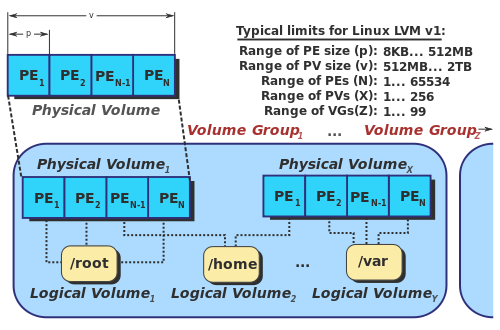
\includegraphics[width=0.7\textwidth]{../../slides/disk/LVM1-wiki.png}
\end{frame}

\begin{frame}{Преимущества LVM}
	\begin{itemize}
		\item Изменение размера
		\item Перемещение данных в активной системе
		\item Присвоение имен устройствам
		\item Чередование дисков
		\item Зеркалирование томов
		\item Снимки томов
	\end{itemize}
\end{frame}
 
\begin{frame}{LVM -- основные команды}
  \begin{itemize}
    \item Создание
      \begin{columns}
        \column{0.2\textwidth}
        \begin{itemize}
          \item pvcreate
        \end{itemize}
        \column{0.2\textwidth}
        \begin{itemize}
          \item vgcreate
        \end{itemize}
        \column{0.2\textwidth}
        \begin{itemize}
          \item lvcreate
        \end{itemize}
      \end{columns}
     \item Информация 
       \begin{columns}
         \column{0.2\textwidth}
         \begin{itemize}
           \item pvscan
           \item lvscan
           \item vgscan
		   \item lvmdiskscan
         \end{itemize}
         \column{0.2\textwidth}
         \begin{itemize}
           \item pvdisplay
           \item lvdisplay
           \item vgdisplay
		   \item[ ]
         \end{itemize}
         \column{0.2\textwidth}
         \begin{itemize}
           \item pvs
           \item lvs
           \item vgs
		   \item[ ]
         \end{itemize}
	 \end{columns}
      \item Манипулирование
        \begin{itemize}
          \item vgextend/vgreduce
          \item lvresize
          \item pvmove
          \item pvremove
         \end{itemize}
     \end{itemize}
    
\end{frame}

\begin{frame}{Упражнение: создание}
  \begin{enumerate}
    \item Создать 3 файла (200MB) и отобразить на {\tt /dev/loop[0-]}
	\item Найти устройства для работы с LVM {\tt lvmdiskscan}
	\item  {\tt pvcreate /dev/loop[0-2]}
    \item  {\tt pvscan, pvdisplay, pvs}
		\pause
    \item Создание группы томов {\tt vgcreate VG0 /dev/loop[0-2]}
    \item {\tt pvscan, vgscan, pvdisplay}
		\pause
    \item Создание логического тома {\tt lvcreate  -l 50\%VG -i 3 -n lv1 VG0}
	\item Создание файловой системы ext2 на {\tt /dev/VG0/lv1} и монтирование в {\tt /mnt/myfs}
	\end{enumerate}
\end{frame}


\begin{frame}{Упражнение: Создание снимка LVM}
  \begin{enumerate}
    \item Скопировать несколько файлов на { \tt /mnt/myfs}
    \item  {\tt lvcreate -\phantom{}-snapshot -l 10\%VG -n snap /dev/VG0/lv1}
    \item  {\tt lvdisplay, lvs, lvscan}
	\item Смонтировать снимок в {\tt /mnt/snap}
		\pause
    \item Удалить один из файлов на {\tt /mnt/snap/} или {\tt /mnt/myfs/}
	\item Отмонтировать снимок и оригинал
		\pause
	\item Объединяем снимок с оригиналом {\tt lvconvert -\phantom{}-merge VG0/snap}
	\item Монтируем {\tt /dev/VG0/lv1} в {\tt /mnt/myfs} и проверяем изменения
  \end{enumerate}
\end{frame}

\begin{frame}{Упражнение: изменение размера VG}
  \begin{enumerate}
%	\item Отмонтировать {\tt /mnt/myfs}
	\item Создать еще один файл и отобразить его на {\tt loop3}
	\item Увеличиваем размер группы {\tt vgextend VG0 /dev/loop3}
		\pause
    \item  {\tt pvscan; pvmove /dev/loop0; pvscan}
    \item  {\tt vgreduce VG0 /dev/loop0; pvscan}
    \item  {\tt pvremove /dev/loop0; pvscan}
  \end{enumerate}
\end{frame}


}

\chapter{Сетевая подсистема}

\section{Основы работы с сетевой подсистемой}

\mode<all>{\begin{frame}{Сетевая подсистема Linux}

	\begin{block}{Cетевой интерфейс}

		Сетевой интерфейс в Linux -– это абстрактный именованный объект,  используемый для передачи 
		данных через некоторую линию связи без привязки к ее (линии связи) реализации.
	\end{block}
\end{frame}

\begin{frame}{Сетевая подсистема Linux}

	\center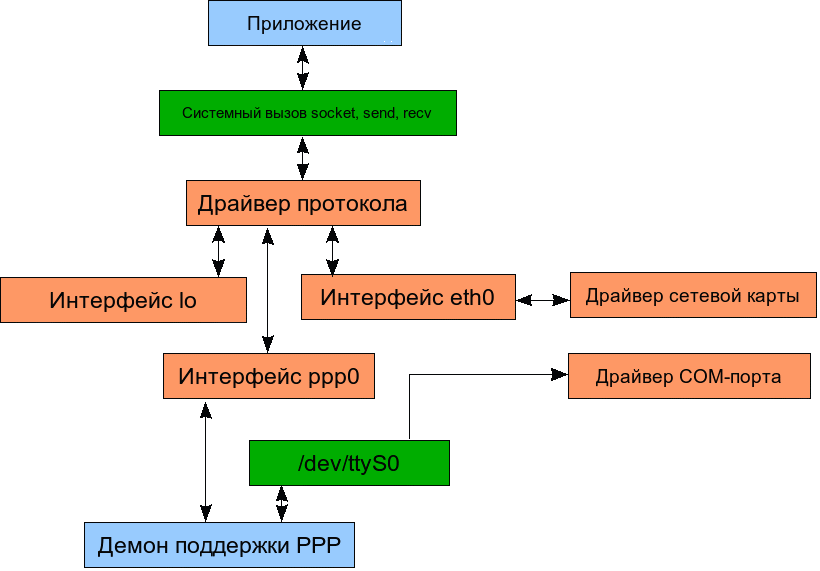
\includegraphics[height=0.8\textheight]{../../slides/networking/06-netstack.png}

\end{frame}


}

\subsection{Управление интерфейсами}
\mode<all>{\begin{frame}{Команды управления настройками сети}
	\begin{itemize}
	  \item ifconfig/route
	  \item iproute2
	\end{itemize}

	\begin{itemize}
		\item Список интерфейсов
			\begin{itemize}
				\item {\tt ifconfig -a}
				\item {\tt ip link show}
			\end{itemize}
		\item Включение интерфейса 
			\begin{itemize}
				\item {\tt ifconfig <iface> up}
				\item {\tt ip link set <iface> up}
			\end{itemize}
	  \item Выключение интерфейса
			\begin{itemize}
				\item {\tt ifconfig <iface> down}
				\item {\tt ip link set <iface> down}
			\end{itemize}
	  \item Назначение адреса
			\begin{itemize}
				\item {\tt ifconfig eth0 192.168.1.17 netmask 255.255.254.0 up}
				\item {\tt ip addr add 192.168.1.17/23 dev eth0}
			\end{itemize}
	\end{itemize}
\end{frame}

\begin{frame}{Конфигурационные файлы}
  \begin{itemize}
    \item {\tt /etc/resolv.conf}
    \item {\tt /etc/hosts}
	\item {\tt /etc/sysconfig/network}
    \item Расположение зависит от дистрибутива:
		\begin{itemize}
			\item RH-like: {\tt /etc/sysconfig/network-scripts}\\
				{\tt /etc/sysconfig/network-scripts/ifcfg-eth0}
			\item ALTLinux: {\tt /etc/net/ifaces}
			\item Debian: {\tt /etc/network/interfaces}
			\item Gentoo: {\tt /etc/conf.d/net}
		\end{itemize}
  \end{itemize}
\end{frame}

\begin{frame}{Дополнительные интерфейсы}
	\begin{block}{Алиасы}
		\begin{itemize}
			\item ifconfig <iface>:<alias> <ip> up
			\item ifconfig <iface> add <ip> up
			\item ip addr add <ip> {\bf label} <iface>:<alias> dev <iface>
		\end{itemize}
	\end{block}
	\pause
	\begin{block}{VLAN}
		\begin{itemize}
			\item vconfig add <iface> <id>
			\item vconfig rem <iface>{\bf.}<id>
			\item ip link add {\bf link} <iface> name <vlan\_name> {\bf type vlan id <id>}
			\item ip link delete <vlan\_name>
		\end{itemize}
	\end{block}

\end{frame}


}

\subsection{Полезные программы}
\mode<all>{\begin{frame}{Полезные утилиты}
	\begin{center}
		\begin{itemize}
			\item netstat / ss
			\item nslookup / dig
			\item ping
			\item traceroute
			\item tcpdump
			\item telnet
			\item netcat
			\item nmap
		\end{itemize}
	\end{center}

\end{frame}


\begin{frame}[allowframebreaks]{Полезные утилиты: практика}

		\begin{block}{netstat}

			Узнать:
			\begin{itemize}
				\item список используемых сокетов
				\item серверных сокетов
				\item имена/pid серверов
				\item узнать номера портов
			\end{itemize}
		\end{block}
	
		\framebreak
		\begin{block}{telnet/netcat}

			\begin{itemize}
				\item Чат по протоколу TCP с соседом
				\item Чат по протоколу UDP с соседом
				\item Передать текстовый и бинарный файлы
			\end{itemize}
	
			При создании чата использовать {\tt netstat} и {\tt tcpdump}
			для получения информации о соединении.
		\end{block}

		\framebreak
		\begin{block}{nmap}
			\begin{itemize}
				\item сканирование соседа
				\item сканирование выделенных портов у соседа (поиск сервера чата) 
				\item узнать список открытых портов на всех машинах в аудитории
				\item узнать список работающих машин
			\end{itemize}
		\end{block}
	
\end{frame}

tcpdump
0. pcap файлы/libpcap
1. запуск монитора
2. запуск чата
3. монитор-фильтр-анализ

}

\section{ssh}
\mode<all>{\begin{frame}{ssh}

	\begin{block}{ssh -- терминал}
		{\tt ssh [user@]host[:port]}\\
		{\tt ssh host [-l user] [-p port]}
		\begin{itemize}
			\item -v -- "разговорчивый" режим 
			\item -t -- насильное назначение псевдотерминала (для автоматизации)
		\end{itemize}
		Вся конфигурация пользователя: {\tt \$HOME/.ssh}
	\end{block}

	\pause

	\begin{block}{... и не только}
		\begin{itemize}
			\item -X -- "проброс" графики 
			\item -L [bindip:]port:rhost:rport -- "пробрасывание" порта с удаленной машины на локальную
			\item -R [bindip:]port:lhost:lport -- "пробрасывание" порта с локальной машины на удаленную
			\item -W host:port -- stdin/stdout с указанным хостом
			\item -D port -- динамический прокси
		\end{itemize}
	\end{block}
\end{frame}


}


\section{Дополнительные типы интерфейсов}

\subsection{alias, vlan}
\mode<all>{
\begin{frame}{Дополнительные интерфейсы}
	\begin{block}{Алиасы}
		\begin{itemize}
			\item ifconfig <iface>:<alias> <ip> up
			\item ifconfig <iface> add <ip> up
			\item ip addr add <ip> {\bf label} <iface>:<alias> dev <iface>
		\end{itemize}
	\end{block}
	\pause
	\begin{block}{VLAN}
		\begin{itemize}
			\item vconfig add <iface> <id>
			\item vconfig rem <iface>{\bf.}<id>
			\item ip link add {\bf link} <iface> name <vlan\_name> {\bf type vlan id <id>}
			\item ip link delete <vlan\_name>
		\end{itemize}
	\end{block}

\end{frame}


}
\subsection{Мосты}
\mode<all>{\begin{frame}{Мосты}
	\begin{itemize}
		\item Создать -- {\tt brctl addbr <bridge>}
		\item Удалить -- {\tt brctl delbr <bridge>}
		\item Добавить интерфейс -- {\tt brctl addif <bridge> <device>}
		\item Удалить интерфейс-- {\tt brctl addif <bridge> <device>}
	\end{itemize}
\end{frame}


}
\subsection{Тоннели}
\mode<all>{
\begin{frame}{''Виртуальные'' интерфейсы}
	\begin{block}{TUN/TAP}

		{\tt modprobe tun}

		\begin{itemize}
			\item Добавить интерфейс TUN -- {\tt tunctl -n -t <ifacename>}
			\item Добавить интерфейс TAP -- {\tt tunctl -p -t <ifacename>}
			\item Удалить интерфейс -- {\tt tunctl -d <ifacename>}
		\end{itemize}
	\end{block}

	\pause

	\begin{block}{Практика}
		\begin{itemize}
			\item Создать интерфейс TAP с именем {\tt mytap}
			\item Создать мост с именем {\tt mybr}
			\item Назначить интерфейсу {\tt mytap} адрес {\tt 192.168.0.<n>/24}
			\item Добавить интерфейсы {\tt mytap} и {\tt eth0} к мосту {\tt mybr}
			\item Запустить {\tt tcpdump} на интерфейсах {\tt mybr} и {\tt mytap}
			\item Запустить {\tt ping} соседа
		\end{itemize}
	\end{block}

\end{frame}


}

\section{Маршрутизация}
\mode<all>{\begin{frame}{Маршрутизация}
	\begin{itemize}
		\item netstat -r
		\item route
		\item ip route show
	\end{itemize}

	\begin{block}{Разрешить маршрутизацию на хосте}
		{\tt echo 1 > /proc/sys/net/ipv4/ip\_forward}
	\end{block}
\end{frame}


}

\section{iptables}
\mode<all>{\begin{frame}{Iptables}

	\center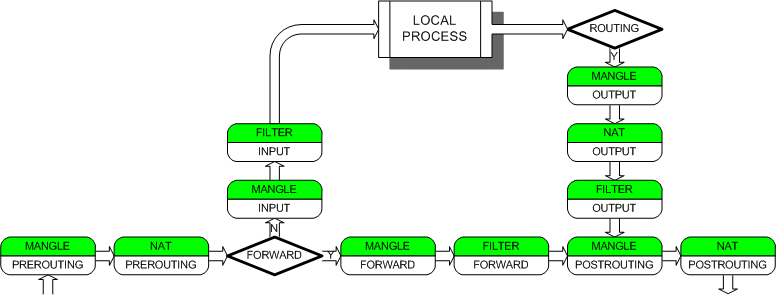
\includegraphics[height=0.4\textheight]{../../slides/networking/06-iptables.png}

	\begin{itemize}
	\begin{columns}
		\column{0.3\textwidth}
			\item[ ] {\bf iptables -L -t <table>}
				\bigskip

			\item filter -- файерволл
				\begin{itemize}
					\item INPUT
					\item FORWARD
					\item OUTPUT
				\end{itemize}
		\column{0.3\textwidth}
			\item nat -- преобразования адресов
				\begin{itemize}
					\item PREROUTING
					\item INPUT
					\item OUTPUT
					\item POSTROUTING
				\end{itemize}
		\column{0.3\textwidth}
			\item mangle -- специальные  изменения  пакетов (TOS, TTL, MARK)
				\begin{itemize}
					\item PREROUTING
					\item INPUT
					\item FORWARD
					\item OUTPUT
					\item POSTROUTING
				\end{itemize}
		\end{columns}
	\end{itemize}

\end{frame}


}

\chapter{Самостоятельная работа}
\mode<all>{\begin{frame}{Практика: создание тестовой среды}

	\center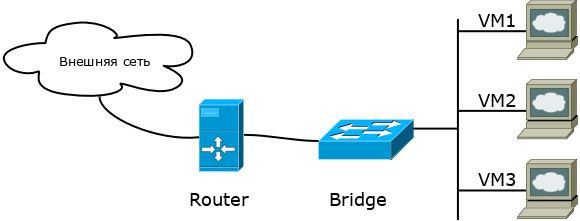
\includegraphics[height=0.4\textheight]{../../slides/networking/net-practice.png}


	\begin{block}{Задача}
		Запустить 3 идентичные виртуальные машины.\\
		Каждой машине назначить адрес из отдельного IP диапазона.\\
		Организовать сетевую ''видимость'' между виртуальными машинами, а также хостом.		
	\end{block}

\end{frame}



\begin{frame}
	\frametitle{Подготовка дисковой подсистемы}
			\begin{itemize}
				\item Создать пустой файл размером в 1.5 GB и отобразить на устройство
					/dev/loop ({\tt dd, losetup})
				\item Создать группу томов на базе этого устройства ({\tt pvcreate, vgcreate})
				\item Выделить 1 GB под логический диск ({\tt lvcreate})
				%\item Скопировать образ виртуального диска в полученный логический том ({\tt dd})
				%\item Создать снимок логического тома на 100MB ({\tt lvcreate}) для каждой виртуальной машины.
			\end{itemize}
\end{frame}

\begin{frame}[fragile]{Установка системы}
        \begin{itemize}
			\item Установить centos-minimal на  машину из iso файла.
            \item Создать два снимка логического тома виртуальной машины
			\item Убедиться в наличии tap интерфейсов
		\end{itemize}

\end{frame}

\begin{frame}[fragile]{Пример запуска kvm}
		\begin{itemize}
          \item {\tt modprobe kvm-intel} {\small Включаем модуль поддержки виртуализации в ядре} 
          \item {\tt modprobe tun}  {\small Включаем поддержку tun, tap виртуальных сетевых интерфейсов}
          \item 
            \begin{lstlisting}[language=bash,basicstyle=\tiny] 
kvm -enable-kvm -cdrom centos-minimal.iso -hda /dev/loop0 -m 512M   \
    -boot order=cd -serial stdio -net nic,model=rtl8139 -net tap,ifname=tap0 
            \end{lstlisting}
              \begin{enumerate}
                \item[{\tt -enable-kvm}] Включает ядерную поддержку виртуализации
                \item[{\tt -cdrom}] Устройство или disk image, cdrom виртуальной машины
                \item[{\tt -hda}] Устройство или disk image, представляет жесткий диск VM
                \item[{\tt -serial}] Перенаправление com порта (консоль ядра)
                \item[{\tt -net nic}] Условная модель сетевой карточки
                \item[{\tt -net tap}] TAP интерфейс, на который будет приходить сеть из VM
                \item[{\tt -boot order}] cd (вначале cdrom (с), потом диск (d))
                \item[{\tt -m}] Объем памяти для VM
              \end{enumerate}
        \end{itemize}
\end{frame}        


\begin{frame}
	\frametitle{Настройка сети на хосте}
			\begin{itemize}
				\item Создать мост {\tt brctl} и назначить ему адреса из соответствующих диапазонов {\tt ifconfig/ip}
				\item Поднять виртуальные интерфейсы {\tt ifconfig/ip}
				\item Добавить виртуальные интерфейсы к мосту {\tt brctl}
			\end{itemize}
\end{frame}


\begin{frame}
	\frametitle{Настройка сети на виртуальных машинах}
			\begin{itemize}
				\item Назначить адрес устройству eth0 {\tt ifconfig/ip}
				\item Добавить адрес маршрутизатора по умолчанию {\tt route/ip}
				\item Проверить доступность виртуальных машин и хоста {\tt ping/nmap}
			\end{itemize}
\end{frame}

\begin{frame}
	\frametitle{Настройка роутинга и NAT}
			\begin{itemize}
				\item Разрешить форвардинг на хосте
				\item Настроить NAT на хосте ({\tt iptables},  правило {\tt MASQUERADE})
				\item Проверить доступность хостов из ''внешней'' сети {\tt ping/nmap}
			\end{itemize}
\end{frame}


}
}


\part{BASH}
\chapter*{Bourne Again Shell}
\section{Переменные}
\mode<all>{%% Vars


\begin{frame}
	\frametitle{Переменные} 
	\large\center{Нетипизированные!!!}

	Для прямого обращения необходимо использовать префикс \\
	\center{\Large{\tt \$}}

	Фигурные скобки используют для отделения от текста:\\
	\center{\tt \$VARrest != \$\{VAR\}rest}

	%\bigskip
	
	\begin{alertblock}{Используют без префикса}
		\begin{itemize}
			\item В объявлении declare или присвоении
			\item в командe {\tt read}
			\item unset -- удаление
			\item В арифметических операциях {\tt (( ... ))}
		\end{itemize}
	\end{alertblock}
\end{frame}

\begin{frame}[fragile]
	\frametitle{Задание. Присвоить переменной значение.}

	\begin{lstlisting}
#!/bin/bash

VAR=string
echo $VAR
	\end{lstlisting}


	\begin{block}{Изменить и посмотреть на результат.}
		\begin{itemize}
			\item Добавить пробел до знака ''{\tt =}''
			\item Добавить пробел после знака ''{\tt =}''
			\item Присвоить переменной VAR значение: I love \$\$\$!
			\item Создать переменные с другим именем и значением var 1var \_var var1
		\end{itemize}
	\end{block}

\end{frame}

\begin{frame}[fragile]
	\frametitle{Косвенное обращение к переменной}

	Косвенное (indirect) обращение к переменной: {\tt \$\{!VARIABLE\}}

	\begin{block}{Пример}
		\begin{lstlisting}
#!/bin/bash 
num=$# 
lastarg=${!num} 
echo $num $lastarg
		\end{lstlisting}
	\end{block}

\end{frame}


\begin{frame}
	\frametitle{Типы переменных}
	\begin{itemize}
		\item Локальные\\
		    Область видимости -- текущая программа, функция или субшелл
		\item Окружения
		\item Позиционные параметры
	\end{itemize}
\end{frame}



\begin{frame}
	\frametitle{Внешние переменные}

	\center{Наследование внешней переменной}

	\begin{itemize}
		\item export
		\item Переданное в командной строке \\
			\begin{block}{Пример}
				{\tt TEST=123 make}
			\end{block}
	\end{itemize}
\end{frame}


\begin{frame}[fragile]
	\frametitle{Специальные переменные}

	Часто используемые в скриптах:

	\begin{itemize}
		\item Разделитель \$IFS
		\item Директории -- домашняя \$HOME и текущая \$PWD
		\item UID пользователя -- \$UID
		\item ID процесса -- \$\$
		\item Имя хоста -- \$HOSTNAME
		\item Вид командной строки: \$PS1 -- \$PS4
		\item Локализация
			\begin{itemize}
				\item Используемый язык \$LANG
				\item Локализация \$LC\_ALL
					\begin{block}{Пример}
						\begin{lstlisting}
ls -l 
LC_ALL=C ls -l
						\end{lstlisting}
					\end{block}
			\end{itemize}
	\end{itemize}

\end{frame}



}
\section{Скрипты и запуск}
\mode<all>{

\begin{frame}[fragile]
	\frametitle{Введение}

	\begin{block}{Sha-Bang}
		\begin{lstlisting}
#!/bin/bash
		\end{lstlisting}
	\end{block}

	\begin{block}{Режим совместимости с POSIX}
		\begin{lstlisting}
#!/bin/sh
		\end{lstlisting}

	\end{block}

\end{frame}


\begin{frame}
	\frametitle{Спецсимволы}

	\begin{itemize}
		\item \# -- Вся строка после \# является комментарием
		\item ; -- Разделение команд
		\item : -- NOP оператор (похож на встроенный вызов true)
		\item {\tt source} или {\bf .} -- скрипт выполняется в текущем экземпляре shell
	\end{itemize}

\end{frame}


\begin{frame}
	\frametitle{Спецсимволы}

	\begin{block}{Фигурные скобки и склеивание с помощью ``,``}
		\begin{itemize}
			\item Посмотреть на результат выполнения команды \\
				{\tt echo \{A,B,C\}:\{1,2,3\}}
				\pause
			\item Посмотреть на результат выполнения команды \\
				{\tt ls -l \{,/usr\}/\{bin,sbin\}/*sh}
		\end{itemize}
	\end{block}

\end{frame}


\begin{frame}[fragile]
	\frametitle{Экранирование}

	\begin{columns}
		\column{0.5\textwidth}
		\begin{itemize}
			\item Экранирование одного символа \textbackslash 
			\item Частичное экранирование ''
			\item Полное экранирование '
		\end{itemize}
		\pause
		\column{0.5\textwidth}
		Спецзначения для echo и sed
		\begin{itemize}
			\item \textbackslash{n} -- новая строка
			\item \textbackslash{r} -- возврат каретки
			\item \textbackslash{t} -- табуляция
			\item \textbackslash{v} -- вертикальная табуляция \\
				\small\begin{lstlisting}
echo -e "test \v test \v test"
				\end{lstlisting}
			\item \textbackslash{b} -- перемещение на 1 символ назад
			\item \textbackslash{a} -- звуковой сигнал
			\item \textbackslash{0xxx} -- 8-миричное число
			\item \textbackslash{xXXX} -- 16-ричное число
		\end{itemize}
	\end{columns}

\end{frame}


\begin{frame}
	\frametitle{Подстановка команд}
	
	Синтаксис:

	\begin{itemize}
		\item \`{}command\`{}
		\item \$(command)
	\end{itemize}
	\pause
	\begin{block}{Задание}
		Присвоить переменной LIST результат выполнения команды {\tt ls -1} \\
		Вывести на экран переменную LIST
	\end{block}
\end{frame}

\begin{frame}[fragile]
	\frametitle{Коды возврата}

	Согласно POSIX: 0 -- успех

	Код возврата доступен через переменную \$?

	\pause
	\begin{block}{Пример}
		\begin{lstlisting}
/bin/true; echo $?
/bin/false; echo $?
		\end{lstlisting}
	\end{block}

	Скрипт возвращает код последней команды, поэтому для корректного выхода необходимо использовать {\tt exit}.

\end{frame}


\begin{frame}
	\frametitle{exec}

	Заменяет текущий shell переданной командой. 

	Часто используется для переназначения файловых дескрипторов.

\end{frame}

\begin{frame}
	\frametitle{Управление заданиями}
	
	\begin{itemize}
		\item {\tt bg} -- поместить задачу в фоновое исполнение
		\item {\tt fg} -- ''переключиться'' на задачу
		\item {\tt jobs} -- список активных задач
		\item {\tt wait [pid|id]} -- ждать завершения всех, либо конкретных задач
	\end{itemize}
	\pause
	\begin{block}{Задание}
		\begin{itemize}
			\item Запустить задачу ''{\tt sleep 100 \&}'' в фоновом режиме
			\item Запустить задачу ''{\tt sleep 100}'' на текущей косоли и остановить ее (Ctrl-Z)
			\item С помощью команды ''{\tt jobs}'' посмотреть статус активных задач
			\item С помощью команды ''{\tt bg}'' перевести остановленную задачу в фоновый режим
			\item С помощью команды ''{\tt fg}'' переключиться на одну из фоновых задач
		\end{itemize}
	\end{block}
\end{frame}



\begin{frame}[fragile]
	\frametitle{Группировка}
	
	\begin{block}{Пример}
		\begin{lstlisting}
( echo 1; echo 2) | tee file
		\end{lstlisting}
	\end{block}

	\pause
	\begin{block}{( cmd1; cmd2)}
	    Запускается новый shell
	\end{block}

	\begin{block}{Пример}
		\begin{lstlisting}
TEST=42; (echo $TEST; TEST=0; echo $TEST ); echo $TEST
		\end{lstlisting}
	\end{block}

\end{frame}


\begin{frame}[fragile]
	\frametitle{Перенаправление ввода/вывода}

	\begin{itemize}
		\item ``>'' -- Перенаправление в файл
			\begin{block}{Пример}
				\begin{lstlisting}
echo stdout > test.txt
				\end{lstlisting}
			\end{block}
		\item ``>\&'' -- Перенаправление в другой дескриптор
			\begin{block}{Пример}
				\begin{lstlisting}
(echo stdout; echo stderr >&2) > test.txt
				\end{lstlisting}
			\end{block}
	\end{itemize}

\end{frame}



\begin{frame}[fragile]
	\frametitle{Перенаправление ввода/вывода}

	\begin{itemize}

		\item ``\&>''
			\begin{block}{Пример}
				\begin{lstlisting}
(echo stdout; echo stderr >&2) &> test.txt
				\end{lstlisting}
			\end{block}
		
		\item ``>>'' -- Добавление в файл
			\begin{block}{Пример}
				\begin{lstlisting}
echo stdout >> test.txt
				\end{lstlisting}
			\end{block}
																										                
		\item ``<'' -- Чтение из файла
			\begin{block}{Пример}
				\begin{lstlisting}
cat < test.txt
				\end{lstlisting}
			\end{block}
	\end{itemize}

\end{frame}


\begin{frame}[fragile]
	\frametitle{Перенаправление ввода/вывода}

	\begin{itemize}

		\item ``<<'' -- Here-документ

		\item ``<>'' -- Открывает файловый дескриптор из файла/другого дескритора
			\begin{block}{Пример}
				\begin{lstlisting}
exec 3<>test.txt; echo test >&3;  cat <test.txt
				\end{lstlisting}
			\end{block}
			
		\item ``n<\&-'' -- Закрывает файловый дескриптор
			\begin{block}{Пример}
				\begin{lstlisting}
exec 3<&-; echo test >&3
				\end{lstlisting}
			\end{block}
			
		\item ``|'' -- pipe
	\end{itemize}

\end{frame}


}
\section{Параметры}
\mode<all>{
\begin{frame}
	\frametitle{Позиционные параметры}

	\begin{itemize}
		\item \$0-9 -- значение соответствующего параметра
		\item \$\# -- еоличество переданных параметров
		\item \$* -- представляется, как одна строка
		\item \$@ -- каждый параметр, как отдельная строка
	\end{itemize}

\end{frame}


\begin{frame}[fragile]
	\frametitle{shift}

	Встроенная команда сдвига параметров влево.

	В качестве параметра может принимать число -- на сколько параметров сдвигать.

	\begin{lstlisting}
shift [num]
	\end{lstlisting}

\end{frame}


\begin{frame}
	\frametitle{Задание}

	\begin{enumerate}
		\item Написать скрипт,  который выдает количество переданных параметров
			\pause
		\item Вывести на экран имя команды
			\pause
		\item Сделать symlink на скрипт и запустить
			\pause
		\item Вывести на экран первых 3 параметра
			\pause
		\item Передать строку "I am user \$USER" в качестве параметра
			\begin{itemize}
				\item Без экранирования
				\item С экранированием ''
				\item С экранированием '
			\end{itemize}
			\pause
		\item Добавить shift перед выводом параметров
	\end{enumerate}
\end{frame}


}
\section{Тесты и сравнения}
\mode<all>{%%

\begin{frame}{Общий синтаксис}

	Условие:
	\begin{itemize}
		\item Exit status любой программы
		\item test или $[$ 
		\item Двойные скобки {\bf (( ... ))} и конструкция {\bf let}
	\end{itemize}


	Конструкция для сравнения:
	\begin{itemize}
		\item \&\& и ||
		\item if/then/else
	\end{itemize}

\end{frame}

\begin{frame}[fragile]{Двойные скобки и {\bf let}}

	Позволяют производить арифметические вычисления!

	\pause
	Пример:
\begin{lstlisting}[language=bash]
a=$(( 5 + 3 ))
let "b = (( a + 10 ))"
echo $a $b
\end{lstlisting}

	\pause
	Операции:
	\begin{itemize}
		\item (( 0 \&\& 1 )) -- логическое "И"
		\item (( 0 || 1 )) -- логическое "ИЛИ"
		\item (( 0 \& 1 )) -- побитовое "И"
		\item (( 0 | 1 )) -- побитовое "ИЛИ"
	\end{itemize}

	{\bf Практическое задание:} \\
	написать скрипт, которому в качестве параметров передается 2 значения. Вывести на экран результаты логических и побитовых операций. 
\end{frame}


\begin{frame}[fragile]{test}

	\begin{itemize}
	    \item ! -- отрицание
	    \item -z СТРОКА
	    \item СТРОКА1 = СТРОКА2
	    \item СТРОКА1 != СТРОКА2
	    \item ЦЕЛОЕ1 -eq ЦЕЛОЕ2
	    \item ЦЕЛОЕ1 -ge ЦЕЛОЕ2
	    \item ЦЕЛОЕ1 -lt ЦЕЛОЕ2
	    \item -d ФАЙЛ
	    \item -e ФАЙЛ
	    \item -f ФАЙЛ
	\end{itemize}

\end{frame}

\begin{frame}[fragile]{\&\& и ||}
	Синтаксис:
\begin{verbatim}
условие && true || false
\end{verbatim}

	\pause
	Пример:
\begin{lstlisting}[language=bash]
test -z "$DISPLAY" && echo "text mode" || echo "graphical mode"
\end{lstlisting}
	
	\pause

	\begin{itemize}
	    \item Запустить команды "true" и "false"
	    \item В случае успеха вывести "успех"
	    \item В случае неуспеха вывести "неудача"
	\end{itemize}
\end{frame}



\begin{frame}[fragile]{Синтаксис {\bf if}}

	\begin{columns}
		\column{0.4\textwidth}
	
	\begin{lstlisting}[language=bash]
if [ условие1 ]
then
   . . .
elif [ условие2 ]
then
   . . .
else
   . . .
fi
\end{lstlisting}
		\column{0.6\textwidth}
	{\bf Практическое задание:} \\
	\begin{itemize}

		\item с помощью конструкции {\bf if} проверить существует ли файловый объект передаваемый в качестве параметра скрипту
		\item если нет, то создать директорию с таким именем
		\item если cуществует и файл является shell-скриптом, то запустить его
		\item если существует и является директорией, то вывести на экран первых 5 файлов в этой директории
	\end{itemize}
	\end{columns}
\end{frame}


%\begin{frame}[fragile]{}

%\end{frame}

}
\section{Арифметические операции}
\mode<all>{%% Arithmetic

\begin{frame}
  \frametitle{}
  \begin{itemize}
   \item  Конструкция {\tt ((...))}
    \begin{block}{Примеры}
     {\tt (( a=10 )); echo \$(( a++ )); echo \$a; } 
    \end{block}
    \pause
   \item  {\tt let}
    \begin{block}{Примеры}
     {\tt let a=10; echo \$a; let a+=-2; echo \$a; echo \$(( $--$a)); echo \$a} 
    \end{block}
    \pause
   \item  {\tt expr } внешняя команда 
    \begin{block}{Пример}
       { \tt x=\`{}expr \$x + 1\`{} }
    \end{block}
  \end{itemize}
\end{frame}

\begin{frame}[fragile]
\frametitle{Операторы в арифметических выражениях}
\begin{enumerate}
\item Инкременты, декременты {\tt id++, id$--$, ++id, $--$id } 
\item Арифметические операторы {\tt **,*,/,\%,+,-} 
\item Побитовые операторы {\verb+ ~,>>,<<,^,&,|+}
\item Операторы сравнения {\tt <=,>=,<,>, ==, !=}
\item Логические операторы {\tt \&\&, || } 
\item Тернарный оператор {\tt expr ? expr : expr }
\item Операторы присваивания
\begin{lstlisting}[language=C]
=, *=, /=, %=,
+=, -=, <<=, >>=,
&=, ^=, |=  
\end{lstlisting}
\end{enumerate} 

  
\end{frame}


\begin{frame}[fragile]
  \frametitle{Упражнение}
 \begin{enumerate}
   \item {\bf Конец света:} Вывести дату конца юниксовых времен ( время $2^{31}-1$) {\tt date -d @<seconds> } 
   \item Проверить результат арифметической операции (( 5>10 ))
 \end{enumerate}
\end{frame}
}
\section{Циклы}
\mode<all>{\begin{frame}
\frametitle{Основные конструкции для циклов}
  \begin{itemize}
   \item while
   \item for
   \item until
   \item break, continue 
   \item внешние команды find, xargs 
  \end{itemize}
\end{frame}

\begin{frame}[fragile]
  \frametitle{Циклы for}
  \begin{enumerate}
    \item Стандартная форма
\begin{lstlisting}[language=sh,frame=single]
  for x in list 
  do
    op1
    op2
  done
\end{lstlisting}
    \item Арифметическая форма
\begin{lstlisting}[language=sh,frame=single]
  for (( expr1 ; expr2 ; expr3 )) 
  do 
    op1
    op2
  done
\end{lstlisting}
  \end{enumerate}
\end{frame}

\begin{frame}[fragile]
\frametitle{ Циклы for. Примеры.}
  \begin{block}{Действие над файлами.}
\begin{lstlisting}[language=sh,frame=single]
for file in *
 do md5sum $file
done
\end{lstlisting}
  \end{block}

\begin{block}{Перечисление элементов.}
\begin{lstlisting}[language=sh,frame=single]
for planet in Mars Earth Mercury Saturn
 do echo $planet 
done
\end{lstlisting}
  \end{block}
\end{frame}

\begin{frame}[fragile]
\frametitle{ Циклы for. Примеры.}
  \begin{block}{Перечисление цифровой последовательности.}
\begin{lstlisting}[language=sh,frame=single]
for num in 1 2 3 4 5 6 7 8 9 10
 do echo $num
done

for num in $(seq 1 10)  # генерация из внешней команды
 do echo $num
done

for num in {1..10}  # генерация встроенными средствами
 do echo $num
done

\end{lstlisting}
  \end{block}
\end{frame}

\begin{frame}[fragile]
\frametitle{ Циклы for. Примеры.}
  \begin{block}{Перечисление цифровой последовательности C-like }
\begin{lstlisting}[language=sh,frame=single]
for ((i=1;i<11;i++))
do 
  echo $i
done  
\end{lstlisting}
  \end{block}

  \begin{block}{Несколько переменных}
    \begin{lstlisting}[language=sh,frame=single]
for ((a=1, b=1; a <= LIMIT ; a++, b++))
do
  echo -n "$a-$b"
done
    \end{lstlisting}
  \end{block}
\end{frame}

\begin{frame}[fragile]
\frametitle{ Циклы for. Примеры.}
  \begin{block}{Пустые выражения. Результат по умолчанию 1. }
    \begin{lstlisting}[language=sh,frame=single]
for (( i=1; ; i++))
do
  echo $i 
  [ "$i" -eq 10 ] && break 
done
    \end{lstlisting}
  \end{block}
\end{frame}

\begin{frame}[fragile]
\frametitle{ Циклы for. Примеры.}
  \begin{block}{Из аргументов.}
    \begin{lstlisting}[language=sh,frame=single]
for arg
 do echo $arg 
done
    \end{lstlisting}
  \end{block}
  \begin{block}{Из переменной. Запись одной строкой.}
    \begin{lstlisting}[language=sh,frame=single]
for name in $users ; do echo $name ; done
    \end{lstlisting}
  \end{block}
\end{frame}

\begin{frame}[fragile]
\frametitle{Циклы while,until}
\begin{lstlisting}[language=sh,frame=single]
while expr1; ... exprN
do
 op
done
\end{lstlisting}
\end{frame}

\begin{frame}[fragile]
\frametitle{}

\begin{block}{Пример. Перебираем аргументы.}
\begin{lstlisting}[language=sh,frame=single]
while [[ -n $1 ]]
do
    echo $1
    shift
done
\end{lstlisting}
\end{block}

\begin{block}{Пример. Несколько команд.}
\begin{lstlisting}[language=sh,frame=single]
while ((i++))
 read y
do
 echo $i $y
 [[ "$y" = 'stop' ]] && break
done
\end{lstlisting}
\end{block}
\begin{block}{Пример. Бесконечный цикл.}
\begin{lstlisting}[language=sh,frame=single]
while :
do
 x=$RANDOM
 echo $x
 [[ $x -gt 1100 ]] && break
done
\end{lstlisting}
\end{block}
\end{frame}

\begin{frame}[fragile]
\frametitle{ Цикл until. Пример.}
  \begin{block}{Ожидаем хост после перезагрузки.}
    \begin{lstlisting}[language=sh,frame=single]
until ping -q -c 3  $host 1>/dev/null 2>&1 && nc -z $host 22
do 
   sleep 1
   echo unavailable;
done
    \end{lstlisting}
  \end{block}
\end{frame}

\begin{frame}[fragile]
\frametitle{Перенаправление.}
Применяется ко всем командам внутри цикла.
  \begin{block}{Pipe}
    \begin{lstlisting}[language=sh,frame=single]
for name in $users ; do echo $name ; done | wc -l
    \end{lstlisting}
  \end{block}
  \begin{block}{В файл}
    \begin{lstlisting}[language=sh,frame=single]
for name in $users ; do echo $name ; done
(( i=10 )); while (( i > 0 )); do 
    echo "$i"
    (( i-- ))
done > output.txt
    \end{lstlisting}
  \end{block}
\end{frame}

\begin{frame}[fragile]
\frametitle{Внешние команды.}
Массовые операции с файлами.
  \begin{block}{Команда find}
    \begin{lstlisting}[language=sh,frame=single]
find . -name '*.c' -exec stat  {} \;
    \end{lstlisting}
  \end{block}
  \begin{block}{Команда xargs}
    \begin{lstlisting}[language=sh,frame=single]
echo /dev/std* | xargs -n1 readlink
    \end{lstlisting}
  \end{block}
\end{frame}

\begin{frame}[fragile]
    \frametitle{Упражнения}
    \begin{enumerate}
        \item Посчитать сумму кубов чисел от 1 до 100
        \item Вывести в файл 10 случайных чисел от 0 до 80
        \item Построить гистограмму данных из предыдущего файла файла {\bf Hint:} {\tt while read, echo -n }
    \end{enumerate}
\end{frame}
}
\section{Условные операторы}
\mode<all>{\begin{frame}[fragile]
\frametitle{Условные операторы: if}
\begin{itemize}
\item {\tt if;then;else;fi}
\begin{lstlisting}[language=sh,frame=single]
if CONDITIONS
then 
 OPS
[elif] CONDITIONS
[then]
 OPS
[else]
 OPS
fi
\end{lstlisting}
\end{itemize}
\end{frame}

\begin{frame}[fragile]
\frametitle{Условные операторы: case}
\begin{itemize}
\item {\tt case}
\begin{lstlisting}[language=sh,frame=single]
case "$variable" in 
 pattern1) command1
           command2
          ;;
 pattern2|pattern3)
         command3
         command4
        ;;
esac
\end{lstlisting}
\end{itemize}
\end{frame}

\begin{frame}[fragile]
\frametitle{Использование case вместе с getopts}
\begin{lstlisting}[language=sh,frame=single]
while getopts "af:h" Option
do
  case $Option in 
    a) OPTA=1 ;;
    f) OPTFILE=1
       FILENAME=$OPTARG
       ;;
    h) echo "Usage: $0 [-ah] -f <filename>";;
  esac  
done
shift $((OPTIND-1))
\end{lstlisting}
\end{frame}

\begin{frame}[fragile]
\frametitle{Упражнение}
\begin{enumerate}
\item Написать программу, которая по опции {\tt -h } выводит помощь, без опций выводит время в stdout,
с опцией -f выводит время в указаный файл
\end{enumerate}
\end{frame}
}
\section{Функции}
\mode<all>{\begin{frame}
	\frametitle{Функции}

	\begin{itemize}
		\item Именованные
		\item Неименованные
	\end{itemize}

	Функции в shell могут использоваться как обычные программы, которые:
	\begin{itemize}
		\item Принимают позиционные параметры;
		\item возвращают статус;
		\item Могут использоваться в качестве источника либо приемника 
			при перенаправлениях ввода/вывода.
	\end{itemize}

\end{frame}


\begin{frame}[fragile]
	\frametitle{Функции: синтаксис}
	\begin{itemize}
		\item Классический синаксис: 
			\begin{lstlisting}
function function_name {
command...
} 
			\end{lstlisting}
		\item Портабельный (C-style):
			\begin{lstlisting}
function_name()
{
command...
} 
			\end{lstlisting}

		\item Однострочный:
			\begin{lstlisting}
function_name () { command... ;}
			\end{lstlisting}
  \end{itemize}
\end{frame}

\begin{frame}[fragile]
	\frametitle{Пример (начало)}
	\small
	\begin{lstlisting}
#!/bin/bash

function help {
	echo "Использование: $0 <string>"
	exit 1
}
f1(){
	echo Вызвана функция $0 с $# аргументами
}

f2(){
	while read str; do
		echo $0 прочитана строка: $str
	done
}
	\end{lstlisting}

\end{frame}



\begin{frame}[fragile]
	\frametitle{Пример (окончание)}
	\small
	\begin{lstlisting}
[ $# -eq 0 ] && help

f1 "$@"

{ for ((i=0;i<5;i++));do
	echo $@
done } | f2

exit
	\end{lstlisting}

\end{frame}

\begin{frame}
	\frametitle{}
	\begin{itemize}
		\item 
		\item 
		\item
  \end{itemize}
\end{frame}

\begin{frame}
	\frametitle{}
	\begin{itemize}
		\item 
		\item 
		\item
  \end{itemize}
\end{frame}

\begin{frame}
	\frametitle{}
	\begin{itemize}
		\item 
		\item 
		\item
  \end{itemize}
\end{frame}

\begin{frame}
	\frametitle{}
	\begin{itemize}
		\item 
		\item 
		\item
  \end{itemize}
\end{frame}



}
\section{Массивы}
\mode<all>{\begin{frame}[fragile]
\frametitle{Основные операции с массивами}
\begin{itemize}
\item Присвоение значений
 \begin{itemize}
   \item \verb+ a=( "aaa" "bbb ccc" 2 ) +
   \item \verb+ a[1]="aaaa"; a[3]="bb bb";   +
   \item \verb+ a=( [1]="aaa" [10]="bbb"); +
 \end{itemize}
\item Доступ к значениям \verb+ echo ${a[10]} +
\end{itemize}
\end{frame}

\begin{frame}[fragile]
\frametitle{Аттрибуты переменных}
Функция \verb+ declare +
\begin{itemize}
\item {\tt declare -a}
\begin{lstlisting}[language=sh]
declare -a # Список всех массивов
\end{lstlisting} 
\item {\tt declare -i}
\begin{lstlisting}[language=sh]
a="yyy"; echo $a; declare -i a; echo $a;
declare +i a; echo $a
\end{lstlisting}
\item {\tt declare -r}
\item {\tt declare -x}
\item {\tt declare -f}
\end{itemize}
\end{frame}
}
\section{Подстановка параметров}
\mode<all>{%% Parameter substitution


\begin{frame}[fragile]
	\frametitle{Стандартная запись}

	\begin{block}{\$\{parameter\}}
		{\tt \$parameter = \$\{parameter\}}

	\begin{lstlisting}
echo $USERtest
echo ${USER}test
	\end{lstlisting}
	\end{block}

\end{frame}

\begin{frame}[fragile]
	\frametitle{Параметр по-умолчанию}

	\begin{block}{\$\{parameter-default\} и \$\{parameter:-default\}}
	\begin{itemize}
		\item '-' устанавливает, если переменная не проинициализирована
		\item ':-' устанавливает, если переменная не проинициализирована либо пустая
	\end{itemize}
	\begin{lstlisting}
unset VAR
echo ${VAR-test}  # test
echo ${VAR:-test} # test
VAR=""
echo ${VAR-test}  #
echo ${VAR:-test} # test
	\end{lstlisting}
	\end{block}

\end{frame}

\begin{frame}[fragile]
	\frametitle{Параметр по-умолчанию}

	{\bf Присваивает} переменной значение по-умолчанию.

	\begin{block}{\$\{parameter=default\} и \$\{parameter:=default\}}
	\begin{itemize}
		\item '-' устанавливает, если переменная не проинициализирована
		\item ':-' устанавливает, если переменная не проинициализирована либо пустая
	\end{itemize}
	\begin{lstlisting}
unset VAR
${VAR=}
echo ${VAR} # 
${VAR=test}
echo ${VAR} # 
${VAR=test1}
echo ${VAR} # test1
	\end{lstlisting}
	\end{block}

\end{frame}

\begin{frame}[fragile]
	\frametitle{Параметр по-умолчанию}

	Устанавливает переменной альтернативное значение, если переменная уже проинициализирована.

	\begin{block}{\$\{parameter+default\} и \$\{parameter:+default\}}
	\begin{itemize}
		\item '+' устанавливает, если переменная существует
		\item ':+' устанавливает, если переменная существует и не пуста
	\end{itemize}
	\begin{lstlisting}
VAR=""
echo ${VAR:+test} # 
echo ${VAR+test}  # test
\end{lstlisting}
	\end{block}

\end{frame}


\begin{frame}[fragile]
	\frametitle{Выход с ошибкой}

	Выходит с {\tt errorcode=1}.

	\begin{block}{\$\{parameter?message\} и \$\{parameter:?default\}}
	\begin{itemize}
		\item '?' выход, если переменная не существует
		\item ':?' выход , если переменная не существует либо пуста
	\end{itemize}

	\begin{lstlisting}
#!/bin/bash
${VAR?"Не проинициализирована переменная \$VAR!"}
${VAR:?}
echo VAR=$VAR
exit 0
	\end{lstlisting}
	\end{block}
\end{frame}

\begin{frame}[fragile]
	\frametitle{Практическое задание}

	\begin{block}{Задание}
		Удалить переменную {\tt VAR} и запустить скрипт:
		\begin{itemize}
			\item {\tt sh script.sh; echo \$?}
			\item {\tt VAR="" sh script.sh; echo \$?}
			\item {\tt VAR="test" sh script.sh; echo \$?}
		\end{itemize}
	\end{block}
\end{frame}

}
\section{Манипуляции со строками}
\mode<all>{%% Strings manipulation


\begin{frame}
	\frametitle{Переменные -- суть строки}

	\begin{center}
	В shell существует много способов преобразования строк и значений переменной.
	\end{center}

\end{frame}


\begin{frame}[fragile]
	\frametitle{Длина строки}

	\begin{block}{\$\{\#string\}}
	\begin{lstlisting}
string="Embedded Solutions Department"
echo Length=${#string} # Length=29
	\end{lstlisting}
	\end{block}

\end{frame}


\begin{frame}[fragile]
	\frametitle{Извлечение подстроки}

	\begin{block}{\$\{string:position\}}
	\begin{lstlisting}
string="Embedded Solutions Department"
echo ${string:19} # Department
	\end{lstlisting}
	\end{block}

	\pause
	\begin{block}{\$\{string:position:length\}}
	\begin{lstlisting}
string="Embedded Solutions Department"
echo ${string:9:8}  # Solution
	\end{lstlisting}
	\end{block}

\end{frame}

\begin{frame}[fragile]
	\frametitle{Удаление части строки}

	\begin{block}{\$\{string\#substring\} с начала}
	\begin{lstlisting}
entry=$(cat /etc/passwd | grep "^$USER:")
echo $entry # d4s:x:500:500:d4s:/home/d4s:/bin/bash
echo ${entry#*:} # x:500:500:d4s:/home/d4s:/bin/bash
	\end{lstlisting}
	\end{block}

	\pause

	\begin{block}{\$\{string\%substring\} c конца}
	\begin{lstlisting}
entry=$(cat /etc/passwd | grep "^$USER:")
echo $entry # d4s:x:500:500:d4s:/home/d4s:/bin/bash
echo ${entry%:*} # d4s:x:500:500:d4s:/home/d4s 
	\end{lstlisting}
	\end{block}



\end{frame}

\begin{frame}[fragile]
	\frametitle{Удаление части строки}

	\large{Жадное поведение!}

	\begin{block}{\$\{string\#\#substring\}}
	\begin{lstlisting}
entry=$(cat /etc/passwd | grep "^$USER:")
echo $entry # d4s:x:500:500:d4s:/home/d4s:/bin/bash
echo ${entry##*:} # /bin/bash
	\end{lstlisting}
	\end{block}
	\pause
	\begin{block}{\$\{string\%\%substring\}}
	\begin{lstlisting}
entry=$(cat /etc/passwd | grep "^$USER:")
echo $entry # d4s:x:500:500:d4s:/home/d4s:/bin/bash
echo ${entry%%:*} # d4s
	\end{lstlisting}
	\end{block}
\end{frame}


\begin{frame}[fragile]
	\frametitle{Замена части строки}

	\begin{block}{\$\{string/substring/replacement\}}
	\begin{lstlisting}
entry=$(cat /etc/passwd | grep "^$USER:")
echo $entry # d4s:x:500:500:d4s:/home/d4s:/bin/bash
echo ${entry/$USER/user} # user:x:500:500:d4s:/home/d4s:/bin/bash
echo ${entry/$USER} # :x:500:500:d4s:/home/d4s:/bin/bash
	\end{lstlisting}
	\end{block}

	\pause
	\begin{block}{\$\{string//substring/replacement\}}
	\begin{lstlisting}
entry=$(cat /etc/passwd | grep "^$USER:")
echo $entry # d4s:x:500:500:d4s:/home/d4s:/bin/bash
echo ${entry//$USER/user} # user:x:500:500:user:/home/user:/bin/bash
echo ${entry//$USER} # :x:500:500::/home/:/bin/bash
	\end{lstlisting}
	\end{block}

\end{frame}

\begin{frame}[fragile]
	\frametitle{Замена части строки}

	\begin{block}{\$\{string/\#substring/replacement\}}
		Замена, если строка начинается с искомого выражения (префикс).

	\begin{lstlisting}
entry=$(cat /etc/passwd | grep "^$USER:")
echo $entry # d4s:x:500:500:d4s:/home/d4s:/bin/bash
echo ${entry/#$USER/user} # user:x:500:500:d4s:/home/d4s:/bin/bash
	\end{lstlisting}
	\end{block}

	\pause
	\begin{block}{\$\{string/\%substring/replacement\}}
		Замена, если строка завершается искомым выражением (суффикс).

	\begin{lstlisting}
entry=$(cat /etc/passwd | grep "^$USER:")
echo $entry # d4s:x:500:500:d4s:/home/d4s:/bin/bash
echo ${entry/%\/bin\/bash/\/bin\/sh} # user:x:500:500:user:/home/user:/bin/sh
	\end{lstlisting}
	\end{block}

\end{frame}

\begin{frame}[fragile]
	\frametitle{Получение имен переменных}

	\begin{block}{ \$\{!varprefix*\} и \$\{!varprefix@\} }

		Скрипт, который выводит на экран список переменных, начинающихся на {\tt BASH} и их значений:
	\begin{lstlisting}
#!/bin/bash

VARS=${!BASH*}
for VAR in $VARS
do
    echo $VAR=${!VAR}
done
	\end{lstlisting}
	\end{block}
\end{frame}

}
\section{Практическая задача}
\mode<all>{%% Strings manipulation

\begin{frame}[fragile]
	\frametitle{Практическая задача}

	Чтение табличных данных и их преобразование.

	\pause

	Hint: {\tt man 5 passwd}

	\begin{enumerate}
		\item Прочитать все записи из файла {\tt /etc/passwd}
		\item Вывести на экран всех пользователей у которых 
			домашняя директория не {\tt /dev/null} в формате:\\
			"account = homedir"
		\item Оставить от "homedir" только последнее имя
	\end{enumerate}
\end{frame}


\begin{frame}[fragile]
	\frametitle{Пример решения}

	\begin{block}{Шаг 1: Чтение из файла}

	\begin{lstlisting}
cat /etc/passwd | ./script.sh
./script.sh < /etc/passwd
\end{lstlisting}

	\begin{lstlisting}
#!/bin/bash

exec < /etc/passwd
\end{lstlisting}

	\end{block}
\end{frame}


\begin{frame}[fragile]
	\frametitle{Пример решения}

	\begin{block}{Шаг 2: Построчное чтение}

	\begin{lstlisting}
while read string
do
    echo $string
done
\end{lstlisting}

	\end{block}
\end{frame}

\begin{frame}[fragile]
	\frametitle{Пример решения}

	\begin{block}{Шаг 3: Разбиваем строку в таблице на элементы}

	\begin{lstlisting}
IFS=':'
\end{lstlisting}

	\end{block}
\end{frame}

\begin{frame}[fragile]
	\frametitle{Пример решения}

	\begin{block}{Шаг 4: поэлементное чтение}

	\begin{lstlisting}
while read account password uid gid gecos homedir shell
do
    echo $account = $homedir
done
\end{lstlisting}

	\end{block}
\end{frame}

\begin{frame}[fragile]
	\frametitle{Пример решения}

	\begin{block}{Шаг 5: выводим не {\tt /dev/null}}

	\begin{lstlisting}
while read account password uid gid gecos homedir shell
do
    [ -z "${homedir/#\/dev\/null}" ] || echo $account = ${homedir}
done
\end{lstlisting}

	\end{block}
\end{frame}

\begin{frame}[fragile]
	\frametitle{Пример решения}

	\begin{block}{Шаг 5: выводим не {\tt /dev/null}}

	\begin{lstlisting}
while read account password uid gid gecos homedir shell
do
    [ -z "${homedir/#\/dev\/null}" ] || echo $account = ${homedir##*/}
done
\end{lstlisting}

	\end{block}
\end{frame}


}

\part{Инструменты разработчика}
\chapter{GNU Toolchain}
\section{Компилятор}
\mode<all>{\begin{frame}[fragile]
	\frametitle{GCC}

	\begin{block}{GNU Compiler Collection}

		Языки:

		\begin{itemize}
			\item C
			\item C++
			\item Objective-C
			\item Objective-C++
			\item Java
			\item Fortran
			\item Ada
			\item Go
		\end{itemize}
	\end{block}

\end{frame}



\begin{frame}[fragile]
\frametitle{Компоненты gcc}
\begin{itemize}
  \item Препроцессор
\begin{lstlisting}[language=sh]
gcc -E
\end{lstlisting}
  \item Компилятор (+ассемблер)
\begin{lstlisting}[language=sh]
gcc -S, gcc -c
\end{lstlisting}
  \item Линкер
\begin{lstlisting}[language=sh]
gcc -o myprogram file1.o file2.o -lmylib1 -lmylib2
\end{lstlisting}
\end{itemize}
\end{frame}

\begin{frame}
\frametitle{Упражнение}
\begin{itemize}
  \item Написать программу выводящую {\tt Hello world!} на C
  \item Прогнать стадию препроцессора (helloworld.i)
  \item Скомпилировать helloworld.i в ассемблерный код
  \item Скомпилировать ассемблерный код helloworld.s в объектный код helloworld.o
  \item Слинковать helloworld.o и запустить программу
\end{itemize}
\end{frame}


\begin{frame}
\frametitle{Флаги gcc}

	\begin{block}{Позитивные и негативные формы}
		\begin{itemize}
			\item -ffoo / -fno-foo ({\tt -fno-builtin})
			\item -Wbar / -Wno-bar ({\tt -Wunused-variable})
		\end{itemize}
	\end{block}


	\begin{itemize}
	  \item Debug {\tt -g}
	  \item Предупреждения компилятора {\tt -Wall, -Werror}
	  \item Оптимизация {\tt -O -O1 -O2 -O3 -Os}
      \item Поиск файлов {\tt -I, -L}
	\end{itemize}
\end{frame}

\begin{frame}[fragile]
  \frametitle{Помощь по флагам и опциям}
\begin{lstlisting}[language=sh]
gcc --help=<smth>
\end{lstlisting}
\begin{block}{Некоторые виды опций у \texttt{--help}}
  \begin{itemize}
    \item \texttt{optimizers}
    \item \texttt{warnings}
    \item \texttt{params}
    \item \texttt{targets}
  \end{itemize}
\end{block}
\begin{lstlisting}[language=sh]
gcc -Q -O2 --help=optimizers
gcc -Q -Wall --help=warnings
\end{lstlisting}
\end{frame}

\begin{frame}[fragile]
	\frametitle{GCC environment variables}

	\begin{block}{Компилятор}
		\begin{itemize}
			%\item {\tt CC} -- (пере)определение компилятора
			%\item {\tt CFLAGS} -- флаги для компилятора
		    \item {\tt CPATH, C\_INCLUDE\_PATH} -- расположение включаемых файлов для {\tt -I}
		\end{itemize}
	\end{block}
    \begin{block}{Линкер}
      \begin{itemize}
          \item {\tt LIBRARY\_PATH} -- в режиме линкера, расположение библиотек {\tt -L} 
      \end{itemize}
    \end{block}
\end{frame}

\begin{frame}
	\frametitle{Упражнение}
	\begin{itemize}
		\item Добавить в код неиспользуемую переменную
		\item Скомпилировать объектный файл с установленной опцией {\tt -Wall}
		\item Скомпилировать объектный файл с установленными опциями {\tt -Wall -Werror}
	\end{itemize}
\end{frame}

\begin{frame}
  \frametitle{Доп. упражнение для желающих}
  \begin{itemize}
    \item Скомпилировать \texttt{helloworld.c} в ассемблерный код с опцией \texttt{-fno-builtin} и посмотреть отличия
    \item Выяснить какие флаги оптимизации отличаются при -O2 и -O3 (hint: \texttt{gcc -Q - -help=} и \texttt{diff}
    \item Скомпилировать \texttt{helloworld.c} с \texttt{-fdump-passes}
  \end{itemize}
\end{frame}
}
\section{Линкер}
\mode<all>{\begin{frame}
 \frametitle{Статическая и динамическая линковка}
 \begin{itemize}
   \item Статическая линковка
     \begin{columns}
       достоинства недостатки
     \end{columns}
   \item Динамическая линковка
 \end{itemize}
\end{frame}
\begin{frame}
 \frametitle{Создание статических библиотек}
\begin{lstlisting}[language=sh]
gcc -g -Wall -c  file1.c
gcc -g -Wall -c  file2.c
ar rcs libmylib.a file1.o file2.o
#ranlib libmylib.a
gcc -o file3 file3.c -L. -lmylib # Использование
\end{lstlisting}
\end{frame}

\begin{frame}
  \frametitle{Создание динамических разделяемых библиотек}
\begin{lstlisting}[language=sh]
gcc -g -fpic -c -Wall   file1.c; gcc -g -Wall -fpic -c  file2.c
gcc -g -shared -Wl,-soname,libmylib.so.0 -o libmylib.so.0.0 
cp libmylib.so.0.0 /usr/local/lib/
ldconfig 
gcc -g -o file3 file3.o -lmylib
\end{lstlisting}
\end{frame}

\begin{frame}
 \frametitle{Проблемы при линковке}
 \begin{itemize}
   \item Underlinking
   \item Overlinking
   \item Несовместимость версий (soname etc.)
 \end{itemize}
\end{frame}

\begin{frame}
  \frametitle{Поиск динамических библиотек}
  \begin{itemize}
    \item \verb+ LD_LIBRARY_PATH +
    \item {\tt ldconfig}
    \item {\tt /etc/ld.so.conf}
    \item {\tt /etc/ld.so.cache}
  \end{itemize}
\end{frame}

\begin{frame}
  \frametitle{Упражнение}
\end{frame}
}
\section{GNU/Make}
\mode<all>{\begin{frame}[fragile]
	\frametitle{Библиотека}

	\begin{columns}
		\column{0.5\textwidth}
		{\tt name.h}:

		\begin{lstlisting}
extern char* get_name();
		\end{lstlisting}
		\column{0.5\textwidth}

		{\tt name.c}:

		\begin{lstlisting}
#include "name.h"

char* get_name()
{
    return LIB_NAME;
}
		\end{lstlisting}
	\end{columns}
	
	\begin{center}
	Чего не хватает в хидере? А ещё?
\end{center}
\pause
	\begin{lstlisting}
gcc --shared -o libname.so name.c -DLIB_NAME=\"libname.so\"
	\end{lstlisting}
\end{frame}

\begin{frame}[fragile]
	\frametitle{Программа}

	{\tt hello.с:}

	\begin{lstlisting}
#include <stdio.h>
#include "name.h"

int main(int argc, char** argv)
{
    printf("Hello, %s\n", get_name());
    return 0;
}
	\end{lstlisting}

	Сборка:

	\begin{verbatim}
gcc hello.c -c -o hello.o
gcc hello.o -L=. -lname -o hello
	\end{verbatim}
\end{frame}

\begin{frame}[fragile]
	\frametitle{Правила make}

	Общий синтаксис:
	\begin{verbatim}
<target>: <dependency0> <dependency1>
<TAB><command0>
<TAB><command1>
<TAB><command2>
	\end{verbatim}

	Абстрактные цели:
	\begin{verbatim}
.PHONY <target0> ... <targetN>
	\end{verbatim}
\end{frame}

\begin{frame}[fragile]
	\frametitle{Makefile}

	\begin{lstlisting}[language=make]
.PHONY release
release: hello
hello: hello.o libname.so
    gcc hello.o -L=. -lname -o hello

hello.o: hello.c name.h
    gcc hello.c -c -Wall -fPIC -o hello.o

libname.so: name.c
    gcc --shared -o libname.so name.c -DLIB_NAME=\"libname.so\"

name.c: name.h

hello.c: name.h
	\end{lstlisting}
\end{frame}


\begin{frame}[fragile]
	\frametitle{Переменные в Makefile}
	\begin{lstlisting}[language=make]
compiler_flags = -Wall -O3
linker_flags := -fPIC
compiler_flags += -pipe

show-flags:
    echo $(compiler_flags)
    echo $(linker_flags)
	\end{lstlisting}
\end{frame}
\begin{frame}[fragile]
	\frametitle{Псевдонимы и шаблонные правила}

	\begin{itemize}
		\item {\tt \$@} -- Имя цели обрабатываемого правила
		\item {\tt \$<} -- Имя первой зависимости обрабатываемого правила 
		\item {\tt \$\^{}} -- Список всех зависимостей обрабатываемого правила
	\end{itemize}

	\begin{lstlisting}[language=make]
%.o: %.c
    gcc $^ -o $@

VPATH := . somedir
	\end{lstlisting}
\end{frame}

\begin{frame}[fragile]
\frametitle{Скрытые (implicit) правила}
\begin{block}{Упражнение}
В пустой директории создайте файл hello.c, который выводит hello, world
\begin{lstlisting}[language=bash]
make hello
\end{lstlisting}
\end{block}
\pause
\begin{center}
Некоторые скрытые правила
\end{center}
\begin{lstlisting}[language=make]
%.o:%.c
        $(CC) -c $(CPPFLAGS) $(CFLAGS) $^
%.o:%.cc
        $(CXX) -c $(CPPFLAGS) $(CXXFLAGS) $^
%:%.o
        $(CC) -o $@ $(LDFLAGS) $^ $(LOADLIBES) 
\end{lstlisting}
\end{frame}
\begin{frame}[fragile]
	\frametitle{Функции в make}

	\begin{itemize}
		\item wildcard -- список всех файлов по паттерну,  находящихся в директории проекта
		\item addprefix -- подстановка первого аргумента к каждому слову из второго аргумента
		\item patsubst -- замена в списке
		\item include -- как и {\tt \#include} в {\tt c/c++}
	\end{itemize}

	\begin{lstlisting}[language=make]
src_dirs := core stuff generic
src_dirs := $(addprefix ../../,  $(src_dirs))

$(patsubst %.c, %.o, $(wildcard *.c))
	\end{lstlisting}

\end{frame}

\begin{frame}[fragile]
	\frametitle{Автоматические зависимости}

	Создание зависимостей средствами gcc:

	\begin{verbatim}
gcc -M -MM -MD -MMD
	\end{verbatim}

	\begin{lstlisting}[language=make]
include $(wildcard *.d)
	\end{lstlisting}
\end{frame}
\begin{frame}[fragile]
	\frametitle{Практическое задание}

	\begin{enumerate}
		\item добавьте цель {\tt clean}
		\item перепишите с использованием шаблонных правил
		\item заведите переменные {\tt CFLAGS}, {\tt LDFLAGS}
		\item сохраняйте промежуточные файлы в каталог {\tt out/}
		\item создайте правило {\tt debug:} для сборки в отладочном режиме
	\end{enumerate}
\end{frame}

}

\section{Автоматизация кроссплатформенной поддержки}
%TODO: 
%\begin{verbatim}
\mode<all>{\input{../../slides/toolchain/autotools-short}}
%\end{verbatim}

\chapter{Документирование кода}
\mode<all>{\begin{frame}
 \frametitle{Системы автоматического документирования}
 \begin{itemize}
  \item Donald Knuth, literate programming, 1983
  \item perldoc, etc. 1994
  \item javadoc, 1995
  \item Doxygen, 1997
 \end{itemize}
\end{frame}

\begin{frame}
 \frametitle{Как использовать}
 \begin{itemize}
  \item Добавить комментарии в формате Doxygen в исходники
  \item \texttt{doxygen -g Doxyconfig}
  \item Редактировать Doxyconfig
  \item doxygen Doxyconfig
 \end{itemize}
\end{frame}


\begin{frame}[fragile]
 \frametitle{Некоторые важные параметры в конфигурационном файле}
 \begin{itemize}
  \item \verb+PROJECT_NAME+
  \item \verb+PROJECT_NUMBER+
  \item \verb+INPUT+  
  \item \verb+RECURSIVE+
  \item \verb+EXCLUDE+
  \item \verb+EXCLUDE_PATTERNS+
  \item \verb+EXTRACT_ALL+
 \end{itemize}
\end{frame}

\begin{frame}[fragile]
 \frametitle{Краткий комментарий}
 \begin{block}{До кода}
   Добавить дополнительный символ "/"
   \begin{lstlisting}[language=C]
/// Краткое описание
void function(void);
\end{lstlisting}
 \end{block}
 \begin{block}{После кода}
   Добавить дополнительный символ "/<"
   \begin{lstlisting}[language=C]
void function(void); ///< краткое описание
\end{lstlisting}
 \end{block}
\end{frame}

\begin{frame}[fragile]
 \frametitle{Детальный комментарий}
 \begin{block}{До кода}
   Добавить дополнительный символ "*":
   \begin{lstlisting}[language=C]
/** Детальное описание
  * функции */
void function(void);
\end{lstlisting}
 \end{block}
 \begin{block}{После кода}
   Добавить дополнительный символ "*<":
    \begin{lstlisting}[language=C]
void function(void); /**< Детальное 
  * описание
  * функции */
\end{lstlisting}
 \end{block}
\end{frame}

\begin{frame}[fragile]
 \frametitle{Пример комментариев для файла}
\begin{lstlisting}[language=C]
/**
  @file filename
  @brief Краткое описание

  Детальное описание
  @author Автор
  @copyright Copyright (c) 2016, Author/Company
  @license This file is released under the GNU Public License.
  @bug Нет известных багов
*/
\end{lstlisting}
\end{frame}

\begin{frame}[fragile]
 \frametitle{Образец комментариев для функции}
\begin{lstlisting}[language=C]
/**
  @brief Краткое описание функции

  Детальное описание
  @param[in] parameter1 Описание первого параметра
  @param[out] parameter2 Описание второго параметра
  @see Ссылка на другую функцию
  @return Что возвращает

*/
int function(int parameter1, char *parameter2) 
\end{lstlisting}
\end{frame}

\begin{frame}[fragile]
 \frametitle{Образец комментариев для данных}
\begin{lstlisting}[language=C]
/** 
 * Описание структуры 
 */
typedef struct { 
  /** 
  * @name Coordinates
  */
  /*@{*/
  double x ; /**< the x coordinate*/ 
  double y ; /**< the y coordinate */
  double z ; /**< the z coordinate */
  /*@}*/
  /*@{*/
  char * name ; /**< the name of the point */
  int namelength ; /**< the size of the point name */
  /*@}*/
  } point3d
\end{lstlisting}
\end{frame}


\begin{frame}
 \frametitle{Упражнение}
  \begin{itemize}
    \item В проекте helloworld откомментировать каждую функцию в стиле doxygen
    \item Сгенерировать документацию
  \end{itemize}
\end{frame} 
}

\chapter{Binutils. Анализ исполняемого файла}
\mode<all>{%%

\begin{frame}
	\frametitle{Кого будем потрошить?}

	\begin{block}{Жертва обстоятельств}
		Для анализа понадобится пример из занятия по введению в gcc.\\
		Пример доступен по адресу:\\
		 \url{https://github.com/d4s/linux\_courses/tree/master/epam/examples/make/linking}
	\end{block}
\end{frame}
}
\section{Динамически связанные библиотеки}
\mode<all>{%%
%%

\begin{frame}
	\frametitle{Библиотеки и связи}

	\begin{block}{Утилита ldd}
		Просмотр списка библиотек от которых зависит программа.
	\end{block}

	\pause

	\begin{block}{Упражнение}
		\begin{enumerate}
			\item Запустить {\tt ldd main-A\_B main-B\_A}
			\item Заменить в {\tt Makefile} опцию {\tt -{}-no-as-needed} на {\tt -{}-as-needed}
				и перекомпилировать пример
			\item Повторить вызов {\tt ldd}, сравнить с предыдущим и сделать выводы
			\item Запустить {\tt ldd libtestb.so}
			\item Сравнить с выводом {\tt /usr/bin/java} и удивиться ;-)
		\end{enumerate}
	\end{block}

\end{frame}


}
\section{Структура elf}
\mode<all>{%%

\begin{frame}
	\frametitle{ABI исполняемых файлов в Linux}

	\begin{block}{Форматы исполняемых файлов}
		\begin{itemize}
			\item {\tt a.out} -- начало Unix
			\item {\tt COFF} -- Common Object File Format -- историческое продолжение {\tt a.out}
			\item {\tt ELF} -- Executable and Linkable Format -- настоящее Unix-like систем
		\end{itemize}
	\end{block}
\end{frame}

\begin{frame}
	\frametitle{ELF}
	\begin{columns}
		\column{0.5\textwidth}
			\begin{block}{Executable and Linkable Format}
				Файлы могут включать:
				\begin{itemize}
					\item Таблицу Program Header,  описывающую ноль или более сегментов
					\item Таблицу Section Header,  описывающую ноль или более секций
					\item Данные,  упомянутые в записях названных таблиц
				\end{itemize}
			\end{block}
		\column{0.5\textwidth}
			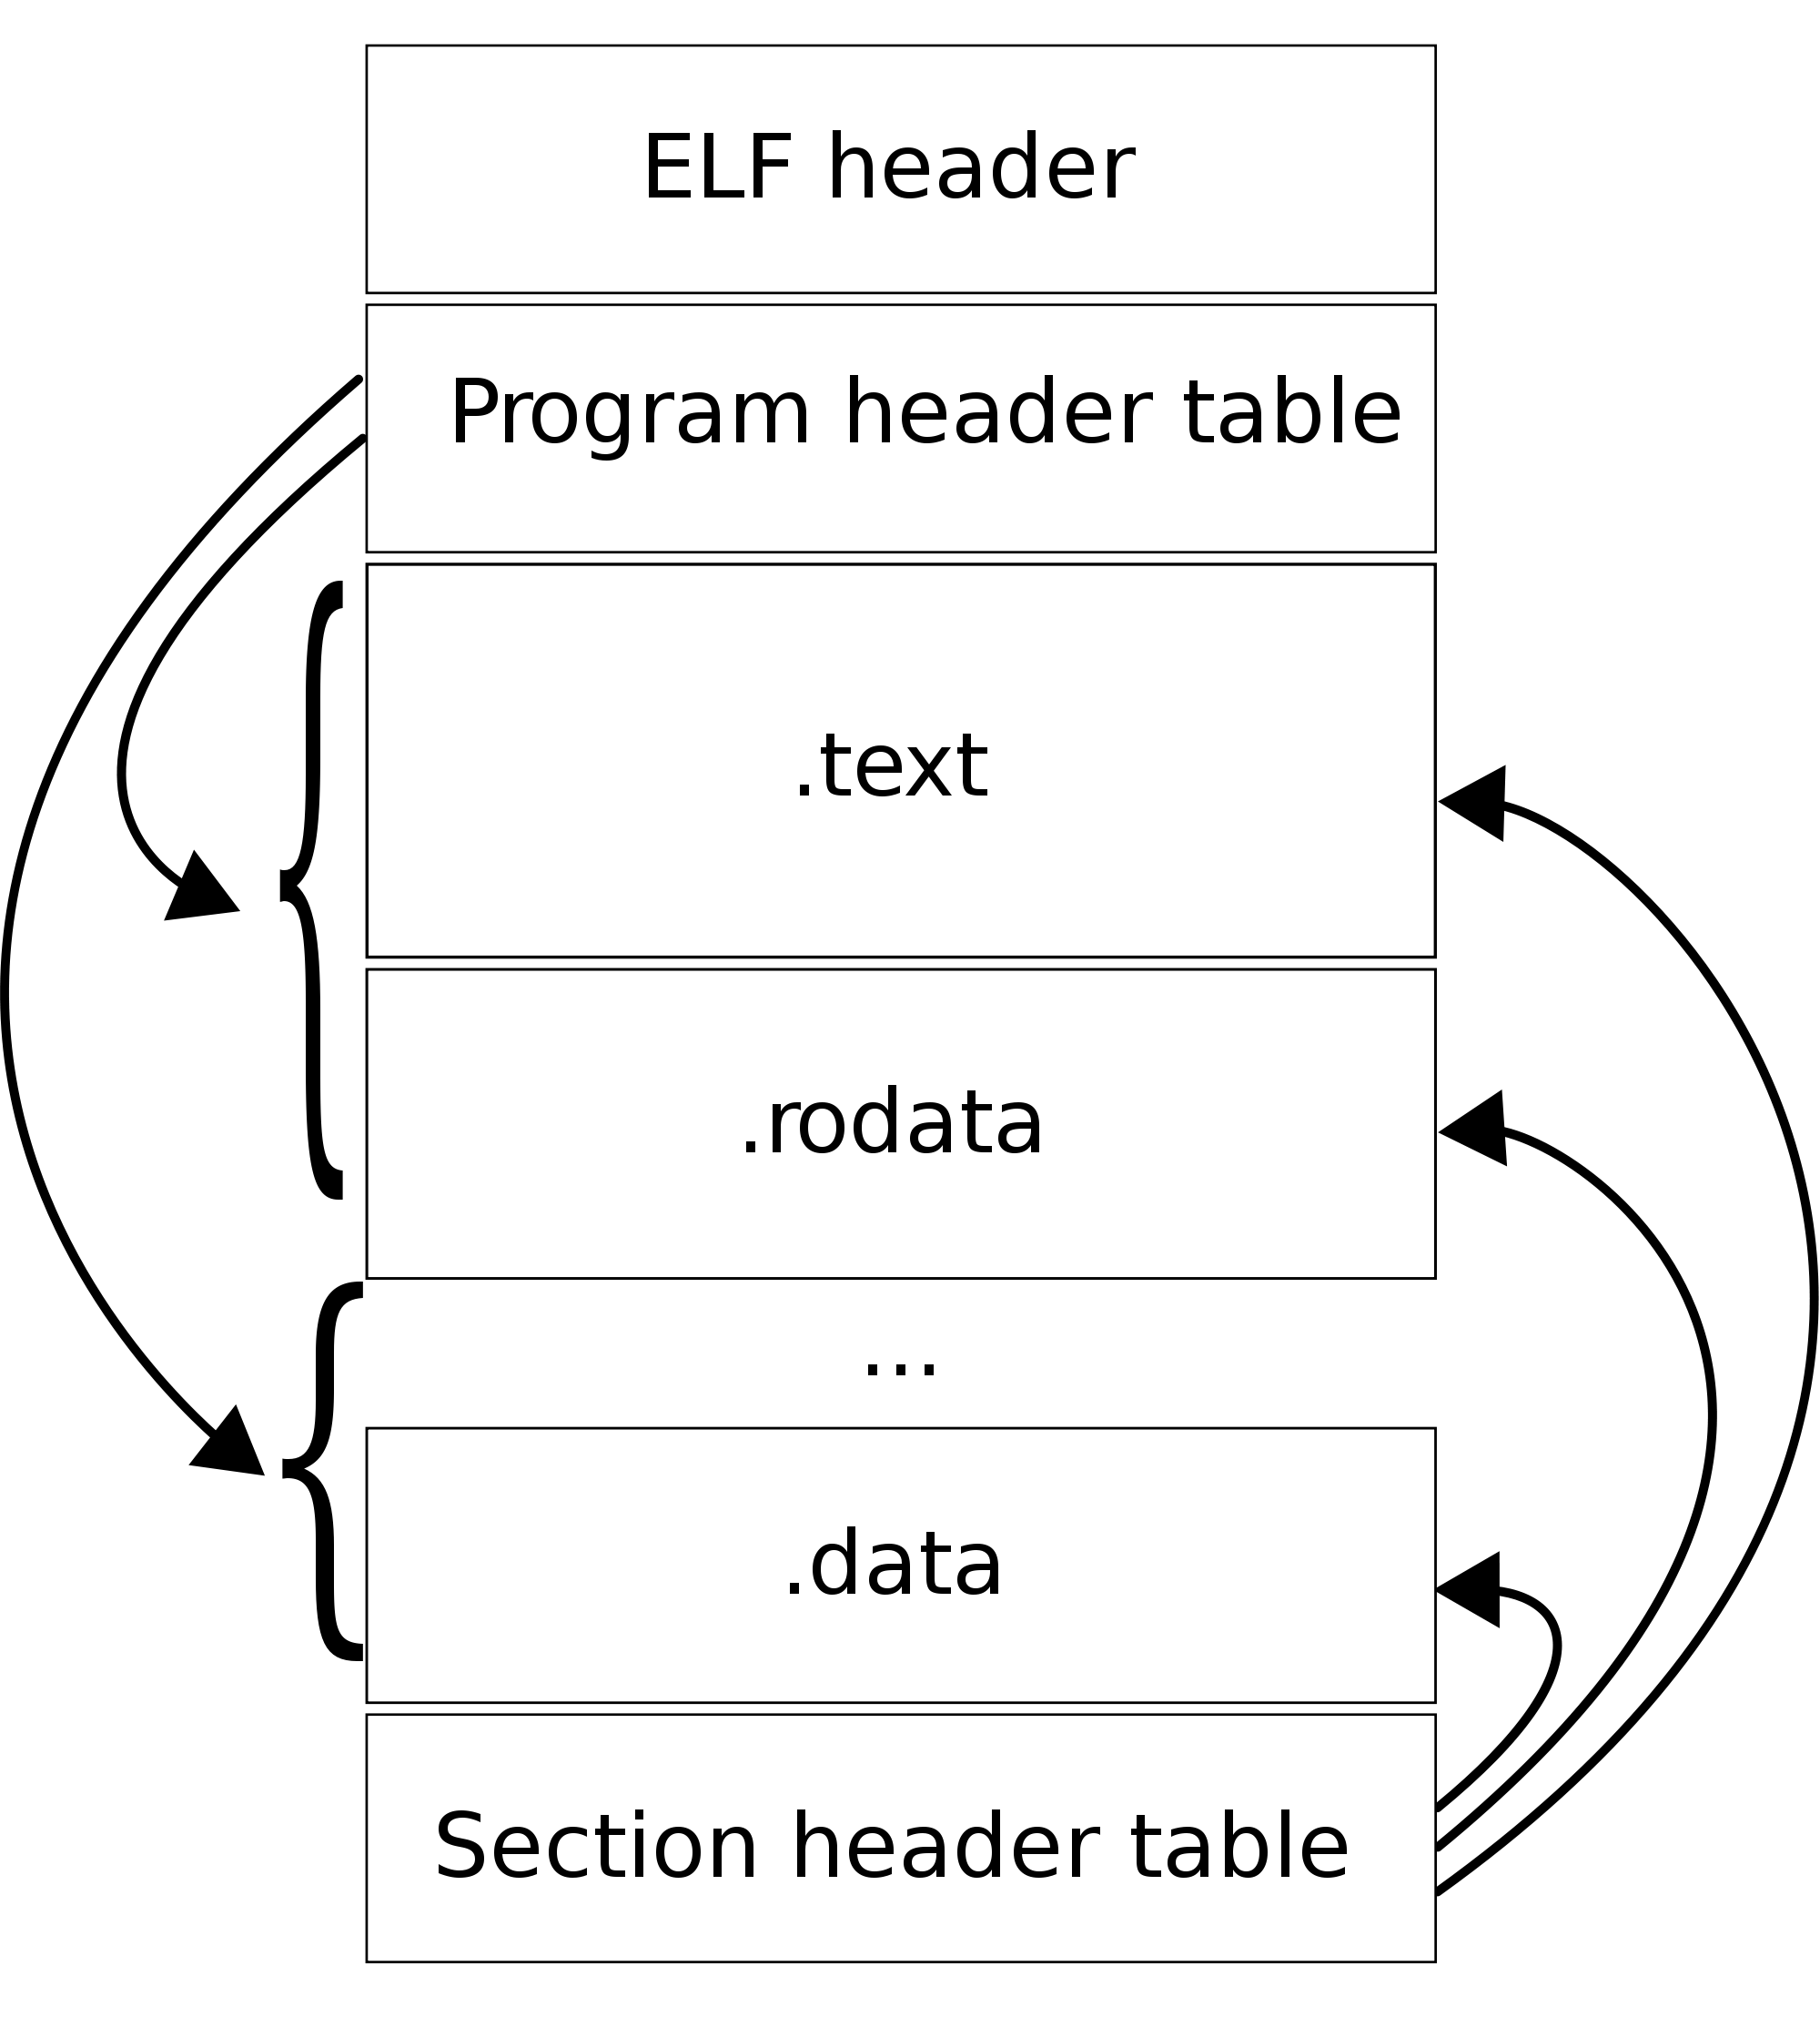
\includegraphics[height=0.8\textheight]{../../slides/elf-analysis/Elf-layout.png}
	\end{columns}
\end{frame}

\begin{frame}
	\frametitle{Структура ELF-файла}

	\begin{block}{readelf}
		Утилита для просмотра информации файлов в формате ELF.
	\end{block}

	\pause

	\begin{block}{Упражнение: просмотр программных заголовков}
		\begin{itemize}
			\item {\tt readelf -{}-file-header main-A\_B} -- интерпретация заголовка ELF-файла
			\item {\tt readelf -{}-sections main-A\_B} -- перечисление секций (для линковки)
			\item {\tt readelf -{}-segments main-A\_B} -- 
				перечисление программных сегментов (для исполнения)
			\item {\tt readelf -{}-symbols main-A\_B} -- список таблицы символов
		\end{itemize}
	\end{block}
\end{frame}

\begin{frame}
	\frametitle{Таблица символов}

	\begin{block}{strings}
		Утилита для получения символов из ELF-файла.
	\end{block}

	\begin{block}{nm}
		Утилита для получения символов из object файла.
	\end{block}

	\begin{block}{strip}
		Утилита для удаления символов из object файла.
	\end{block}
\end{frame}

\begin{frame}
	\frametitle{Таблица символов}

	\begin{block}{Упражнение}
		\begin{enumerate}
			\item {\tt strings main-A\_B}
			\item {\tt nm main-A\_B}
			\item {\tt nm -u main-A\_B}
			\item {\tt ls -l main-A\_B}
			\item {\tt strip main-A\_B}
			\item {\tt ls -l main-A\_B}
			\item {\tt nm main-A\_B}
			\item {\tt повторить предыдущее упражнение}
			\item Сделать выводы
		\end{enumerate}
	\end{block}

\end{frame}

}
\section{Binutils}
\mode<all>{%%
%% 

\begin{frame}
	\frametitle{objdump}

	\begin{block}{objdump}
		Утилита для просмотра информации по object файлам.
	\end{block}

	\pause

	\begin{block}{Упражнение}
		\begin{itemize}
			\item {\tt objdump -{}-file-headers main-A\_B} -- получить заголовок файла
			\item {\tt objdump -{}-section-headers main-A\_B} -- перечисление секций (для линковки)
			\item {\tt objdump -{}-syms main-A\_B} -- список таблицы символов
			\item {\tt objdump -{}-dynamic-syms main-A\_B} -- список динамических символов (как nm -u)
		\end{itemize}

	\end{block}
\end{frame}


\begin{frame}
	\frametitle{Дизассемблер objdump}

	\begin{block}{Упражнение: внутренниий мир программы}
		\begin{itemize}
			\item {\tt objdump -{}-disassemble main-A\_B} -- получить дизассемблированный файл
			\item {\tt objdump -{}-disassemble -j.text main-A\_B} -- 
				получить дизассемблированную исполняемую секцию {\tt .text}
			\item {\tt objdump -{}-disassemble -j.text -{}-file-offsets main-A\_B} -- 
				получить дизассемблированную исполняемую секцию {\tt .text} 
				и узнать где в файле располагаются инструкции
		\end{itemize}
	\end{block}
\end{frame}

\begin{frame}
	\frametitle{Что же наделал компилятор?}

	\begin{block}{Упражнение: анализируем вместе с исходником}
		\begin{itemize}
			\item Добавить в исходник {\tt main.c} объявление переменной и пустой цикл
			\item Добавить в {\tt Makefile} опции {\tt -g -O0}
			\item {\tt objdump -{}-source -{}-line-numbers main-A\_B}
			\item {\tt objdump -{}-source -{}-line-numbers -{}-file-offsets main.o}
			\item Изменить в {\tt Makefile} опцию {\tt -O0} на {\tt -O3}
			\item {\tt objdump -{}-source -{}-line-numbers -{}-file-offsets main.o}
			\item Сделать выводы ;-)
		\end{itemize}
	\end{block}
\end{frame}

}

\chapter{Отладка}
\mode<all>{\begin{frame}
  \frametitle{Инструменты отладки}
  \begin{itemize}
   \item printf
   \item Функциональный стиль + unit tests
   \item gdb
   \item valgrind
  \end{itemize}
\end{frame}
}
\section{Отладка с помощью printf}
\mode<all>{\begin{frame}
 \frametitle{Использование printf и логов}
 \begin{columns}
   \column{0.45\textwidth}
    \begin{center}
     Преимущества 
    \end{center}
    \begin{itemize}
     \item Работает везде и всегда
     \begin{itemize}
       \item В многопоточных программах
       \item При вызове из других программ
       \item Внутри ядра (printk)
       \item В реальном времени
       \item В разных языках
      \end{itemize}
    \end{itemize}
   \column{0.45\textwidth}
    \begin{center}
     Недостататки
    \end{center}
    \begin{itemize}
     \item Нужна перекомпиляция
     \item Нет интерактивности
     \item Нужно вычищать
     \item Трудно печатать сложные структуры
     \item Нет backtrace
    \end{itemize}
 \end{columns}
\end{frame}
}
\section{GNU отладчик gdb}
\mode<all>{\begin{frame}
  \frametitle{Базовые команды gdb}
  \begin{columns}
    \begin{column}{width=0.5\textwidth}
      \begin{itemize}
        \item help
        \item b (break)
        \item c (continue)
        \item s (step)
        \item p (print)
      \end{itemize}
    \end{column}
    \begin{column}{width=0.5\textwidth}
      \begin{itemize}
        \item bt (backtrace)
        \item finish
        \item return
        \item frame
      \end{itemize}
    \end{column}
  \end{columns}
\end{frame}
}
\section{Valgrind}
\mode<all>{%%
%% 
\begin{frame}
	\frametitle{Valgrind}

	\begin{block}{Valgrind Tools}
		\begin{enumerate}
			\item {\bf Memcheck} -- определяет ошибки при работе с памятью.
			\item {\bf Cachegrind} -- профайлер работы с кэшем и ветвлений.
			\item {\bf Callgrind} -- еще один кэш-профайлер.
			\item {\bf Helgrind} -- определяет ошибки в потоках.
			\item {\bf DRD} -- и еще один детектор ошибок в потоках.
			\item {\bf Massif} -- профайлер "кучи".
			\item {\bf DHAT} -- ...вы не поверите, но да, еще один.
			\item {\bf SGcheck} -- детектор работы со стеком и глобальными массивами.
			\item {\bf BBV} -- генератор блок-схем.
		\end{enumerate}
	\end{block}
\end{frame}
	
\begin{frame}
	\frametitle{Valgrind Memcheck}

	\begin{block}{Что умеет Memcheck}
		\begin{itemize}
			\item Утечки памяти
			\item Использование неинициализированной памяти
			\item Чтение/запись за пределами выделенной {\tt malloc} памяти
			\item Чтение/запись в некорректные области стека
			\item Использование неправильных пар вуделения/удаления блоков памяти:\\
				{\tt malloc/new/new[]} и {\tt free/delete/delete[]}
			\item Перекрытие участков памяти при использованиии {\tt memcpy()} и др.
%			\item "Злоупотребления" {\tt API pthreads}
		\end{itemize}
	\end{block}
\end{frame}

\begin{frame}[fragile]
	\frametitle{Упражнение: запуск}

	\begin{block}{Жертва}
	Да, опять {\tt Hello, World}!!!

	\end{block}

	\begin{block}{Компиляция}
		Флаги {\tt -g} и {\tt -O0}!

		Hint: {\tt export CFLAGS=''-g''}
	\end{block}

	\begin{block}{Запуск}
		{\tt valgrind ./prog}
	\end{block}

\end{frame}

\begin{frame}[fragile]
	\frametitle{Полезные опции}

	\begin{itemize}
		\item -{}-quiet VS -{}-verbose
		\item -{}-trace-children=yes -- дочерние процессы
		\item -{}-log-file=<logname>
		\item -{}-leak-check=full -- отслеживать утечки памяти 
		\item -{}-num-callers=<backtrace depth> -- глубина "размотки" стека
		\item -{}-track-fds=yes -- отслеживать незакрытые файлы
		\item -{}-track-origins=yes -- отслеживать происхождение неинициализированных значений\footnote{Дорогая операция}
		\item -{}-show-reachable=yes -- показывает неосвобожденную,  но неутекшую (есть ссылки из программы) память
		\item -{}-malloc-fill=val и -{}-free-fill=val -- заполняет память при вызовах malloc/free

	\end{itemize}

\end{frame}


		
\begin{frame}[fragile]
	\frametitle{Упражнение: некорректный указатель}

	\begin{lstlisting}
#include <stdlib.h>

main(void)
{
char *array;

    array = malloc(10*sizeof(char));
    array[10] = 'x';
    free( array);
    exit(0);
}
	\end{lstlisting}

	Пример: {\tt inv\_ptr.c}

\end{frame}

\begin{frame}[fragile]
	\frametitle{Упражнение: двойное освобождение памяти}

	\begin{lstlisting}
#include <stdlib.h>

main(void)
{
char *array;

    array = malloc(10*sizeof(char));
    free( array);
    free( array);
    exit(0);
}
	\end{lstlisting}

	Пример: {\tt dbl\_free.c}

\end{frame}



\begin{frame}[fragile]
	\frametitle{Упражнение: утечки памяти}

	\begin{lstlisting}
char *array;
int i;

for( i=0; i<100; i++)
    array = malloc(10*sizeof(char));

free( array);
	\end{lstlisting}

	\begin{block}{Детализация}
		{\tt -{}-leak-check=full}
	\end{block}

	Пример: {\tt leaks.c}

\end{frame}

\begin{frame}[fragile]
	\frametitle{Упражнение: объем выделенной памяти}

	\begin{lstlisting}
array = malloc(1<<31);
array[10000] = 0;
	\end{lstlisting}

	Пример: {\tt huge\_size.c}
	
	\bigskip
	\pause

	Задание:
	\begin{enumerate}
		\item изменить объем запрошенной памяти на больший, чем доступно в системе
	\end{enumerate}

\end{frame}

\begin{frame}[fragile]
	\frametitle{Упражнение: использование переменной вместо указателя}

	\begin{lstlisting}
    int i;
    scanf("%d", i);
	\end{lstlisting}

	Пример: {\tt inv\_type.c}
\end{frame}

\begin{frame}[fragile]
	\frametitle{Упражнение: неинициализированные переменные}

	\begin{lstlisting}
    int a;
    if ( a)
        {...};
	\end{lstlisting}

	Пример: {\tt uninit\_var.c}
\end{frame}

\begin{frame}[fragile]
	\frametitle{Макросы в исходниках}
	
	\begin{lstlisting}
#include <valgrind/valgrind.h>
	\end{lstlisting}

	\begin{itemize}
		\item {\tt RUNNING\_ON\_VALGRIND} -- возвращает 1, если запущено в Valgrind
		\item {\tt VALGRIND\_COUNT\_ERRORS} -- количество найденных ошибок
		\item {\tt VALGRIND\_PRINTF(format, ...)}
		\item {\tt VALGRIND\_PRINTF\_BACKTRACE(format, ...)}
	\end{itemize}

	\begin{lstlisting}
#include <valgrind/memcheck.h>
	\end{lstlisting}

	\begin{itemize}
		\item {\tt VALGRIND\_MAKE\_MEM\_NOACCESS( *addr, size)}
		\item {\tt VALGRIND\_DO\_LEAK\_CHECK} -- производит проверку утечки памяти
		\item для работы с собственным аллокатором:\\
		\begin{itemize}
			\item {\tt VALGRIND\_MALLOCLIKE\_BLOCK}
			\item {\tt VALGRIND\_FREELIKE\_BLOCK}
			\item {\tt VALGRIND\_RESIZEINPLACE\_BLOCK}
		\end{itemize}
	\end{itemize}


\end{frame}

\begin{frame}[fragile]
	\frametitle{Упражнение: пример использования макроса}

	\begin{lstlisting}
void dobug(char *addr){
  char *local = addr;
  local[4]=32;
}

main(void) {
  char addr[]="Hello,  world!!!";
  printf("%s\n",  addr);
  dobug( addr);
  printf("%s\n",  addr);
  return (0);
}
	\end{lstlisting}

%	Пример: {\tt uninit\_addr.c}

	\begin{block}{Задание}
		Добавить макрос {\tt VALGRIND\_MAKE\_MEM\_NOACCESS()} перед вызовом {\tt dobug()}.
	\end{block}

\end{frame}


\begin{frame}[fragile]
	\frametitle{GDB + Valgrind}

	Valgrind запускет программы на "синтетическом" процессоре, поэтому GDB не работает!

	Для отладки используется {\tt vgdb}: \\

	\begin{verbatim}
valgrind --vgdb=yes --vgdb-error=0 prog
	\end{verbatim}


	а {\tt gdb} запустить:
	\begin{verbatim}
gdb prog
(gdb) target remote | vgdb
	\end{verbatim}

	\pause
	\begin{block}{Упражнение}
		Попробовать провести отладку программы {\tt segfault.c} с помощью связки Valgrind и GDB.
	\end{block}
\end{frame}



}
\section{Отладка системных вызовов (strace,ltrace)}
\mode<all>{% Copyright (C) 2012-2014  Denis Pynkin <denis_pynkin@epam.com>
% Copyright (C) 2012-2014  Yury Adamov  <yury_adamov@epam.com>

% Copyright (C) 2012-2013  Dmitry V. Levin <ldv@altlinux.org>
% Permission is granted to copy, distribute and/or modify this document
% under the terms of the GNU Free Documentation License, Version 1.2
% or any later version published by the Free Software Foundation;
% with no Invariant Sections, no Front-Cover Texts, and no Back-Cover Texts.


\begin{frame}[fragile]
  \frametitle{strace, ltrace}
  \begin{center}
   Основные опции 
  \end{center}
  \begin{itemize}
   \item \texttt{-e <expression>}
\begin{lstlisting}[language=sh]
  strace -e read,write -e read=50 
\end{lstlisting}
   \item \texttt{-p <pid>}
\begin{lstlisting}[language=sh]
  ltrace -p 1021
\end{lstlisting}
   \item \texttt{-c}
   \item \texttt{-f} следить за дочерними процессами
   \item \texttt{-o <filename>}
   \item \texttt{-t, -T}
  \end{itemize}
\end{frame}

\begin{frame}
\frametitle{Более полный набор опций -e}

\begin{itemize}
\item \texttt{trace=<smth>}
    \begin{itemize}
    \item file
    \item process
    \item network
    \item signal
    \end{itemize}
\item \texttt{read=<smth>} 
\item \texttt{write=<smth>}
\item \texttt{raw=<smth>}
\end{itemize}
\end{frame}

\begin{frame}
 \frametitle{Некоторые возможные применения}
 \begin{itemize}
  \item Обнаружение файлов, открываемых приложением (\texttt{-e open})
    \begin{itemize}
      \item библиотек, подключаемых в реальном времени
      \item конфигурационных файлов
    \end{itemize}
   \item Обнаружение сетевых соединений \texttt{connect, accept, recvfrom, sendto, poll, read, write} 
   \item Чем занято приложение в текущий момент
   \item Почему приложение сейчас тормозит
   \item Профилирование
   \item Получение дампов записей в устройства, сокеты и т.п.
 \end{itemize}
\end{frame}

%\begin{frame}
% \frametitle{Упражнение}
% \begin{enumerate}
%   \item Выяснить, какие конфигурационные файлы пытается открыть \texttt{vim}
%   \item В каком системном вызове проводит больше всего времени \texttt{ls /usr/bin/}. То же для \texttt{ls -l /usr/bin}
%   \item Повторить предыдущий пункт для библиотечных вызовов.
%   \item Попробовать различные представления времени: {\tt -r}, {\tt -t},{\tt -tt},{\tt -ttt}.
% \end{enumerate}
%\end{frame}

\begin{frame}[fragile]{strace usage examples: -P, -e trace=file}
\scriptsize
\begin{verbatim}
$ strace -e file ls /var/empty
execve("/bin/ls", ["ls", "/var/empty"], [/* 32 vars */]) = 0
access("/etc/ld.so.preload", R_OK)      = -1 ENOENT (No such file or directory)
open("/etc/ld.so.cache", O_RDONLY)      = 3
open("/lib64/libtinfo.so.5", O_RDONLY)  = 3
open("/lib64/libselinux.so.1", O_RDONLY) = 3
open("/lib64/librt.so.1", O_RDONLY)     = 3
open("/lib64/libcap.so.2", O_RDONLY)    = 3
open("/lib64/libacl.so.1", O_RDONLY)    = 3
open("/lib64/libc.so.6", O_RDONLY)      = 3
open("/lib64/libdl.so.2", O_RDONLY)     = 3
open("/lib64/libpthread.so.0", O_RDONLY) = 3
open("/lib64/libattr.so.1", O_RDONLY)   = 3
stat("/var/empty", {st_mode=S_IFDIR|0555, st_size=4096, ...}) = 0
open("/var/empty", O_RDONLY|O_NONBLOCK|O_DIRECTORY|O_CLOEXEC) = 3
+++ exited with 0 +++
\end{verbatim}

\begin{verbatim}
$ strace -P /etc/ld.so.cache ls /var/empty
open("/etc/ld.so.cache", O_RDONLY)      = 3
fstat(3, {st_mode=S_IFREG|0644, st_size=22446, ...}) = 0
mmap(NULL, 22446, PROT_READ, MAP_PRIVATE, 3, 0) = 0x2b7ac2ba9000
close(3)                                = 0
+++ exited with 0 +++
\end{verbatim}
\end{frame}

\begin{frame}[fragile]{strace usage examples: -P, -v}
\scriptsize
\begin{verbatim}
$ strace -P /var/empty ls /var/empty
stat("/var/empty", {st_mode=S_IFDIR|0555, st_size=4096, ...}) = 0
open("/var/empty", O_RDONLY|O_NONBLOCK|O_DIRECTORY|O_CLOEXEC) = 3
fcntl(3, F_GETFD)                       = 0x1 (flags FD_CLOEXEC)
getdents(3, /* 2 entries */, 32768)     = 48
getdents(3, /* 0 entries */, 32768)     = 0
close(3)                                = 0
+++ exited with 0 +++
\end{verbatim}

\begin{verbatim}
$ strace -P /var/empty -v ls /var/empty
stat("/var/empty", {st_dev=makedev(0, 30), st_ino=1020461,
  st_mode=S_IFDIR|0555, st_nlink=2, st_uid=0, st_gid=0, st_blksize=4096,
  st_blocks=8, st_size=4096, st_atime=2012/07/22-14:21:04,
  st_mtime=2012/05/17-19:22:58, st_ctime=2012/05/17-19:24:07}) = 0
open("/var/empty", O_RDONLY|O_NONBLOCK|O_DIRECTORY|O_CLOEXEC) = 3
fcntl(3, F_GETFD)                       = 0x1 (flags FD_CLOEXEC)
getdents(3, {{d_ino=799280, d_off=1551270678, d_reclen=24, d_name=".."}
  {d_ino=1020461, d_off=2147483647, d_reclen=24, d_name="."}}, 32768) = 48
getdents(3, {}, 32768)                  = 0
close(3)                                = 0
+++ exited with 0 +++
\end{verbatim}
\end{frame}

\begin{frame}[fragile]{strace usage examples: -y, -e trace=}
\scriptsize
%\tiny
\begin{verbatim}
$ strace -e fstat,close -y ls /var/empty >/dev/null
fstat(3</etc/ld.so.cache>, {st_mode=S_IFREG|0644, st_size=22446, ...}) = 0
close(3</etc/ld.so.cache>)              = 0
fstat(3</lib/libtinfo.so.5.7>, {st_mode=S_IFREG|0644, st_size=135352, ...}) = 0
close(3</lib/libtinfo.so.5.7>)        = 0
fstat(3</lib/libselinux.so.1>, {st_mode=S_IFREG|0644, st_size=121992, ...}) = 0
close(3</lib/libselinux.so.1>)        = 0
fstat(3</lib/librt-2.11.3.so>, {st_mode=S_IFREG|0755, st_size=31792, ...}) = 0
close(3</lib/librt-2.11.3.so>)        = 0
fstat(3</lib/libcap.so.2.16>, {st_mode=S_IFREG|0644, st_size=23048, ...}) = 0
close(3</lib/libcap.so.2.16>)         = 0
fstat(3</lib/libacl.so.1.1.0>, {st_mode=S_IFREG|0644, st_size=35376, ...}) = 0
close(3</lib/libacl.so.1.1.0>)        = 0
fstat(3</lib/libc-2.11.3.so>, {st_mode=S_IFREG|0755, st_size=1452024, ...}) = 0
close(3</lib/libc-2.11.3.so>)         = 0
fstat(3</lib/libdl-2.11.3.so>, {st_mode=S_IFREG|0755, st_size=14776, ...}) = 0
close(3</lib/libdl-2.11.3.so>)        = 0
fstat(3</lib/libpthread-2.11.3.so>, {st_mode=S_IFREG|0755, st_size=138064, ...}) = 0
close(3</lib/libpthread-2.11.3.so>)   = 0
fstat(3</lib/libattr.so.1.1.0>, {st_mode=S_IFREG|0644, st_size=18704, ...}) = 0
close(3</lib/libattr.so.1.1.0>)       = 0
close(3</var/empty>)                    = 0
close(1</dev/null>)                     = 0
close(2</dev/pts/0>)                    = 0
+++ exited with 0 +++
\end{verbatim}
\end{frame}

\begin{frame}[fragile]{strace usage examples: -y, -e trace=, -e read=}
\Tiny
\begin{verbatim}
$ strace -e trace=read -e read=3 -y ls /var/empty
read(3</lib64/libtinfo.so.5.7>, "\177ELF\2\1\1\0\0\0\0\0\0\0\0\0\3\0>\0\1\0\0\0\300\315\0\0\0\0\0\0"..., 832) = 832
 | 00000  7f 45 4c 46 02 01 01 00  00 00 00 00 00 00 00 00  .ELF.... ........ |
 | 00010  03 00 3e 00 01 00 00 00  c0 cd 00 00 00 00 00 00  ..>..... ........ |
 | 00320  00 00 00 00 00 00 00 00  00 00 00 00 4d 00 00 00  ........ ....M... |
 | 00330  00 00 00 00 00 00 00 00  00 00 00 00 00 00 00 00  ........ ........ |
read(3</lib64/libselinux.so.1>, "\177ELF\2\1\1\0\0\0\0\0\0\0\0\0\3\0>\0\1\0\0\0\240W\0\0\0\0\0\0"..., 832) = 832
 | 00000  7f 45 4c 46 02 01 01 00  00 00 00 00 00 00 00 00  .ELF.... ........ |
 | 00010  03 00 3e 00 01 00 00 00  a0 57 00 00 00 00 00 00  ..>..... .W...... |
 | 00320  40 20 00 00 20 00 00 80  c8 84 e2 00 00 12 00 03  @ .. ... ........ |
 | 00330  20 40 02 21 80 50 02 21  70 00 00 00 71 00 00 00   @.!.P.! p...q... |
read(3</lib64/librt-2.11.3.so>, "\177ELF\2\1\1\0\0\0\0\0\0\0\0\0\3\0>\0\1\0\0\0\200!\0\0\0\0\0\0"..., 832) = 832
 | 00000  7f 45 4c 46 02 01 01 00  00 00 00 00 00 00 00 00  .ELF.... ........ |
 | 00010  03 00 3e 00 01 00 00 00  80 21 00 00 00 00 00 00  ..>..... .!...... |
 | 00320  00 00 00 00 00 00 00 00  00 00 00 00 00 00 00 00  ........ ........ |
 | 00330  00 00 00 00 48 00 00 00  00 00 00 00 49 00 00 00  ....H... ....I... |
read(3</lib64/libcap.so.2.16>, "\177ELF\2\1\1\0\0\0\0\0\0\0\0\0\3\0>\0\1\0\0\0@\30\0\0\0\0\0\0"..., 832) = 832
 | 00000  7f 45 4c 46 02 01 01 00  00 00 00 00 00 00 00 00  .ELF.... ........ |
 | 00010  03 00 3e 00 01 00 00 00  40 18 00 00 00 00 00 00  ..>..... @....... |
 | 00320  89 71 ee b2 ee 3e 3c d4  dd e7 a8 99 18 bf 5b 17  .q...><. ......[. |
 | 00330  7d dd 81 63 ed 16 0b 88  4d a7 3a ea f5 3e 3c d4  }..c.... M.:..><. |
read(3</lib64/libacl.so.1.1.0>, "\177ELF\2\1\1\0\0\0\0\0\0\0\0\0\3\0>\0\1\0\0\0\240\37\0\0\0\0\0\0"..., 832) = 832
 | 00000  7f 45 4c 46 02 01 01 00  00 00 00 00 00 00 00 00  .ELF.... ........ |
 | 00010  03 00 3e 00 01 00 00 00  a0 1f 00 00 00 00 00 00  ..>..... ........ |
 | 00320  47 00 00 00 00 00 00 00  48 00 00 00 4a 00 00 00  G....... H...J... |
 | 00330  00 00 00 00 4b 00 00 00  00 00 00 00 00 00 00 00  ....K... ........ |
read(3</lib64/libc-2.11.3.so>, "\177ELF\2\1\1\3\0\0\0\0\0\0\0\0\3\0>\0\1\0\0\0\360\354\1\0\0\0\0\0"..., 832) = 832
 | 00000  7f 45 4c 46 02 01 01 03  00 00 00 00 00 00 00 00  .ELF.... ........ |
 | 00010  03 00 3e 00 01 00 00 00  f0 ec 01 00 00 00 00 00  ..>..... ........ |
 | 00320  80 ca 44 42 28 00 06 80  10 18 42 00 20 40 80 00  ..DB(... ..B. @.. |
 | 00330  09 50 00 51 8a 40 10 00  00 00 00 08 00 00 11 10  .P.Q.@.. ........ |
read(3</lib64/libdl-2.11.3.so>, "\177ELF\2\1\1\0\0\0\0\0\0\0\0\0\3\0>\0\1\0\0\0\340\r\0\0\0\0\0\0"..., 832) = 832
 | 00000  7f 45 4c 46 02 01 01 00  00 00 00 00 00 00 00 00  .ELF.... ........ |
 | 00010  03 00 3e 00 01 00 00 00  e0 0d 00 00 00 00 00 00  ..>..... ........ |
 | 00320  91 21 fc f8 06 02 04 f9  fb 33 fb 0f f9 19 73 42  .!...... .3....sB |
 | 00330  fa 19 73 42 95 b3 5f 19  7f 9e d0 18 61 a2 92 06  ..sB.._. ....a... |
read(3</lib64/libpthread-2.11.3.so>, "\177ELF\2\1\1\0\0\0\0\0\0\0\0\0\3\0>\0\1\0\0\0\360Y\0\0\0\0\0\0"..., 832) = 832
 | 00000  7f 45 4c 46 02 01 01 00  00 00 00 00 00 00 00 00  .ELF.... ........ |
 | 00010  03 00 3e 00 01 00 00 00  f0 59 00 00 00 00 00 00  ..>..... .Y...... |
 | 00320  01 05 00 50 20 a9 02 07  28 00 00 82 04 98 40 04  ...P ... (.....@. |
 | 00330  00 10 e0 54 00 02 40 02  02 10 c1 30 44 02 80 00  ...T..@. ...0D... |
read(3</lib64/libattr.so.1.1.0>, "\177ELF\2\1\1\0\0\0\0\0\0\0\0\0\3\0>\0\1\0\0\0\260\23\0\0\0\0\0\0"..., 832) = 832
 | 00000  7f 45 4c 46 02 01 01 00  00 00 00 00 00 00 00 00  .ELF.... ........ |
 | 00010  03 00 3e 00 01 00 00 00  b0 13 00 00 00 00 00 00  ..>..... ........ |
 | 00320  bf a8 e3 f8 db 0c 16 89  bb e3 92 7c c5 e8 1b 9b  ........ ...|.... |
 | 00330  05 c1 58 15 4b 3d 47 f3  91 78 a9 dd eb d3 ef 0e  ..X.K=G. .x...... |
+++ exited with 0 +++
\end{verbatim}
\end{frame}

\begin{frame}[fragile]{strace usage examples: -r, -e trace=process}
\scriptsize
\begin{verbatim}
$ strace -r /bin/true
     0.000000 execve("/bin/true", ["/bin/true"], [/* 32 vars */]) = 0
     0.000281 exit_group(0)             = ?
     0.000063 +++ exited with 0 +++
\end{verbatim}

\begin{verbatim}
# strace -r -e process unshare -i /bin/true
     0.000000 execve("/usr/bin/unshare",
       ["/usr/bin/unshare", "-i", "/bin/true"], [/* 32 vars */]) = 0
     0.000899 arch_prctl(ARCH_SET_FS, 0x7f4e537cd700) = 0
     0.000398 unshare(CLONE_NEWIPC)     = 0
     0.000190 execve("/bin/true", ["/bin/true"], [/* 32 vars */]) = 0
     0.000186 exit_group(0)             = ?
     0.028931 +++ exited with 0 +++
\end{verbatim}
\end{frame}

\begin{frame}[fragile]{strace usage examples: -r, -T, -f, -e trace=process}
\Tiny
\begin{verbatim}
$ strace -e process -r -T sh -c 'kill $$'
     0.000000 execve("/bin/sh", ["sh", "-c", "kill $$"], [/* 32 vars */]) = 0 <0.000361>
     0.001185 arch_prctl(ARCH_SET_FS, 0x2b0c3236b020) = 0 <0.000008>
     0.002239 --- SIGTERM {si_signo=SIGTERM, si_code=SI_USER, si_pid=12345, si_uid=500} ---
     0.000218 +++ killed by SIGTERM +++
\end{verbatim}

\begin{verbatim}
$ strace -e process -f -q \
 sh -c 'sleep 1 & pid=$!; sleep 0.1; kill $pid; wait'
execve("/bin/sh", ["sh", "-c", "sleep 1 & pid=$!; sleep 0.1; kil"...], [/* 32 vars */]) = 0
arch_prctl(ARCH_SET_FS, 0x2ae37beef020) = 0
clone(child_stack=0, flags=CLONE_CHILD_CLEARTID|CLONE_CHILD_SETTID|SIGCHLD, child_tidptr=0x2ae37beef2f0) = 10001
[pid 10000] clone(child_stack=0, flags=CLONE_CHILD_CLEARTID|CLONE_CHILD_SETTID|SIGCHLD, child_tidptr=0x2ae37beef2f0) = 10002
[pid 10001] execve("/bin/sleep", ["sleep", "1"], [/* 32 vars */] <unfinished ...>
[pid 10002] execve("/bin/sleep", ["sleep", "0.1"], [/* 32 vars */] <unfinished ...>
[pid 10001] <... execve resumed> )      = 0
[pid 10002] <... execve resumed> )      = 0
[pid 10000] wait4(-1,  <unfinished ...>
[pid 10001] arch_prctl(ARCH_SET_FS, 0x2b8cf7d49b20) = 0
[pid 10002] arch_prctl(ARCH_SET_FS, 0x2ada74416b20) = 0
[pid 10002] exit_group(0)               = ?
[pid 10002] +++ exited with 0 +++
[pid 10000] <... wait4 resumed> [{WIFEXITED(s) && WEXITSTATUS(s) == 0}], 0, NULL) = 10002
[pid 10000] --- SIGCHLD {si_signo=SIGCHLD, si_code=CLD_EXITED, si_pid=10002, si_status=0, si_utime=0, si_stime=0} ---
[pid 10000] wait4(-1, 0x7fff7560e53c, WNOHANG, NULL) = 0
[pid 10001] --- SIGTERM {si_signo=SIGTERM, si_code=SI_USER, si_pid=10000, si_uid=600} ---
[pid 10001] +++ killed by SIGTERM +++
--- SIGCHLD {si_signo=SIGCHLD, si_code=CLD_KILLED, si_pid=10001, si_status=SIGTERM, si_utime=1, si_stime=0} ---
wait4(-1, [{WIFSIGNALED(s) && WTERMSIG(s) == SIGTERM}], WNOHANG, NULL) = 10001
wait4(-1, 0x7fff7560e58c, WNOHANG, NULL) = -1 ECHILD (No child processes)
exit_group(0)                           = ?
+++ exited with 0 +++
\end{verbatim}
\end{frame}

\begin{frame}[fragile]{strace usage examples: -ff, -ttt, -o, strace-log-merge}
\Tiny
\begin{verbatim}
$ strace -e process -ff -ttt -o log \ 
  sh -c 'sleep 1 & pid=$!; sleep 0.1; kill $pid; wait'
sh: line 1: 10001 Terminated              sleep 1
\end{verbatim}

\begin{verbatim}
$ head -1 log.*
==> log.10000 <==
1342993484.722384 execve("/bin/sh", ["sh", "-c", "sleep 1 & pid=$!; sleep 0.1; kil"...], [/* 32 vars */]) = 0
==> log.10001 <==
1342993484.727498 execve("/bin/sleep", ["sleep", "1"], [/* 32 vars */]) = 0
==> log.10002 <==
1342993484.727422 execve("/bin/sleep", ["sleep", "0.1"], [/* 32 vars */]) = 0
\end{verbatim}

\begin{verbatim}
$ strace-log-merge log
10000 1342993484.722384 execve("/bin/sh", ["sh", "-c", "sleep 1 & pid=$!; sleep 0.1; kil"...], [/* 33 vars */]) = 0
10000 1342993484.723369 arch_prctl(ARCH_SET_FS, 0x2ad5cc1fa020) = 0
10000 1342993484.725378 clone(child_stack=0, flags=CLONE_CHILD_CLEARTID|CLONE_CHILD_SETTID|SIGCHLD,
  child_tidptr=0x2ad5cc1fa2f0) = 10001
10000 1342993484.726783 clone(child_stack=0, flags=CLONE_CHILD_CLEARTID|CLONE_CHILD_SETTID|SIGCHLD,
  child_tidptr=0x2ad5cc1fa2f0) = 10002
10000 1342993484.727188 wait4(-1, [{WIFEXITED(s) && WEXITSTATUS(s) == 0}], 0, NULL) = 10002
10002 1342993484.727422 execve("/bin/sleep", ["sleep", "0.1"], [/* 32 vars */]) = 0
10001 1342993484.727498 execve("/bin/sleep", ["sleep", "1"], [/* 32 vars */]) = 0
10002 1342993484.769744 arch_prctl(ARCH_SET_FS, 0x2acee796db20) = 0
10001 1342993484.769845 arch_prctl(ARCH_SET_FS, 0x2b2bd019cb20) = 0
10002 1342993484.872233 exit_group(0)         = ?
10002 1342993484.872389 +++ exited with 0 +++
10000 1342993484.872492 --- SIGCHLD {si_signo=SIGCHLD, si_code=CLD_EXITED, si_pid=10002, si_status=0, si_utime=0,
  si_stime=0} ---
10000 1342993484.872519 wait4(-1, 0x7fffe27a860c, WNOHANG, NULL) = 0
10001 1342993484.872666 --- SIGTERM {si_signo=SIGTERM, si_code=SI_USER, si_pid=10000, si_uid=600} ---
10000 1342993484.872795 wait4(-1, [{WIFSIGNALED(s) && WTERMSIG(s) == SIGTERM}], 0, NULL) = 10001
10001 1342993484.872849 +++ killed by SIGTERM +++
10000 1342993484.873117 --- SIGCHLD {si_signo=SIGCHLD, si_code=CLD_KILLED, si_pid=10001, si_status=SIGTERM,
  si_utime=0, si_stime=0} ---
10000 1342993484.873140 wait4(-1, 0x7fffe27a81bc, WNOHANG, NULL) = -1 ECHILD (No child processes)
10000 1342993484.873339 exit_group(0)         = ?
10000 1342993484.873599 +++ exited with 0 +++
\end{verbatim}
\end{frame}

\begin{frame}[fragile]{strace usage examples: -o pipeline}
\scriptsize
\begin{verbatim}
$ strace -e open -o '|grep /lib' ls /var/empty
open("/lib64/libtinfo.so.5", O_RDONLY)  = 3
open("/lib64/libselinux.so.1", O_RDONLY) = 3
open("/lib64/librt.so.1", O_RDONLY)     = 3
open("/lib64/libcap.so.2", O_RDONLY)    = 3
open("/lib64/libacl.so.1", O_RDONLY)    = 3
open("/lib64/libc.so.6", O_RDONLY)      = 3
open("/lib64/libdl.so.2", O_RDONLY)     = 3
open("/lib64/libpthread.so.0", O_RDONLY) = 3
open("/lib64/libattr.so.1", O_RDONLY)   = 3
\end{verbatim}

\begin{verbatim}
$ strace -e desc -y -o "|grep '</[^l]'" ls /var/empty
fstat(3</etc/ld.so.cache>, {st_mode=S_IFREG|0644, st_size=22446, ...}) = 0
mmap(NULL, 22446, PROT_READ, MAP_PRIVATE, 3</etc/ld.so.cache>, 0) = 0x2ab097dfb000
close(3</etc/ld.so.cache>)              = 0
ioctl(1</dev/pts/0>, SNDCTL_TMR_TIMEBASE or SNDRV_TIMER_IOCTL_NEXT_DEVICE or TCGETS, {B38400 opost isig icanon echo ...}) = 0
ioctl(1</dev/pts/0>, TIOCGWINSZ, {ws_row=46, ws_col=128, ws_xpixel=1408, ws_ypixel=828}) = 0
fcntl(3</var/empty>, F_GETFD)           = 0x1 (flags FD_CLOEXEC)
getdents(3</var/empty>, /* 2 entries */, 32768) = 48
getdents(3</var/empty>, /* 0 entries */, 32768) = 0
close(3</var/empty>)                    = 0
close(1</dev/pts/0>)                    = 0
close(2</dev/pts/0>)                    = 0
\end{verbatim}
\end{frame}

\begin{frame}[fragile]{strace usage examples: -p}
\begin{verbatim}
$ sleep 1 & sleep 1 & sleep 0.1 &&
  strace -e process -p "$(pidof sleep)"
[1] 10000
[2] 10001
Process 10001 attached
Process 10000 attached
[pid 10000] exit_group(0)               = ?
[pid 10001] exit_group(0)               = ?
[pid 10001] +++ exited with 0 +++
[2]+  Done                    sleep 1
+++ exited with 0 +++
[1]-  Done                    sleep 1

\end{verbatim}
\end{frame}

\begin{frame}[fragile]{strace usage examples: -c, -S}
\tiny
\begin{verbatim}
$ strace -c -S calls find /usr/share/doc/ > /dev/null 
% time     seconds  usecs/call     calls    errors syscall
------ ----------- ----------- --------- --------- ----------------
  1.77    0.000023           0      6417         1 fcntl
  1.85    0.000024           0      1992           close
 93.83    0.001216           1       982           getdents
  1.70    0.000022           0       982           newfstatat
  0.00    0.000000           0       520           fstat
  0.85    0.000011           0       511           openat
  0.00    0.000000           0        60           write
  0.00    0.000000           0        23           mmap
  0.00    0.000000           0        14           mprotect
  0.00    0.000000           0         9           open
  0.00    0.000000           0         8           read
  0.00    0.000000           0         6           brk
  0.00    0.000000           0         6           fadvise64
  0.00    0.000000           0         3           munmap
  0.00    0.000000           0         3         2 ioctl
  0.00    0.000000           0         2           rt_sigaction
  0.00    0.000000           0         2         1 futex
  0.00    0.000000           0         1           rt_sigprocmask
  0.00    0.000000           0         1         1 access
  0.00    0.000000           0         1           execve
  0.00    0.000000           0         1           uname
  0.00    0.000000           0         1           fchdir
  0.00    0.000000           0         1           gettimeofday
  0.00    0.000000           0         1           getrlimit
  0.00    0.000000           0         1           statfs
  0.00    0.000000           0         1           arch_prctl
  0.00    0.000000           0         1           set_tid_address
  0.00    0.000000           0         1           set_robust_list
------ ----------- ----------- --------- --------- ----------------
100.00    0.001296                 11551         5 total
\end{verbatim}
\end{frame}


}
\section{Просмотр списка вызовов функций (backtrace)}
\mode<all>{%%
%% 
\begin{frame}[fragile]
	\frametitle{Встроенные функции gcc}

	\begin{block}{Адрес возврата ({\tt gcc})}
		
		Встроенные в {\tt gcc} функции для получения адреса вызывающей функции:

	\begin{lstlisting}
void * __builtin_return_address (unsigned int level);
	\end{lstlisting}
	\end{block}

	\begin{block}{Пример}
	
	Добавить в функцию {\tt second()} код:

	\begin{lstlisting}
printf("Frame 0: %p\n",  __builtin_return_address(0));
printf("Frame 1: %p\n",  __builtin_return_address(1));
printf("Frame 2: %p\n",  __builtin_return_address(2));
printf("Frame 3: %p\n",  __builtin_return_address(3));
	\end{lstlisting}
	\end{block}

\end{frame}

\begin{frame}[fragile]
	\frametitle{{\tt addr2line}}

	\begin{block}{Перевод адреса в строку}
		{\tt addr2line <address>}

		\begin{itemize}
			\item {\tt -e filename} -- бинарный файл
			\item {\tt -f} -- показать имена функций 
			\item {\tt -i} -- для inline функций -- показывать первую не встроенную
			\item {\tt -C} -- нормальные имена для "искалеченных" (C++) функций
		\end{itemize}
	\end{block}

	\begin{block}{Упражнение}

		\begin{itemize}
			\item Вызвать {\tt addr2line}, передав туда адреса, полученные из {\tt \_\_builtin\_return\_address()}.
			\item Перекомпилировать с флагом {\tt -g}
			\item Повторить вызов {\tt addr2line}
		\end{itemize}

	\end{block}

\end{frame}

%\begin{frame}[fragile]
%	\frametitle{Пример}
%
%	\begin{block}{Вывод {\tt backtrace}}
%	\begin{verbatim}
%./backtrace() [0x400c3e]
%/lib64/libc.so.6(+0x350f0) [0x7fb5711450f0]
%./backtrace(fill_random_ascii_buffer+0x40) [0x400d11]
%./backtrace(main+0xc9) [0x400dfe]
%	\end{verbatim}
%
%	\end{block}
%	\begin{block}{Вызов {\tt addr2line}}
%	\begin{verbatim}
%addr2line -e backtrace -ifC 0x400c3e
%	\end{verbatim}
%
%	\end{block}
%
%\end{frame}

\begin{frame}[fragile]
	\frametitle{Добавим ошибку}

	\begin{block}{Ошибка}
	
	\begin{lstlisting}
void second (void) {
  char *buf;
  sprintf( buf, "Hello, world!\n");
}
	\end{lstlisting}
	\end{block}
	
	\pause

	\begin{block}{И обработчик}
	\begin{lstlisting}
void sighandler( int signal) {
  printf("SIGSEGV received, exiting.\n");
  exit(1);
}
int main (void) {
  struct sigaction action;
  action.sa_handler = sighandler;
  action.sa_flags=0;
  sigemptyset(&action.sa_mask);
  sigaction (SIGSEGV, &action,NULL);
	\end{lstlisting}
	\end{block}

\end{frame}



\begin{frame}[fragile]
	\frametitle{BackTrace}

	\begin{block}{Backtrace}
		Список вызовов функций\footnote{{\tt backtrace\_symbols} -- может не работать при проблемах с памятью!}.

	\end{block}

	\begin{lstlisting}
#include <execinfo.h>

int backtrace (void **buffer, int size);
char ** backtrace_symbols (void *const *buffer, int size);
void backtrace_symbols_fd (void *const *buffer, int size, int fd);
	\end{lstlisting}
\end{frame}

\begin{frame}[fragile]
	\frametitle{Пример использования}

	Для использования с {\tt GNU ld} линковать с опцией {\tt -rdynamic}.

	\begin{block}{Упражнение: вызов {\tt backtrace} (backtrace.c)}

	\begin{lstlisting}
void *trace[TRACEDEPTH];
size_t trace_size,  i;
char **trace_msg;
trace_size = backtrace(trace,  TRACEDEPTH);
trace_msg = backtrace_symbols( trace,  trace_size);

for( i=0; i<trace_size; i++) printf("%s\n",  trace_msg[i]);

free( trace_msg);

backtrace_symbols_fd( trace, trace_size, STDERR_FILENO);
	\end{lstlisting}

	\end{block}
\end{frame}


}

\chapter{Профилирование}
\mode<all>{\begin{frame}
 \frametitle{Оптимизация}
 \begin{itemize}
  \item Преждевременная оптимизация -- корень всех зол!
  \pause
  \item Закон Амдала
     \begin{equation*}
        \frac{1}{(1-P)+\alpha P}
     \end{equation*}
  \item Профилирование -- выясним, в каких местах программа проводит больше всего времени
 \end{itemize}
\end{frame}

\begin{frame}
    \frametitle{Профилирование в Linux}
    \center
    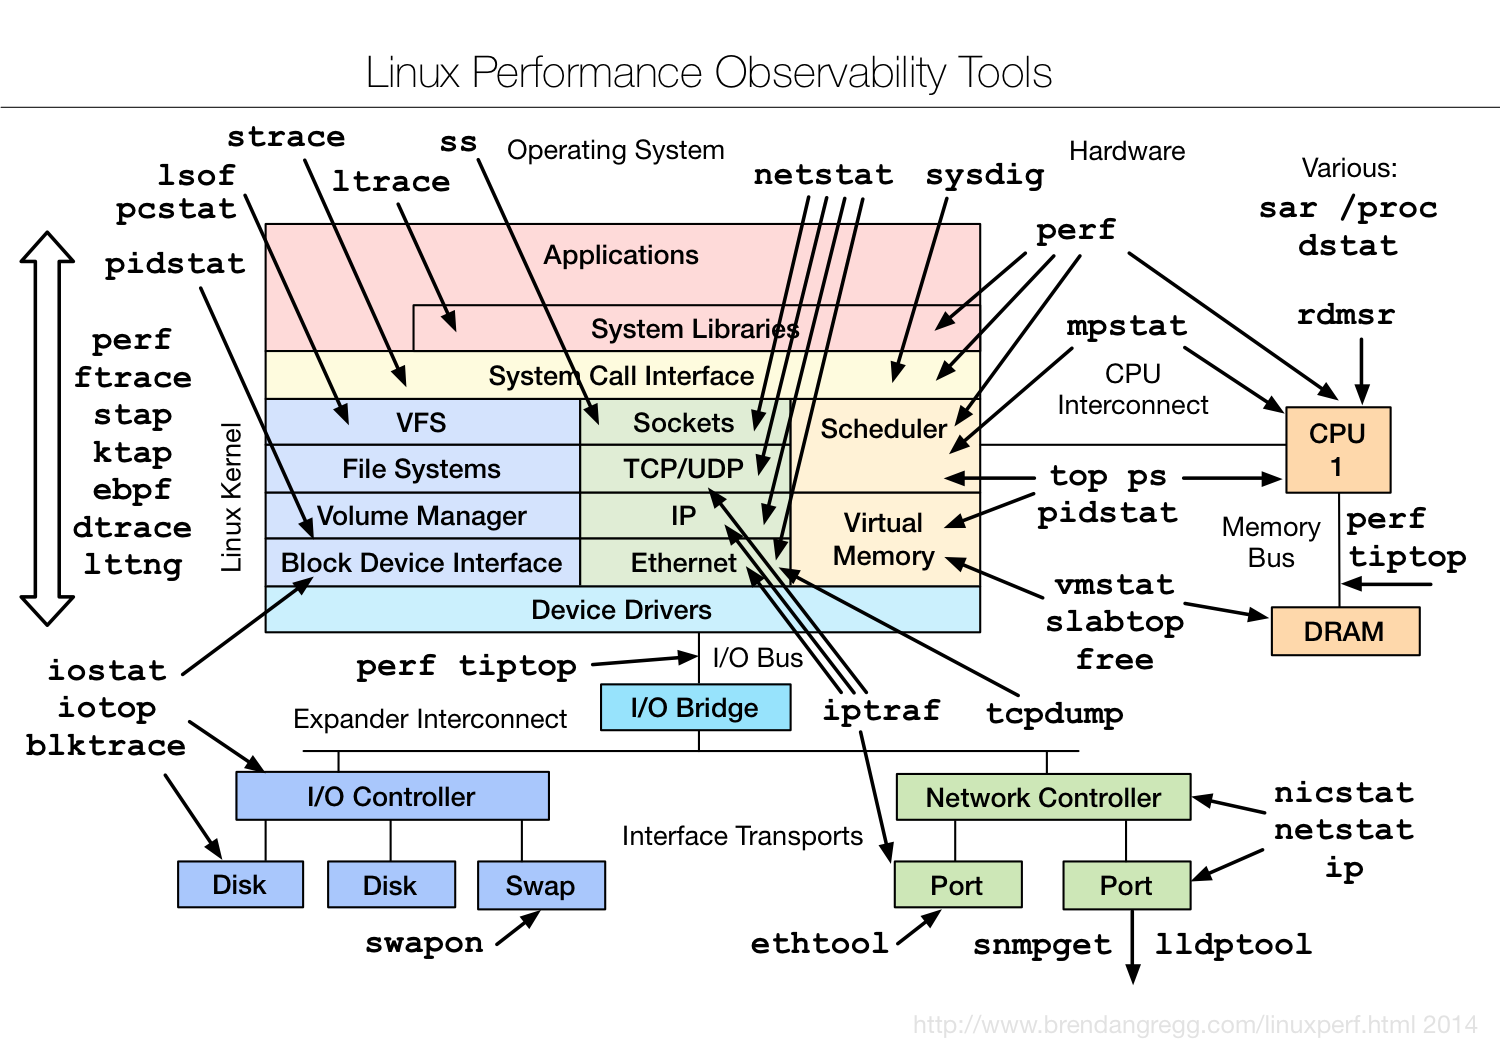
\includegraphics[height=0.75\textheight]{../../slides/profile/linux_observability_tools.png}\footnote{\url{http://www.brendangregg.com/linuxperf.html}}

\end{frame}


\begin{frame}
  \frametitle{Методы профилирования}
  \begin{itemize}
    \item Добавление в код дополнительных инструкций (gprof)
      \begin{enumerate}
        \item[Достоинства] Не требуется поддержка ядра
        \item[Недостатки] Рекомпиляция, замедление кода
      \end{enumerate}
    \item Статистическое исследование (oprofile,perf)
      \begin{enumerate}
        \item[Достоинства] Малое вмешательство в процесс, скорость
        \item[Недостатки] Требуется модуль ядра, точность
      \end{enumerate}
    \item Эмуляция процессора для перехвата вызовов (valgrind)
       \begin{enumerate}
         \item[Достоинства] Не требуется рекомпиляция и модули ядра
         \item[Недостатки] Скорость
        \end{enumerate}
    \item Перехват системных и библиотечных вызовов (strace,ltrace)
       \begin{enumerate}
          \item[Достоинства] Нет рекомпиляции, любое ядро
          \item[Недостатки] Недостаточная информативность
       \end{enumerate}
  \end{itemize}
\end{frame}

}
\section{Gprof}
\mode<all>{\begin{frame}[fragile]
 \frametitle{Gprof}
 \begin{itemize}
   \item Компилировать с опцией \texttt{-pg}
\begin{lstlisting}[language=sh]
 gcc -g -pg -o program program.c
\end{lstlisting}
   \item Создается файл gmon.out
   \item Просмотр статистики (плоский профиль, flat profile) 
\begin{lstlisting}[language=sh]
gprof program -p
\end{lstlisting}
    \item Просмотр графа вызовов со статистикой
\begin{lstlisting}[language=sh]
gprof program -q
\end{lstlisting}
    \item Аннотация исходного кода
\begin{lstlisting}[language=sh]
gprof program -A
\end{lstlisting}
 \end{itemize}
\end{frame}

\begin{frame}
  \frametitle{Упражнение}
  \begin{enumerate}
    \item Написать программу, которая в цикле вызывает функции a и b, b также вызывается внутри a
    \item Скомпилировать с флагом \textt{-pg}
    \item Просмотреть информацию профайлером
  \end{enumerate}
\end{frame}

}
\section{Профилирование в valgrind}
\mode<all>{\begin{frame}[fragile]
 \frametitle{Valgrind callgrind}
 \begin{itemize}
  \item Инструмент для профилирования \verb+ --tool=callgrind+
  \item Просмотр результатов
    \begin{itemize}
      \item \texttt{kcachegrind}
      \item \texttt{callgrind\_annotate}
    \end{itemize}
 \end{itemize}
% \begin{center}
%  Упражнение
% \end{center}
% \begin{enumerate}
%  \item Скомпилировать ту же самую программу с ключами \verb+-g+
%  \item Запустить под valgrind
%  \item Изучить callgraph и относительное время в функциях
% \end{enumerate}
\end{frame}


\begin{frame}[fragile]
    \frametitle{Упражнение}
    \begin{enumerate}
        \item Создаем рандомный файл с необходимым размером: {\tt dd if=/dev/urandom of=input bs=5M count=1}
        \item {\tt time gzip input -c >/dev/null}
        \item Запускаем с помощью valgrind: \\
	    {\tt time valgrind --tool=callgrind gzip input} \\
	    Ждем.
        \item Сравниваем результаты по времени.
        \item Смотрим появившийся файл callgrind.out.\$PID
        \item Запускаем: kcachegrind callgrind.out.\$PID
	\item Смотрим получившийся callgraph и относительное время в функциях.
        \item Запускаем: callgrind\_annotate callgrind.out.\$PID
    \end{enumerate}
\end{frame}
}
\section[oprofile]{Статистическое профилирование в oprofile}
\mode<all>{\begin{frame}
 \frametitle{Статистический сбор образцов: общие соображения}
 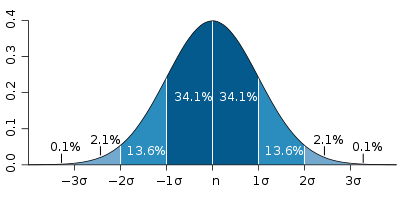
\includegraphics[width=0.7\textwidth]{../../slides/profile/Standard_deviation_diagram.png}
 \begin{itemize}
   \item Распределение Пуассона, в пределе больших $n$ переходящее в нормальное распределение
   \item Ширина распределения $\sim \sqrt{n}$
 \end{itemize}
\end{frame}

\begin{frame}
\frametitle{Инструменты для сбора статистики}
\begin{itemize}
\item oprofile
\item perf
\end{itemize}
\end{frame}

\begin{frame}
  \frametitle{Устройство perf}
  \begin{itemize}
    \item Внутриядерные компоненты (обеспечивают syscall)
    \item Утилита perf (user space)
  \end{itemize}
\end{frame}

\begin{frame}
 \frametitle{Компоненты oprofile}
  \begin{itemize}
    \item Модуль ядра oprofile
    \item Системный демон \texttt{oprofiled}
    \item Программы управления \texttt{opcontrol,opannotate,}
  \end{itemize}
\end{frame}

\begin{frame}[fragile]
 \frametitle{Проверка поддержки perf в ядре}
 \begin{itemize}
   \item \verb+ grep PERF <configure>+
   \item Где найти \texttt{.configure}
     \begin{itemize}
      \item \texttt{.configure} В исходниках ядра
      \item \verb+/boot/configure-`uname -r`+
      \item \verb+/proc/config.gz+
     \end{itemize}
  \end{itemize}
\end{frame} 

\begin{frame}[fragile]
 \frametitle{Запуск oprofile: Проверка поддержки в ядре}
 \begin{itemize}
   \item \verb+ grep OPROFILE <configure>+
 \end{itemize}
\end{frame} 

\begin{frame}[fragile]
 \frametitle{Основные команды perf}
 \begin{itemize}
   \item \verb+ perf record <program> <args>+
   \item \verb+ perf report+
   \item \verb+ perf annotate -d <program file>+
   \item \verb+ perf top+
   \item \verb+ perf stat+
 \end{itemize}
\end{frame}

\begin{frame}[fragile]
 \frametitle{Запуск oprofile: Работа}
 \begin{itemize}
  \item \verb+ opcontrol --no-vmlinux+ 
  \item \verb+ opcontrol --init+
  \item \verb+ opcontrol --start; ./my_program ; opcontrol --dump;  opcontrol --stop+
  \item \verb+ opannotate --source ./my_program +
 \end{itemize}
\end{frame}

\begin{frame}[fragile]
 \frametitle{Упражнение}
 \begin{enumerate}
  \item Проверить, что в конфигурации ядра есть поддержка perf
  \item Установить perf \verb+apt-get update; apt-get install perf +
  \item Скомпилировать программу с \texttt{-g}
  \item Запустить под perf
  \item Посмотреть статистику вызовов
  \item Запустить еще раз
  \item Посмотреть статистику еще раз, сравнить
 \end{enumerate}
\end{frame}
}
\section{Анализ тестового покрытия}
\mode<all>{\begin{frame}{Введение}
  \begin{itemize}
    \item Введение
    \item Возможности
    \item Обзор архитектуры
    \item Примеры, примеры, примеры 
    \item Нюансы использования
    \item NFSTrace: Пример
  \end{itemize}
\end{frame}

\begin{frame}{Введение}
  \begin{center}
    \Large Зачем все это?
  \end{center}
\end{frame}

\begin{frame}{Перед тем как наченм}
  \begin{block}{Sir Charles Dilke, 1892 г.}
    Существует три вида лжи: ложь, наглая ложь и статистика.
  \end{block}
\end{frame}

\begin{frame}{Возможности}
  \begin{itemize}
    \item Как часто выполняется каждая строчка кода\footnote{покрытие по функциям, веткам исполнения}
    \item Какие именно строки кода были выполнены
    \item Как много времени программа проводит в каждой секции кода
  \end{itemize}
\end{frame}

\begin{frame}{Ключи компиляции gcc}
  \begin{itemize}
    \item O0 (компиляция без оптимизации)
    \item Ключ -ftest-coverage (после компиляции: gcno )
    \item Ключ -fprofile-arcs (после запуска:  gcda)
    \item -{}-coverage (2 ключа объединены)
  \end{itemize}
\end{frame}

\begin{frame}{Архитектура: Базовый блок}
    \begin{block}{Базовый блок}
        Последовательность инструкций, имеющая одну точку входа и одну точку выхода.
    \end{block}
\end{frame}

\begin{frame}{Архитектура: gcno файл}
  \begin{itemize}
    \item Файл создается после компиляции
    \item Граф базовых блоков
    \item Маппинг базовых блоков на строки кода
  \end{itemize}
\end{frame}

\begin{frame}{Архитектура: gcda файл}
  \begin{itemize}
      \item Создается после выполнения программы
      \item Создается для каждого объектного файла\footnote{скомпилированного с опцией -fprofile-arcs}
      \item Содержит статистику исполнения программы
  \end{itemize}
\end{frame}


\begin{frame}{Архитектура: gcda файл}
  \begin{center}
    \large Накапливает статистику для каждого запуска!\footnote{Более подробно: gcov-io.h}
  \end{center}
\end{frame}

\begin{frame}{Архитектура: gcov файл}
  \begin{itemize}
      \item gcov [ключи] [SOURCE|OBJ]
      \item На выходе *.gcov файл
      \item Подробная информация об исполнении
  \end{itemize}
\end{frame}

\begin{frame}{gcov: ключи}
  \begin{itemize}
      \item Функциональные для анализа: a, b, c, f, u
      \item Вспомогательные для деплоймента: p, r, f, o, s
      \item Остальные: m, i, d
  \end{itemize}
\end{frame}

\begin{frame}{Нюансы использования}
  \begin{itemize}
      \item Сложный код (несколько инструкций на одной строке)
      \item Макросы
      \item Виртуальные функции/деструкторы (Пример 4)  
  \end{itemize}
\end{frame}

\begin{frame}{Пример 1 (часть 1)}
  \begin{enumerate}
      \item Зайти в директории hello
      \item vi makefile (ключи компиляции)
      \item vi hello.c 
      \item make (появится hello.gcno)
      \item ./hello 1 (появится hello.gcda)
      \item gcov hello.c (появится hello.c.gcov)
      \item vi hello.c.gcov
  \end{enumerate}
\end{frame}

\begin{frame}{Пример 1 (часть 2)}
  \begin{enumerate}
      \item ./hello 1
      \item gcov hello.c (посмотреть что изменилось)
      \item ./hello 2
      \item gcov hello.c
      \item vi hello.c.gcov 
      \item ./hello 3
      \item gcov hello.c (100\%)
  \end{enumerate}
\end{frame}

\begin{frame}{Пример 2 (ветвление)}
  \begin{enumerate}
      \item Удалить 2 if из hello.c
      \item make clean
      \item make
      \item ./hello 1
      \item gcov -b hello.c (branch taken / branch executed)\footnote{Обратить внимание на количесвто branch-ей}
      \item ./hello 2 
      \item gcov -b hello.c (branch taken / branch executed)
  \end{enumerate}
\end{frame}

\begin{frame}{Пример 3 (статистика по функцииям)}
  \begin{enumerate}
      \item Перейти в каталог core
      \item Изучить core.c core.h main.c
      \item make
      \item ./core
      \item gcov -f core (статистика по фукнциям)
      \item Добавить вызов Calc2 в main.c
      \item Посмотреть как изменится статистика
  \end{enumerate}
\end{frame}

\begin{frame}{Пример 4 (виртуальный деструктор)}
  \begin{enumerate}
      \item Перейт в каталог ctor
      \item Изучить makefile (параметр gcov)
      \item Запустить make gcov
      \item Обратить внимание на строку "Taken at least once 50\% of 2"
      \item Объяснить полученый результат\footnote{Дополнительная информация: \url{http://stackoverflow.com/questions/7199360/what-is-the-branch-in-the-destructor-reported-by-gcov}}
  \end{enumerate}
\end{frame}

\begin{frame}{Пример 5 (когда 100\% != все строки кода)}
  \begin{enumerate}
      \item Перейт в каталог hello100 
      \item make 
      \item ./hello100 1 
      \item gcov hello100 
      \item Обратить внимание на строку "Lines executed:100.00\%"
  \end{enumerate}
\end{frame}


\begin{frame}{Пример: NFSTrace}
  \begin{center}
    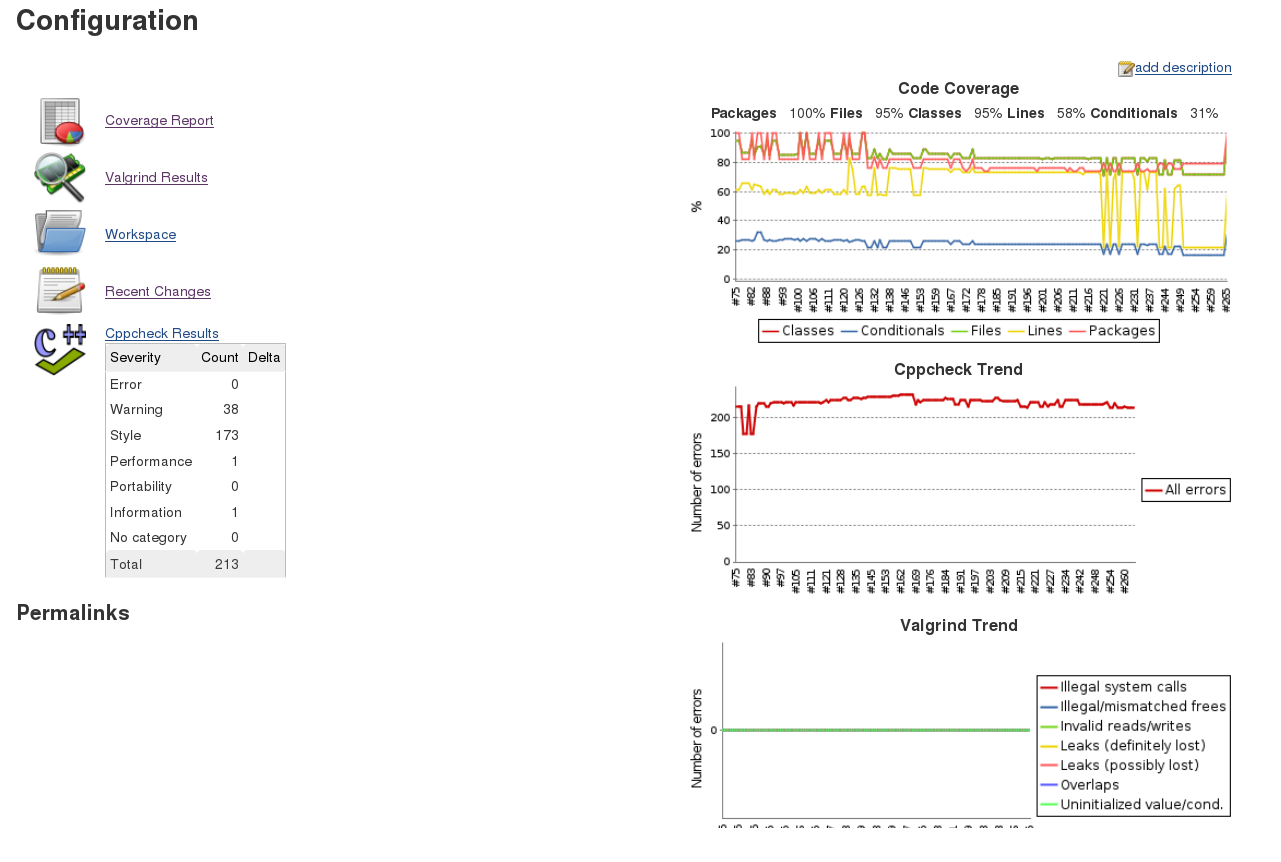
\includegraphics[height=0.9\textheight]{../../slides/profile/nfs-trace-coverage.png}
  \end{center}
\end{frame}

\begin{frame}{Пример: NFSTrace}
  \begin{center}
    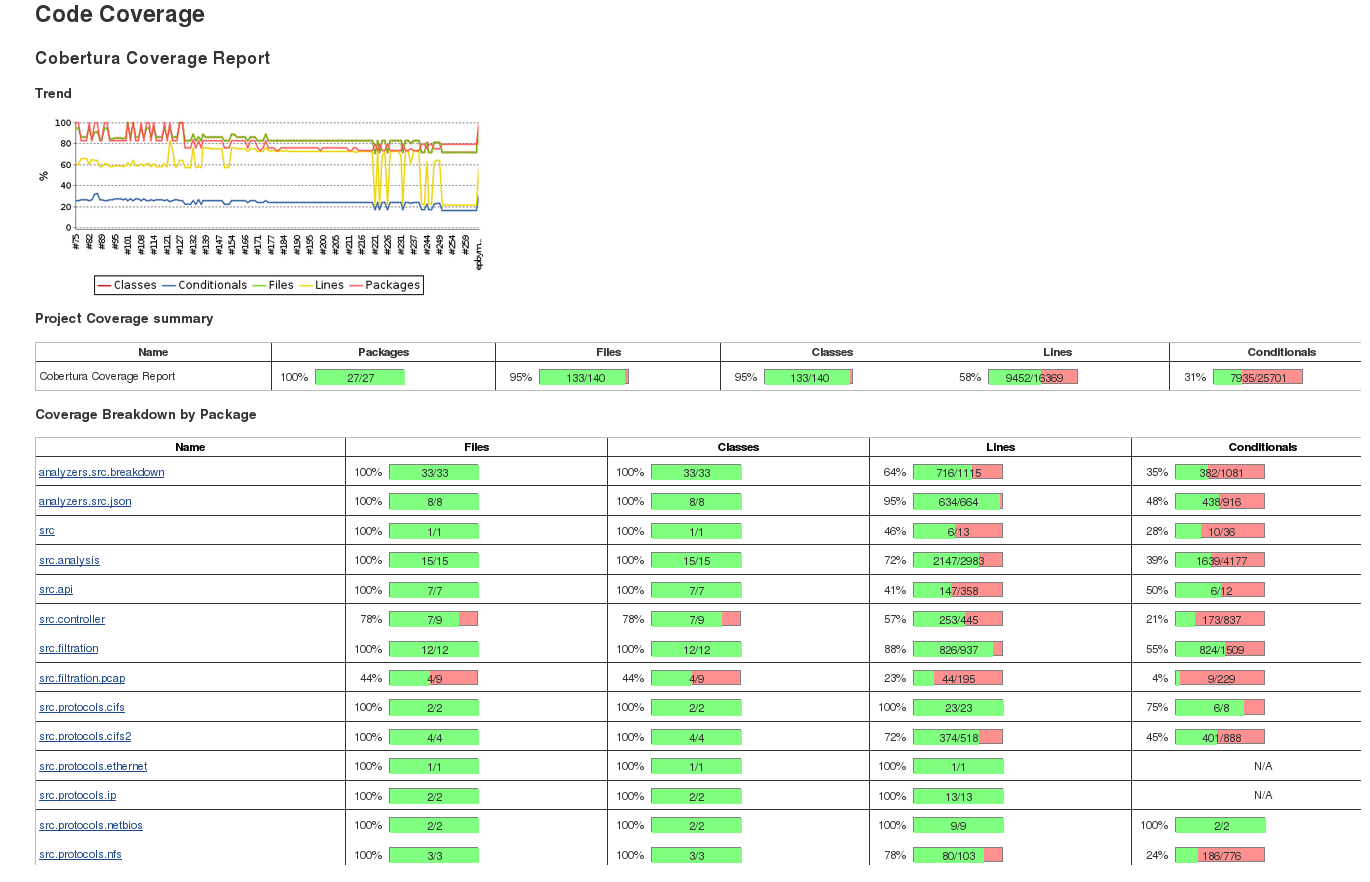
\includegraphics[height=0.9\textheight]{../../slides/profile/nfs-trace-coverage-html.png}
  \end{center}
\end{frame}

}

\chapter{Пакетирование}
\section{Введение}
\mode<all>{\begin{frame}
	\frametitle{И еще раз про "DLL hell"}
	
	\begin{block}{Устанавливаем программу}
	А что же с библиотеками?
	\end{block}

	\pause

	\begin{columns}
		\column{0.5\textwidth}
		\begin{block}{"В системе все есть!"}
		\begin{itemize}
			\item Oh, really???
			\item И нужной версии?
			\item А API и ABI точно не менялись?
			\item А если библиотек несколько версий?
			\item А если нужны дополнительные программы?
		\end{itemize}
		\end{block}
		\pause
		\column{0.5\textwidth}
		\begin{block}{"Всё своё, ношу с собой!"}
		\begin{itemize}
			\item А как насчет объема?
			\item Использование памяти.
			\item А что насчет лицензий?
			\item И все-таки порядок загрузки...
			\item Не спасает от проблем с 3rd-party ПО.
		\end{itemize}
		\end{block}
	\end{columns}
\end{frame}

\begin{frame}
	\frametitle{Хаос}

	\begin{center}
		"Даешь каждой платформе и языку собственную систему управления пакетами!"
	\end{center}

	\begin{block}{Увы, мы не в идеальном мире}
		\begin{itemize}
			\item Дистрибутивы: rpm\{4,5\}, deb, portage, pacman... и куча модификаций...
			\item Дополнительный софт: {\tt ./configure; make; make install}
			\item Java: {\tt ivy, ant, maven, gradle}
			\item Ruby: gem
			\item Perl: CPAN
			\item Python: pip + PyPi
		\end{itemize}
	\end{block}

\end{frame}

\begin{frame}
	\frametitle{Разработка и использование в реальной системе}
	
	\begin{block}{Build-time vs Run-time}

		\begin{enumerate}
			\item Не все, что нужно во время компиляции, должно быть установлено в конечной системе.
			\item Не все, что нужно для работы программы, необходимо устанавливать на сборочной системе.
		\end{enumerate}
	\end{block}
%TODO перенести после описания структуры каталогов
	\begin{block}{Чистое сборочное окружение}
		\begin{itemize}
			\item Воспроизводимость сборки 
			\item Контроль зависимостей
			\item Контроль автоматически "подхваченных" зависимостей
		\end{itemize}
	\end{block}
\end{frame}

}
\section{RPM}
\mode<all>{\begin{frame}
%damn tilde, best that i found
\def~{$\sim$}
	\frametitle{Подготовка окружения для сборки}	
			\begin{itemize}
				\item {\tt rpmdevtools} -- разные полезные помощники
				\item {\tt rpmdev-setuptree} -- создает структуру каталогов
				\item {\tt ~/.rpmmacros} -- информация о пакетировщике, локальные
			\end{itemize}			
				\begin{table}
					\begin{tabular}{l | l | l }
					Каталог & Макрос & Описание\\
					\hline
					~/RPM/SPECS/ & \%\_specdir & Сборочные .spec файлы\\
					~/RPM/SOURCES/ & \%\_sourcedir & Исходные архивы и патчи\\
					\hline
					~/RPM/BUILD/ & \%\_builddir	& Сборка\\		
					~/RPM/BUILDROOT/ & \%\_buildrootdir & Установка\\
					\hline
					~/RPM/RPMS/ & \%\_rpmdir & Собранные .rpm\\
					~/RPM/SRPMS/ & \%\_srcrpmdir & ``Собранный'' .srpm \\
					\end{tabular}
				\end{table}			
\end{frame}

\begin{frame}
\def~{$\sim$}
\frametitle{Пример 0: Hello, World!}

	\begin{block}{Упражнение: hello.spec}
		\begin{itemize}
			\item Скопировать файл описания сборки {\tt hello.spec} в {\tt ~/RPM/SPECS/}
			\item Скопировать файл c исходным кодом в {\tt ~/RPM/SOURCES/}
			\item Собрать пакет с помощью {\tt rpmbuild -ba ~/RPM/SPECS/hello.spec}
			\item Посмотреть получившуюся файловую структуру {\tt find ~/RPM/}
		\end{itemize}
	\end{block}

\end{frame}

\begin{frame}
	\frametitle{Шаги сборки}
	
			\begin{table}
				\begin{tabular}{l | l | l | l }
				Шаг & Чтение & Запись & Описание \\
				\hline 
				\%prep & \%\_sourcedir & \%\_builddir & Подготовка\\
				\%build & \%\_builddir & \%\_builddir & Сборка (configure, make)\\
				\%install & \%\_builddir & \%\_buildrootdir & Установка (make install)\\
				\%check &	\%\_builddir & \%\_builddir & Проверка (make test)\\
				\hline 
				bin & \%\_buildrootdir	&\%\_rpmdir & Упаковка RPM\\
				src & \%\_sourcedir & \%\_srcrpmdir & Упаковка SRPM\\
				\end{tabular}
			\end{table}
\end{frame}

\begin{frame}
	\frametitle{Структура spec-файла}
	\begin{itemize}
		\item Тэги -- {\tt Tag: value}
		\begin{itemize}
		\item Все из открытого шаблона .spec файла
		\item Отсутствующие в шаблоне
			\begin{itemize}
			\item {\tt Patch0: } имя файла с патчем
			\item {\tt BuildArch/ExcludeArch/ExclusiveArch: } архитектура (noarch)
			\item {\tt BuildRoot: } BUILDROOT каталог устарело
			\end{itemize}
		\item Зависимости
			\begin{itemize}
			\item {\tt BuildRequires:}
			\item {\tt Requires:}
			\item {\tt Provides:}
			\item {\tt Conflicts:}
			\item {\tt Obsoletes:}
			\item {\tt AutoReqProv: (0|1)}
			\end{itemize}
		\end{itemize}
	\end{itemize}
\end{frame}

\begin{frame}
	\frametitle{Структура spec-файла}

	\begin{itemize}
		\item Секции --  {\tt \%prep, \%build, \%install, \%check, \%files, \%changelog} 
		\item Макросы -- {\tt \%define FOO bar} 
		\item Скриптлеты, выполняемые в различных условиях\\
			{\tt (pre-,post-)install, uninstall, trigger}
		\item Подпакеты -- {\tt \%package}
		\item Условности -- {\tt \%ifarch ARCH\_NAME, \%if TRUE\_OR\_FALSE}
	\end{itemize}
	\begin{block}{Hint:}
		 {\tt rpm -\-showrc }
	\end{block}
\end{frame}

\begin{frame}
	\frametitle{Пример 1: Hello, World!}

	\begin{block}{Упражнение: hello.spec}
		\begin{itemize}
			\item Собрать пакет с помощью {\tt rpmbuild -ba hello.spec}
			\item Посмотреть список зависимостей {\tt rpm -qRp hello*.rpm}
			\item Установить полученный пакет
			\begin{itemize}
				\item {\tt apt-cache dotty template > template.dot}
				\item {\tt dot -Tpng template.dot -o template.png}
			\end{itemize}
			\item Удалить исходники и spec-файл
			\item Пересобрать пакет из SRPM {\tt rpmbuild -{}-rebuild *.src.rpm}
		\end{itemize}
	\end{block}

	\pause

	\begin{block}{Упражнение: расширяем функционал}
		Добавить компиляцию, установку и пакетирование для CPP-примера.
	\end{block}

\end{frame}


\begin{frame}
	\frametitle{Разработка и использование в реальной системе}
	
	\begin{block}{Build-time vs Run-time}

		\begin{enumerate}
			\item Не все, что нужно во время компиляции, должно быть установлено в конечной системе.
			\item Не все, что нужно для работы программы, необходимо устанавливать на сборочной системе.
		\end{enumerate}
	\end{block}
	\begin{block}{Чистое сборочное окружение}
		\begin{itemize}
			\item Воспроизводимость сборки 
			\item Контроль зависимостей
			\item Контроль автоматически "подхваченных" зависимостей
		\end{itemize}
	\end{block}
\end{frame}

\begin{frame}
	\frametitle{Версии}

	\Large{Чтение правил дистрибутива строго обязательно!}
	
	Hint: {\tt rpmdev-vercmp (rpmdevtools)}
	\begin{block}{ Версия -- составная}
		{\tt \%name-\%epoch:\%version-\%release}
		\begin{itemize}
			\item {\tt Name: == \%name}
			\item {\tt Epoch: == \%epoch}
			\item {\tt Version: == \%version}
			\item {\tt Release: == \%release}
			\begin{itemize}
				\item Release:
				\item \%\{?dist\} tag
				\item rebuild number -- автоматически (при использовании нормальных билд-систем)
			\end{itemize}
		\end{itemize}
	\end{block}

\end{frame}


\begin{frame}
	\frametitle{Пример 2}

	\begin{block}{Подпакеты, скрипты, зависимости и обновление}
		На примере {\tt template.spec}:

		\begin{itemize}
			\item Собрать пакет с помощью {\tt rpmbuild -ba template.spec}
			\item Посмотреть список зависимостей {\tt rpm -qRp template*.rpm}
			\item Установить полученные пакеты
			\item Изменить версию, пересобрать и обновить в системе
			\item Построить дерево зависимостей:
			\item Удалить полученные пакеты
		\end{itemize}
	\end{block}
\end{frame}

\begin{frame}
	\frametitle{Задача на дом: Пакетируем linking}

	\begin{block}{Задача:}
		Создать и установить пакеты для примера с созданием библиотек
		и их использования из предыдущих лекций.
	\end{block}

	Hint: libtestA, libtestB, libtestA-devel, libtestB-devel, mainpkg

\end{frame}

}

\chapter{Системы контроля версий}
\section{Введение}
\mode<all>{\begin{frame}
 \frametitle{История систем контроля версий}
 \begin{enumerate}
  \item[1972] SCCS
  \item[1982] RCS (Revision control system)
  \item[1990] CVS Concurrent version system
  \item[2000] Subversion(SVN)
  \item[2000] BitKeeper(proprietary)
  \item[2003] Monotone, darcs
  \item[2005] Git, Bazaar, Mercurial
 \end{enumerate}
\end{frame}

\begin{frame}
 \frametitle{Распределенные и централизованные системы контроля версий}
 \begin{columns}
  \column{0.5\textwidth}
   \begin{center}
     Централизованные (CVS,SVN)
   \end{center}
   \begin{itemize}
    \item Достоинства
     \begin{itemize}
       \item Линейная история изменений
       \item Не надо хранить весь репозиторий
       \item Лучшая поддержка бинарных файлов
     \end{itemize}
    \item Недостатки
     \begin{itemize}
       \item Single point of failure
       \item Трудно работать без доступа к сети
       \item Общая тормознутость
     \end{itemize}
   \end{itemize}
  \column{0.5\textwidth}
   \begin{center}
     Распределенные
   \end{center}
   \begin{itemize}
    \item Достоинства
     \begin{itemize}
       \item Не задушишь, не убьешь
       \item Часто быстрее
       \item Более гибкая работа в команде
       \item Не требуют сети для основной работы
     \end{itemize}
    \item Недостатки
     \begin{itemize}
       \item Большой репозиторий на локальной машине
       \item Невозможность замка на бинарном файле
       \item Зоопарк версий
     \end{itemize}
   \end{itemize}
 \end{columns}
\end{frame}
}
\section[SVN]{Subversion}
\mode<all>{\begin{frame}
 \frametitle{Базовые команды для работы с svn клиентом}
  \begin{itemize}
   \item svn help
   \item svn checkout 
   \item svn import
   \item svn update
   \item svn commit
   \item svn status
   \item svn copy
   \item svn switch
  \end{itemize}
\end{frame}

\begin{frame}
 \frametitle{Типичная последовательность действий при работе с svn}
 \begin{itemize}
  \item svn import my_project svn://myhost.com/my_project/trunk
  \item $\dots$
  \item svn checkout svn://myhost.com/my_project/trunk myproject
  \item Редактируем файлы в директории myproject
  \item svn status -- смотрим изменения
  \item svn diff
  \item svn update 
  \item Разрешаем конфликты
  \item svn commit --user me --password mypass -m "Some changes"
  \item svn update
 \end{itemize}
\end{frame}

\begin{frame}
 \frametitle{Типичная структура svn репозитория}
 \begin{itemize}
  \item project1
    \begin{itemize}
      \item trunk
        \begin{itemize}
          \item file1.txt
          \item $\dots$
        \end{itemize}
      \item tags
      \item branches
         \begin{itemize}
            \item branch1
            \item branch2
         \end{itemize}
     \end{itemize}
  \item project2

 \end{itemize}
\end{frame}

\begin{frame}
 \frametitle{Как создавать svn репозиторий}
 \begin{itemize}
   \item svnadmin
     \begin{itemize}
       \item svnadmin help
       \item svnadmin create <путь к директории>
     \end{itemize}
    \item svnserve
      \begin{itemize}
        \item svnserve -d -r <путь к репозиторию>
        \item Файлы настройки: conf/passwd, conf/svnserve.conf
      \end{itemize}
\end{frame}

\begin{frame}
 \frametitle{Упражнение}
  \begin{itemize}
    \item Поднять svn репозиторий на localhost
    \item Внести в него файлы из проекта rpm
    \item Сделать svn checkout всего проекта в отдельную директорию
    \item Отредактировать несколько файлов в созданной директории
    \item Закоммитить изменения в центральный репозиторий
    \item Создать ветку от исходной ревизии
  \end{itemize}
\end{frame}
}
\section{Git}
\mode<all>{\begin{frame}
 \frametitle{Основные команды git}
\end{frame}

\begin{frame}
 \frametitle{Типичные действия в git}
 \begin{itemize}
  \item git init
  \item git add file1 file2 file3
  \item git commit -m "First revision"
  \item $\dots$
  \item git branch new-branch
  \item git checkout new-branch
  \item Редактируем файлы в новой ветке
  \item git commit -a -m "Какое-то изменение"
  \item Повторить по вкусу
  \item git checkout master 
  \item git merge new-branch master
  \item git rebase 
  \item git push origin master
 \end{itemize}
\end{frame}

\begin{frame}
 \frametitle{Внутреннее устройство git}
\end{frame}

\begin{frame}
 \frametitle{Упражнение}
\end{frame}
}

\part*{Информация}

Актуальная версия исходников:\\
\url{https://github.com/epam-llpd/linux_courses}

Актуальная версия скомпилированных документов:\\
\url{https://yadi.sk/d/S4HA4z6lqdMNQ}

\bigskip

\begin{enumerate}
		\item Денис Пынькин
		\item Юрий Адамов
		\item Павел Корнелюк
		\item Викентий Лапа
		\item Евгений Рыбак
		\item {\it Здесь может быть Ваша фамилия}
\end{enumerate}

\end{document}
